%%%%%%%%%%%%%%%%%%%%%%%%%%%%%%%%%%%%%%%%%%%%%%%%%%%%%%%%%%%%%%%%%
% Contents: Main Input File of the LaTeX2e Introduction
% $Id: lshort-base.tex 447 2010-12-14 14:32:00Z oetiker $
%%%%%%%%%%%%%%%%%%%%%%%%%%%%%%%%%%%%%%%%%%%%%%%%%%%%%%%%%%%%%%%%%
% lshort.tex - The not so short introduction to LaTeX   
%                                                      by Tobias Oetiker
%                                                     oetiker@ee.ethz.ch
%
%                           based on LKURTZ.TEX Uni Graz & TU Wien, 1987
%-----------------------------------------------------------------------
%
% To compile lshort, you need TeX 3.x, LaTeX and makeindex
%
% The sources files of the Intro are:
%      lshort.tex (this file),
%      titel.tex, contrib.tex, biblio.tex
%      things.tex, typeset.tex, math.tex, lssym.tex, spec.tex,
%      lshort.sty, fancyheadings.sty
%
% Further the  verbatim.sty and the layout.sty 
% from the LaTeX Tools distribution is
% required.
%
%
% To print the AMS symbols you need the AMS fonts and the packages
% amsfonts, eufrak and eucal from (AMS LaTeX 1.2)
%
% ---------------------------------------------------------------------

%%%%%%%%%%%%%%%%%%%%%%%%%%%%%%%%%%%%%%%%%%%%%%%%%%%%%%%%%%%%%%%%%
% Contents: Who contributed to this Document
% $Id: contrib.tex 457 2011-04-06 09:50:23Z oetiker $
%%%%%%%%%%%%%%%%%%%%%%%%%%%%%%%%%%%%%%%%%%%%%%%%%%%%%%%%%%%%%%%%%
\begin{small} 
  \noindent Copyright \copyright 1995-2011 Tobias Oetiker and Contributors.  All rights reserved.
 
  This document is free; you can redistribute it and/or modify it
  under the terms of the GNU General Public License as published by
  the Free Software Foundation; either version 2 of the License, or
  (at your option) any later version.
  
  This document is distributed in the hope that it will be useful, but
  \emph{without any warranty}; without even the implied warranty of
  \emph{merchantability} or \emph{fittness for a particular purpose}\@.  See the GNU
  General Public License for more details.
  
  You should have received a copy of the GNU General Public License
  along with this document; if not, write to the Free Software
  Foundation, Inc., 675 Mass Ave, Cambridge, MA 02139, USA.

\end{small}

\chapter{Thank you!}
\noindent Much of the material used in this introduction comes from an
Austrian introduction to \LaTeX\ 2.09 written in German by:
\begin{verse}
\contrib{Hubert Partl}{partl@mail.boku.ac.at}%
{Zentraler Informatikdienst der Universit\"at f\"ur Bodenkultur Wien}
\contrib{Irene Hyna}{Irene.Hyna@bmwf.ac.at}%
   {Bundesministerium f\"ur Wissenschaft und Forschung Wien}
\contrib{Elisabeth Schlegl}{no email}%
   {in Graz}
\end{verse}

If you are interested in the German document, you can find a version
updated for \LaTeXe{} by J\"org Knappen at
\CTAN|info/lshort/german|

\newpage \noindent The
following individuals helped with corrections, suggestions and
material to improve this paper. They put in a big effort to help me
get this document into its present shape. I would like to
sincerely thank all of them. Naturally, all the mistakes you'll find
in this book are mine. If you ever find a word that is spelled
correctly, it must have been one of the people below dropping me a
line.

{ \flushleft\small
Eric~Abrahamsen,        %eric@ericabrahamsen.net
Rosemary~Bailey,        %r.a.bailey@qmw.ac.uk 0.2
Marc~Bevand,            % <bevand_m@epita.fr>
Friedemann~Brauer,      %fbrauer@is.dal.ca 3.4
Barbara~Beeton,         %bnb@ams.org
Salvatore~Bonaccorso,   % bonaccos@ee.ethz.ch
Jan~Busa,               % <busaj@ccsun.tuke.sk>
Markus~Br\"uhwiler,     % <m.br@switzerland.org>
Pietro~Braione,         % <braione@elet.polimi.it>
David~Carlisle,         %GONE carlisle@cs.man.ac.uk 1.0
Jos\'e~Carlos~Santos,   % <jcsantos@fc.up.pt>
Neil~Carter,            % N.Carter@Swansea.ac.uk
Mike~Chapman,           %chapman@eeh.ee.ethz.ch 3.16
Pierre~Chardaire,       % <pc@sys.uea.ac.uk
Christopher~Chin,       %chris.chin@rmit.edu.au 3.1
Carl~Cerecke,           %cdc@cosc.canterbury.ac.nz>
Chris~McCormack,        %GONE chrismc@eecs.umich.edu 0.1
Diego~Clavadetscher,    % DC@clavatax.ch
Wim~van~Dam,            %GONE wimvdam@cs.kun.nl 2.2
Benjamin~Deschwanden    % vdeschwb@student.ethz.ch
Jan~Dittberner,         %jan@jan-dittberner.de 3.15
Michael~John~Downes,    %<mjd@ams.org> 14 Oct 1999
Matthias~Dreier,        %dreier@ostium.ch
David~Dureisseix,       %dureisse@lmt.ens-cachan.fr 1.1
Eilinger~August,        % <eaugust@student.ethz.ch>
Elliot,                 %GONE enh-a@minster.york.ac.uk 1.1
Rockrush~Engch,         %niatlantice@gmail.com
Hans~Ehrbar,            %ehrbar@econ.utah.edu
Daniel~Flipo,           %Daniel.Flipo@univ-lille1.fr
David~Frey,             %david@eos.lugs.ch 2.2
Hans~Fugal,             %hans@fugal.net
Robert~Funnell,         %<robert.funnell@mcgill.ca>
Robin~Fairbairns,       %Robin.Fairbairns@cl.cam.ac.uk 0.2 1.0
J\"org~Fischer,        %j.fischer@xpoint.at 3.16
Erik~Frisk,             %frisk@isy.liu.se 3.4
Mic~Milic~Frederickx,   % <mic.milic@web.de>
Frank,                  %frank@freezone.co.uk 11 Feb 2000
Kasper~B.~Graversen,    % <kbg@dkik.dk>
Arlo~Griffiths,         % <A.Griffiths@let.leidenuniv.nl>
Alexandre~Guimond,      %guimond@IRO.UMontreal.CA 0.9
Andy~Goth,              % <unununium@openverse.com>
Cyril~Goutte,           %goutte@ei.dtu.dk 2.1 2.2
Greg~Gamble,            %gregg@maths.uwa.edu.au 2.2
Frank~Fischli,          % <fischlifaenger@gmx.ch>
Robert~Funnell,         % <robert.funnell@mcgill.ca> 5.1
Morten~H�gholm,		% morten.hoegholm@latex-project.org
Neil~Hammond,           %nfh@dmu.ac.uk 0.3
Rasmus~Borup~Hansen,    %GONE rbhfamos@math.ku.dk 0.2 0.9 0.91 0.92 1.9.9
Joseph~Hilferty,        % <hilferty@fil.ub.es>
Bj\"orn Hvittfeldt,     %bjorn@hvittfeldt.com 3.13
Martien~Hulsen,         %M.A.Hulsen@WbMt.TUDelft.NL 1.0 1.1
Werner~Icking,          %<Werner.Icking@gmd.de> 3.1
Jakob,                  %diness@get2net.dk
Eric~Jacoboni,          %GONE jacoboni@enseeiht.fr 0.1 0.9
Alan~Jeffrey,           %alanje@cogs.sussex.ac.uk 0.2
Byron~Jones,            %bj@dmu.ac.uk 1.1
David~Jones,            %GONE djones@CA.McMaster.dcss.insight 1.1
Nils~Kanning,           % <nils@kanning.de>
Tobias~Krewer,          %tobias.krewer@googlemail.com
Johannes-Maria~Kaltenbach, %<kaltenbach@zeiss.de> 3.01
Andrzej~Kawalec,        %GONE akawalec@prz.rzeszow.pl 1.9.9
Sander~de~Kievit,       %Skievit@ucu.uu.nl
Alain~Kessi,            %ALAIN_KESSI@HOTMAIL.COM 2.2
Christian~Kern,         %ck@unixen.hrz.uni-oldenburg.de 2.1
Tobias~Klauser,		%tklauser@access.unizh.ch 4.17
J\"org~Knappen,         %knappen@vkpmzd.kph.uni-mainz.de 0.1
Kjetil~Kjernsmo,        %<kjetil.kjernsmo@astro.uio.no> 3.2
Michael~Koundouros,     % <mkoundouros@hotmail.com>
Matt~Kraai,             % <Matt.Kraai@amo.abbott.com>
Maik~Lehradt,           %greek@uni-paderborn.de 0.1
R\'emi~Letot,           % <r_letot@yahoo.com>
Flori~Lambrechts,       % <f.lambrechts@softhome.net>
Mike~Lee,               % rmrstar@gmail.com
Axel~Liljencrantz,	% <Axel.Liljencrantz@byv.kth.se>
Johan~Lundberg,         %p99jlu@physto.se
Alexander~Mai,          %Alexander.Mai@physik.tu-darmstadt.de 3.8
Hendrik~Maryns,         %hendrik.maryns@ugent.be
Martin~Maechler,        %<maechler@stat.math.ethz.ch> 2.2
Aleksandar~S~Milosevic, % <aleksandar.milosevic@yale.edu>
Henrik~Mitsch,          % <Henrik.Mitsch@gmx.at>
Claus~Malten,           %GONE <ASI138%BITNET.DJUKFA11@BITNET.CEARN> 1.1
Kevin~Van~Maren,        % <vanmaren@fast.cs.utah.edu>  24 Nov 1999
Stefan~M.~Moser,        % stefan.moser@ieee.org 
Richard~Nagy,           % r.nagy@nameshield.net
Philipp~Nagele,         % Philipp.Nagele@t-systems.com
Lenimar~Nunes~de~Andrade, % <lenimar@mat.ufpb.br> Fri, 12 Nov 1999
I.~J.~Vera~Mar\'un,    % I.J.Veramarun@ewi.utwente.nl
Manuel~Oetiker,         % manuel@oetiker.ch
Urs~Oswald,             % osurs@bluewin.ch
Marcelo~Pasin,          %<pasin@di.fc.ul.pt>
Lan~Thuy~Pham,          %<lan.thuy.pham@gmail.com>
Martin~Pfister,		% m@rtinpfister.ch
Breno~Pietracci,        % <bpietracci@gmail.com>
Demerson~Andre~Polli,   % polli@linux.ime.usp.br
Nikos~Pothitos,		% <n.pothitos@di.uoa.gr>
Maksym~Polyakov         % <polyama@myrealbox.com>
Hubert~Partl,           %partl@mail.boku.ac.at 0.2 1.1
John~Refling,           %refling@sierra.lbl.gov 0.1 0.9
Mike~Ressler,           %ressler@cougar.jpl.nasa.gov 0.1 0.2 0.9 1.0 1.9.9
Brian~Ripley,           %ripley@stats.ox.ac.uk 2.1
Young~U.~Ryu,           %ryoung@utdallas.edu 2.1
Bernd~Rosenlecher,      %9rosenle@informatik.uni-hamburg.de 10 Feb 2000
Kurt~Rosenfeld,		%kurt@isis.poly.edu
Chris~Rowley,           %C.A.Rowley@open.ac.uk 0.91
Axel~Kielhorn,          % a.kielhorn@web.de
Risto~Saarelma,         %risto.saarelma@cs.helsinki.fi
Jordi~Serra~i~Solanich, %solanich@gmail.com
Hanspeter~Schmid,       %schmid@isi.ee.ethz.ch
Craig~Schlenter,        %cschle@lucy.ee.und.ac.za 0.1 0.2 0.9
Gilles~Schintgen,       %gschintgen@internet.lu
Baron~Schwartz,         % <bps7j@cs.virginia.edu>      
Christopher~Sawtell,    %<csawtell@xtra.co.nz> 1 Sep 1999
Miles~Spielberg,        %zeibach@hotmail.com
Matthieu~Stigler,       % table row height
Geoffrey~Swindale,      % <geofftswin@ntlworld.com>
Laszlo~Szathmary,       % <szathml@delfin.klte.hu>
Andr{\'a}s~Salamon,        % Andras.Salamon@comlab.ox.ac.uk
Boris~Tobotras,         % <tobotras@jet.msk.su>
Josef~Tkadlec,          %tkadlec@math.feld.cvut.cz 2.0 2.2
Scott~Veirs,            %scottv@ocean.washington.edu
Didier~Verna,           %verna@inf.enst.fr 2.2
Matthew~Widmann,        % <mtwdmn@gmail.com>
Fabian~Wernli,          %wernli@iap.fr 3.2
Carl-Gustav~Werner,     % <Carl-Gustav.Werner@math.lu.se> 11 Oct 1999,3.16
David~Woodhouse,        % <dwmw2@infradead.org> 3.16
Chris~York,             % <c.s.york@Cummins.com>  21 Nov 1999
Fritz~Zaucker,          %zaucker@ee.ethz.ch 3.0
Rick~Zaccone,           %zaccone@bucknell.edu 2.2
and Mikhail~Zotov.      %zotov@eas.npi.msu.su 3.1

}

\vspace*{\stretch{1}}



\pagebreak
\endinput
%

% Local Variables:
% TeX-master: "lshort2e"
% mode: latex
% mode: flyspell
% End:

%%%%%%%%%%%%%%%%%%%%%%%%%%%%%%%%%%%%%%%%%%%%%%%%%%%%%%%%%%%%%%%%%
% Contents: Who contributed to this Document
% $Id: overview.tex 456 2011-04-06 09:10:27Z oetiker $
%%%%%%%%%%%%%%%%%%%%%%%%%%%%%%%%%%%%%%%%%%%%%%%%%%%%%%%%%%%%%%%%%

% Because this introduction is the reader's first impression, I have
% edited very heavily to try to clarify and economize the language.
% I hope you do not mind! I always try to ask "is this word needed?"
% in my own writing but I don't want to impose my style on you... 
% but here I think it may be more important than the rest of the book.
% --baron

\chapter{Preface}

\LaTeX{} \cite{manual} is a typesetting system that is very 
suitable for producing scientific and mathematical documents of high
typographical quality. It is also suitable for producing all
sorts of other documents, from simple letters to complete books.
\LaTeX{} uses \TeX{} \cite{texbook} as its formatting engine.

This short introduction describes \LaTeXe{} and should be sufficient
for most applications of \LaTeX. Refer to~\cite{manual,companion} for
a complete description of the \LaTeX{} system.

\bigskip
\noindent This introduction is split into 6 chapters:
\begin{description}
\item[Chapter 1] tells you about the basic structure of \LaTeXe{}
  documents. You will also learn a bit about the history of \LaTeX{}.
  After reading this chapter, you should have a rough understanding how
  \LaTeX{} works.
\item[Chapter 2] goes into the details of typesetting your
  documents. It explains most of the essential \LaTeX{} commands and
  environments. After reading this chapter, you will be able to write
  your first documents. 
\item[Chapter 3] explains how to typeset formulae with \LaTeX. Many
  examples demonstrate how to use one of \LaTeX{}'s
  main strengths. At the end of the chapter are tables listing
  all mathematical symbols available in \LaTeX{}.
\item[Chapter 4] explains indexes,  bibliography generation and
  inclusion of EPS graphics. It introduces creation of PDF documents with pdf\LaTeX{}
  and presents some handy extension packages.
\item[Chapter 5] shows how to use \LaTeX{} for creating graphics. Instead
  of drawing a picture with some graphics program, saving it to a file and
  then including it into \LaTeX{}, you describe the picture and have \LaTeX{}
  draw it for you.
\item[Chapter 6] contains some potentially dangerous information about
  how to alter the
  standard document layout produced by \LaTeX{}. It will tell you how  to
  change things such that the beautiful output of \LaTeX{}
  turns ugly or stunning, depending on your abilities.
\end{description}
\bigskip
\noindent It is important to read the chapters in order---the book is
not that big, after all. Be sure to carefully read the examples,
because a lot of the information is in the
examples placed throughout the book.

\bigskip
\noindent \LaTeX{} is available for most computers, from the PC and Mac to large
UNIX and VMS systems. On many university computer clusters you will
find that a \LaTeX{} installation is available, ready to use.
Information on how to access
the local \LaTeX{} installation should be provided in the \guide. If
you have problems getting started, ask the person who gave you this
booklet. The scope of this document is \emph{not} to tell you how to
install and set up a \LaTeX{} system, but to teach you how to write
your documents so that they can be processed by~\LaTeX{}.

\bigskip
\noindent If you need to get hold of any \LaTeX{} related material, 
have a look at one of the Comprehensive \TeX{} Archive Network
(CTAN) sites. The homepage is at
\url{http://www.ctan.org}.

You will find other references to CTAN throughout the book, especially
pointers to software and documents you might want to download. Instead
of writing down complete urls, I just wrote \texttt{CTAN:} followed by
whatever location within the CTAN tree you should go to.

If you want to run \LaTeX{} on your own computer, take a look at what
is available from \CTAN|systems|.

\vspace{\stretch{1}}
\noindent If you have ideas for something to be
added, removed or altered in this document, please let me know. I am
especially interested in feedback from \LaTeX{} novices about which
bits of this intro are easy to understand and which could be explained
better.

\bigskip
\begin{verse}
\contrib{Tobias Oetiker}{tobi@oetiker.ch}%
\noindent{OETIKER+PARTNER AG\\Aarweg 15\\4600 Olten\\Switzerland}
\end{verse}
\vspace{\stretch{1}}
\noindent The current version of this document is available on\\
\CTAN|info/lshort|

\endinput



%

% Local Variables:
% TeX-master: "lshort2e"
% mode: latex
% mode: flyspell
% End:

\tableofcontents
\listoffigures
\listoftables
\enlargethispage{\baselineskip}
\mainmatter
%%%%%%%%%%%%%%%%%%%%%%%%%%%%%%%%%%%%%%%%%%%%%%%%%%%%%%%%%%%%%%%%%
% Contents: Things you need to know
% $Id: things.tex 456 2011-04-06 09:10:27Z oetiker $
%%%%%%%%%%%%%%%%%%%%%%%%%%%%%%%%%%%%%%%%%%%%%%%%%%%%%%%%%%%%%%%%%
 
\chapter{Things You Need to Know}
\begin{intro}
The first part of this chapter presents a short 
overview of the philosophy and history of \LaTeXe. The second part
focuses on the basic structures of a \LaTeX{} document. 
After reading this chapter, you should have a rough knowledge
of how \LaTeX{} works, which you will need to understand the rest
of this book.  
\end{intro}

\section{The Name of the Game}
\subsection{\TeX}
 
\TeX{} is a computer program created by \index{Knuth, Donald E.}Donald
E. Knuth \cite{texbook}. It is aimed at typesetting text and
mathematical formulae. Knuth started writing the \TeX{} typesetting
engine in 1977 to explore the potential of the digital printing
equipment that was beginning to infiltrate the publishing industry at
that time, especially in the hope that he could reverse the trend of
deteriorating typographical quality that he saw affecting his own
books and articles. \TeX{} as we use it today was released in 1982,
with some slight enhancements added in 1989 to better support 8-bit
characters and multiple languages. \TeX{} is renowned for being
extremely stable, for running on many different kinds of computers,
and for being virtually bug free. The version number of \TeX{} is
converging to $\pi$ and is now at $3.141592653$.
                                                                       
\TeX{} is pronounced ``Tech,'' with a ``ch'' as in the German word
``Ach''\footnote{In german there are actually two pronounciations for ``ch''
and one might assume that the soft ``ch'' sound from ``Pech'' would be a
more appropriate. Asked about this, Knuth wrote in the German Wikipedia:
\emph{I do not get angry when people pronounce \TeX{} in their favorite way
\ldots{} and in Germany many use a soft ch because the X follows the vowel
e, not the harder ch that follows the vowel a. In Russia, `tex' is a very
common word, pronounced `tyekh'. But I believe the most proper pronunciation
is heard in Greece, where you have the harsher ch of ach and Loch.}}
or in the Scottish ``Loch.'' The ``ch'' originates from the Greek
alphabet where X is the letter ``ch'' or ``chi''. \TeX{} is also the first syllable
of the Greek word {\greektext teknolog'ia} (technology). In an ASCII environment, \TeX{}
becomes \texttt{TeX}.

\subsection{\LaTeX}
 
\LaTeX{} enables authors to typeset and print their work at the highest
typographical quality, using a predefined, professional layout. \LaTeX{} was
originally written by \index{Lamport, Leslie}Leslie Lamport~\cite{manual}.
It uses the \TeX{} formatter as its typesetting engine. These days \LaTeX{}
is maintained by \index{Mittelbach, Frank}Frank Mittelbach.

%In 1994 the \LaTeX{} package was updated by the \index{LaTeX3@\LaTeX
%  3}\LaTeX 3 team, led by \index{Mittelbach, Frank}Frank Mittelbach,
%to include some long-requested improvements, and to re\-unify all the
%patched versions which had cropped up since the release of
%\index{LaTeX 2.09@\LaTeX{} 2.09}\LaTeX{} 2.09 some years earlier. To
%distinguish the new version from the old, it is called \index{LaTeX
%2e@\LaTeXe}\LaTeXe. This documentation deals with \LaTeXe. These days you
%might be hard pressed to find the venerable \LaTeX{} 2.09 installed
%anywhere.

\LaTeX{} is pronounced ``Lay-tech'' or ``Lah-tech.'' If you refer to
\LaTeX{} in an ASCII environment, you type \texttt{LaTeX}.
\LaTeXe{} is pronounced ``Lay-tech two e'' and typed \texttt{LaTeX2e}.

%Figure~\ref{components} above % on page \pageref{components}
%shows how \TeX{} and \LaTeXe{} work together. This figure is taken from
%\texttt{wots.tex} by Kees van der Laan.

%\begin{figure}[btp]
%\begin{lined}{0.8\textwidth}
%\begin{center}
%\input{kees.fig}
%\end{center}
%\end{lined}
%\caption{Components of a \TeX{} System.} \label{components}
%\end{figure}

\section{Basics}
 
\subsection{Author, Book Designer, and Typesetter}

To publish something, authors give their typed manuscript to a
publishing company. One of their book designers then
decides the layout of the document (column width, fonts, space before
and after headings,~\ldots). The book designer writes his instructions
into the manuscript and then gives it to a typesetter, who typesets the
book according to these instructions.

A human book designer tries to find out what the author had in mind
while writing the manuscript. He decides on chapter headings,
citations, examples, formulae, etc.\ based on his professional
knowledge and from the contents of the manuscript.

In a \LaTeX{} environment, \LaTeX{} takes the role of the book
designer and uses \TeX{} as its typesetter. But \LaTeX{} is ``only'' a
program and therefore needs more guidance. The author has to provide
additional information to describe the logical structure of his
work. This information is written into the text as ``\LaTeX{}
commands.''

This is quite different from the \wi{WYSIWYG}\footnote{What you see is
  what you get.} approach that most modern word processors, such as
\emph{MS Word} or \emph{LibreOffice}, take. With these
applications, authors specify the document layout interactively while
typing text into the computer. They can see on the
screen how the final work will look when it is printed.

When using \LaTeX{} it is not normally possible to see the final output
while typing the text, but the final output can be previewed on the
screen after processing the file with \LaTeX. Then corrections can be
made before actually sending the document to the printer.

\subsection{Layout Design}

Typographical design is a craft. Unskilled authors often commit
serious formatting errors by assuming that book design is mostly a
question of aesthetics---``If a document looks good artistically,
it is well designed.'' But as a document has to be read and not hung
up in a picture gallery, the readability and understandability is 
much more important than the beautiful look of it.
Examples: 
\begin{itemize}
\item The font size and the numbering of headings have to be chosen to make
  the structure of chapters and sections clear to the reader.
\item The line length has to be short enough not to strain
  the eyes of the reader, while long enough to fill the page
  beautifully.
\end{itemize}

With \wi{WYSIWYG} systems, authors often generate aesthetically
pleasing documents with very little or inconsistent structure.
\LaTeX{} prevents such formatting errors by forcing the author to
declare the \emph{logical} structure of his document. \LaTeX{} then
chooses the most suitable layout.

\subsection{Advantages and Disadvantages}

When people from the \wi{WYSIWYG} world meet people who use \LaTeX{},
they often discuss ``the \wi{advantages of \LaTeX{}} over a normal
word processor'' or the opposite.  The best thing to do when such
a discussion starts is to keep a low profile, since such discussions
often get out of hand. But sometimes there is no escaping \ldots

\medskip\noindent So here is some ammunition. The main advantages
of \LaTeX{} over normal word processors are the following:

\begin{itemize}

\item Professionally crafted layouts are available, which make a
  document really look as if ``printed.''
\item The typesetting of mathematical formulae is supported in a
  convenient way.
\item Users only need to learn a few easy-to-understand commands
  that specify the logical structure of a document. They almost never
  need to tinker with the actual layout of the document.
\item Even complex structures such as footnotes, references, table of
  contents, and bibliographies can be generated easily.
\item Free add-on packages exist for many typographical tasks not directly supported by basic
  \LaTeX. For example, packages are
  available to include \PSi{} graphics or to typeset
  bibliographies conforming to exact standards. Many of these add-on
  packages are described in \companion.
\item \LaTeX{} encourages authors to write well-structured texts,
  because this is how \LaTeX{} works---by specifying structure.
\item \TeX, the formatting engine of \LaTeXe, is highly portable and free.
  Therefore the system runs on almost any hardware platform
  available. 

%
% Add examples ...
%
\end{itemize}

\medskip

\noindent\LaTeX{} also has some disadvantages, and I guess it's a bit
difficult for me to find any sensible ones, though I am sure other people
can tell you hundreds \texttt{;-)}

\begin{itemize}
\item \LaTeX{} does not work well for people who have sold their
  souls \ldots
\item Although some parameters can be adjusted within a predefined
  document layout, the design of a whole new layout is difficult and
  takes a lot of time.\footnote{Rumour says that this is one of the
    key elements that will be addressed in the upcoming \LaTeX 3
    system.}\index{LaTeX3@\LaTeX 3}
\item It is very hard to write unstructured and disorganized documents.
\item Your hamster might, despite some encouraging first steps, never be
able to fully grasp the concept of Logical Markup.
\end{itemize}

\section{\LaTeX{} Input Files}

The input for \LaTeX{} is a plain text file. On Unix/Linux text files are
pretty common. On windows, one would use Notepad to create a text file. It
contains the text of the document, as well as the commands that tell
\LaTeX{} how to typeset the text. If you are working with a LaTeX IDE, it will contain a program for creating
\LaTeX{} input files in text format.

\subsection{Spaces}

``Whitespace'' characters, such as blank or tab, are
treated uniformly as ``\wi{space}'' by \LaTeX{}. \emph{Several
  consecutive} \wi{whitespace} characters are treated as \emph{one}
``space.''  Whitespace at the start of a line is generally ignored, and
a single line break is treated as ``whitespace.''
\index{whitespace!at the start of a line}

An empty line between two lines of text defines the end of a
paragraph. \emph{Several} empty lines are treated the same as
\emph{one} empty line. The text below is an example. On the left hand
side is the text from the input file, and on the right hand side is the
formatted output.

\begin{example}
It does not matter whether you
enter one or several     spaces
after a word.

An empty line starts a new 
paragraph.
\end{example}
 
\subsection{Special Characters}

The following symbols are \wi{reserved characters} that either have a
special meaning under \LaTeX{} or are not available in all the fonts.
If you enter them directly in your text, they will normally not print,
but rather coerce \LaTeX{} to do things you did not intend. 
\begin{code}
\verb.#  $  %  ^  &  _  {  }  ~  \ . %$
\end{code}

As you will see, these characters can be used in your documents all
the same by using a prefix backslash:

\begin{example}
\# \$ \% \^{} \& \_ \{ \} \~{}
\textbackslash
\end{example}

The other symbols and many more can be printed with special commands
in mathematical formulae or as accents. The backslash character
\textbackslash{} can \emph{not} be entered by adding another backslash
in front of it (\verb|\\|); this sequence is used for
line breaking. Use the \ci{textbackslash} command instead.

\subsection{\LaTeX{} Commands}

\LaTeX{} \wi{commands} are case sensitive, and take one of the following
two formats:

\begin{itemize}
\item They start with a \wi{backslash} \verb|\| and then have a name
 consisting of letters only. Command names are terminated by a
 space, a number or any other `non-letter.'
\item They consist of a backslash and exactly one non-letter.
\item Many commands exist in a `starred variant' where a star is appended
to the command name.
\end{itemize}

%
% \\* doesn't comply !
%

%
% Can \3 be a valid command ? (jacoboni)
%
\label{whitespace}

\LaTeX{} ignores whitespace after commands. If you want to get a
\index{whitespace!after commands}space after a command, you have to
put either an empty parameter \verb|{}| and a blank or a special spacing command after the
command name. The empty parameter \verb|{}| stops \LaTeX{} from eating up all the white space after
the command name. 

\begin{example}
I read that Knuth divides the 
people working with \TeX{} into 
\TeX{}nicians and \TeX perts.\\
Today is \today.
\end{example}

Some commands require a \wi{parameter}, which has to be given between
\wi{curly braces} \verb|{ }| after the command name. Some commands take
\wi{optional parameters}, which are inserted after the command name in
\wi{square brackets}~\verb|[ ]|.
\begin{code}
\verb|\|\textit{command}\verb|[|\textit{optinal parameter}\verb|]{|\textit{parameter}\verb|}|
\end{code}
The next examples use some \LaTeX{}
commands. Don't worry about them; they will be explained later.

\begin{example}
You can \textsl{lean} on me!
\end{example}
\begin{example}
Please, start a new line
right here!\newline
Thank you!
\end{example}

\subsection{Comments}
\index{comments}

When \LaTeX{} encounters a \verb|%| character while processing an input file,
it ignores the rest of the present line, the line break, and all
whitespace at the beginning of the next line.

This can be used to write notes into the input file, which will not show up
in the printed version.

\begin{example}
This is an % stupid
% Better: instructive <----
example: Supercal%
              ifragilist%
    icexpialidocious
\end{example}

The \texttt{\%} character can also be used to split long input lines where no
whitespace or line breaks are allowed.

For longer comments you could use the \ei{comment} environment
provided by the \pai{verbatim} package. Add the
line \verb|\usepackage{verbatim}| to the preamble of your document as
explained below to use this command.

\begin{example}
This is another
\begin{comment}
rather stupid,
but helpful
\end{comment}
example for embedding
comments in your document.
\end{example}

Note that this won't work inside complex environments, like math for example.

\section{Input File Structure}

When \LaTeXe{} processes an input file, it expects it to follow a
certain \wi{structure}. Thus every input file must start with the
command
\begin{code}
\verb|\documentclass{...}|
\end{code}
This specifies what sort of document you intend to write. After that,
add commands to influence the style of the whole
document, or load \wi{package}s that add new
features to the \LaTeX{} system. To load such a package you use the
command
\begin{code}
\verb|\usepackage{...}|
\end{code}

When all the setup work is done,\footnote{The area between \texttt{\bs
    documentclass} and \texttt{\bs
    begin$\mathtt{\{}$document$\mathtt{\}}$} is called the
  \emph{\wi{preamble}}.} you start the body of the text with the
command

\begin{code}
\verb|\begin{document}|
\end{code}

Now you enter the text mixed with some useful \LaTeX{} commands.  At
the end of the document you add the
\begin{code}
\verb|\end{document}|
\end{code}
command, which tells \LaTeX{} to call it a day. Anything that
follows this command will be ignored by \LaTeX.

Figure~\ref{mini} shows the contents of a minimal \LaTeXe{} file. A
slightly more complicated \wi{input file} is given in
Figure~\ref{document}.

\begin{figure}[!bp]
\begin{lined}{6cm}
\begin{verbatim}
\documentclass{article}
\begin{document}
Small is beautiful.
\end{document}
\end{verbatim}
\end{lined}
\caption{A Minimal \LaTeX{} File.} \label{mini}
\end{figure}
 
\begin{figure}[!bp]
\begin{lined}{10cm}
\begin{verbatim}
\documentclass[a4paper,11pt]{article}
% define the title
\author{H.~Partl}
\title{Minimalism}
\begin{document}
% generates the title
\maketitle 
% insert the table of contents
\tableofcontents
\section{Some Interesting Words}
Well, and here begins my lovely article.
\section{Good Bye World}
\ldots{} and here it ends.
\end{document}
\end{verbatim}
\end{lined}
\caption[Example of a Realistic Journal Article.]{Example of a Realistic
Journal Article. Note that all the commands you see in this example will be
explained later in the introduction.} \label{document}

\end{figure}

\section{A Typical Command Line Session}

I bet you must be dying to try out the neat small \LaTeX{} input file
shown on page \pageref{mini}. Here is some help:
\LaTeX{} itself comes without a GUI or
fancy buttons to press. It is just a program that crunches away at your
input file. Some \LaTeX{} installations feature a graphical front-end where
there is a \LaTeX{} button to start compiling your input file. On other systems
there might be some typing involved, so here is how to coax \LaTeX{} into
compiling your input file on a text based system. Please note: this
description assumes that a working \LaTeX{} installation already sits on
your computer.\footnote{This is the case with most well groomed Unix
Systems, and \ldots{} Real Men use Unix, so \ldots{} \texttt{;-)}}

\begin{enumerate}
\item 
  
  Edit/Create your \LaTeX{} input file. This file must be plain ASCII
  text.  On Unix all the editors will create just that. On Windows you
  might want to make sure that you save the file in ASCII or
  \emph{Plain Text} format.  When picking a name for your file, make
  sure it bears the extension \eei{.tex}.

\item 

Open a shell or cmd window, cd to the directory where your input file is located and run \LaTeX{} on your input file. If successful you will end up with a
\texttt{.dvi} file. It may be necessary to run \LaTeX{} several times to get
the table of contents and all internal references right. When your input
file has a bug \LaTeX{} will tell you about it and stop processing your
input file. Type \texttt{ctrl-D} to get back to the command line.
\begin{lscommand}
\verb+latex foo.tex+
\end{lscommand}

\item 
Now you may view the DVI file. There are several ways to do that. Look at the file on screen with
\begin{lscommand}
\verb+xdvi foo.dvi &+
\end{lscommand}
This only works on Unix with X11. If you are on Windows you might want to try \texttt{yap} (yet another previewer).

Convert the dvi file to \PSi{} for printing or viewing with \wi{GhostScript}.
\begin{lscommand}
\verb+dvips -Pcmz foo.dvi -o foo.ps+
\end{lscommand}

If you are lucky your \LaTeX{} system even comes with the \texttt{dvipdf} tool, which allows
you to convert your \texttt{.dvi} files straight into pdf.
\begin{lscommand}
\verb+dvipdf foo.dvi+
\end{lscommand}

\end{enumerate}

 
\section{The Layout of the Document}
 
\subsection {Document Classes}\label{sec:documentclass}

The first information \LaTeX{} needs to know when processing an
input file is the type of document the author wants to create. This
is specified with the \ci{documentclass} command.
\begin{lscommand}
\ci{documentclass}\verb|[|\emph{options}\verb|]{|\emph{class}\verb|}|
\end{lscommand}
\noindent Here \emph{class} specifies the type of document to be created.
Table~\ref{documentclasses} lists the document classes explained in
this introduction. The \LaTeXe{} distribution provides additional
classes for other documents, including letters and slides.  The
\emph{\wi{option}s} parameter customises the behaviour of the document
class. The options have to be separated by commas. The most common options for the standard document
classes are listed in
Table~\ref{options}.


\begin{table}[!bp]
\caption{Document Classes.} \label{documentclasses}
\begin{lined}{\textwidth}
\begin{description}
 
\item [\normalfont\texttt{article}] for articles in scientific journals, presentations,
  short reports, program documentation, invitations, \ldots
  \index{article class}
\item [\normalfont\texttt{proc}] a class for proceedings based on the article class.
  \index{proc class}
\item [\normalfont\texttt{minimal}] is as small as it can get.
It only sets a page size and a base font. It is mainly used for debugging
purposes.
  \index{minimal class}
\item [\normalfont\texttt{report}] for longer reports containing several chapters, small
  books, PhD theses, \ldots \index{report class}
\item [\normalfont\texttt{book}] for real books \index{book class}
\item [\normalfont\texttt{slides}] for slides. The class uses big sans serif
  letters. You might want to consider using the Beamer class instead.
        \index{slides class}
\end{description}
\end{lined}
\end{table}

\begin{table}[!bp]
\caption{Document Class Options.} \label{options}
\begin{lined}{\textwidth}
\begin{flushleft}
\begin{description}
\item[\normalfont\texttt{10pt}, \texttt{11pt}, \texttt{12pt}] \quad Sets the size
  of the main font in the document. If no option is specified,
  \texttt{10pt} is assumed.  \index{document font size}\index{base
    font size}
\item[\normalfont\texttt{a4paper}, \texttt{letterpaper}, \ldots] \quad Defines
  the paper size. The default size is \texttt{letterpaper}. Besides
  that, \texttt{a5paper}, \texttt{b5paper}, \texttt{executivepaper},
  and \texttt{legalpaper} can be specified.  \index{legal paper}
  \index{paper size}\index{A4 paper}\index{letter paper} \index{A5
    paper}\index{B5 paper}\index{executive paper}

\item[\normalfont\texttt{fleqn}] \quad Typesets displayed formulae left-aligned
  instead of centred.

\item[\normalfont\texttt{leqno}] \quad Places the numbering of formulae on the
  left hand side instead of the right.

\item[\normalfont\texttt{titlepage}, \texttt{notitlepage}] \quad Specifies
  whether a new page should be started after the \wi{document title}
  or not. The \texttt{article} class does not start a new page by
  default, while \texttt{report} and \texttt{book} do.  \index{title}

\item[\normalfont\texttt{onecolumn}, \texttt{twocolumn}] \quad Instructs \LaTeX{} to typeset the
  document in \wi{one column} or \wi{two column}s.

\item[\normalfont\texttt{twoside, oneside}] \quad Specifies whether double or
  single sided output should be generated. The classes
  \texttt{article} and \texttt{report} are \wi{single sided} and the
  \texttt{book} class is \wi{double sided} by default. Note that this
  option concerns the style of the document only. The option
  \texttt{twoside} does \emph{not} tell the printer you use that it
  should actually make a two-sided printout.
\item[\normalfont\texttt{landscape}] \quad Changes the layout of the document to print in landscape mode.
\item[\normalfont\texttt{openright, openany}] \quad Makes chapters begin either
  only on right hand pages or on the next page available. This does
  not work with the \texttt{article} class, as it does not know about
  chapters. The \texttt{report} class by default starts chapters on
  the next page available and the \texttt{book} class starts them on
  right hand pages.

\end{description}
\end{flushleft}
\end{lined}
\end{table}

Example: An input file for a \LaTeX{} document could start with the
line
\begin{code}
\ci{documentclass}\verb|[11pt,twoside,a4paper]{article}|
\end{code}
which instructs \LaTeX{} to typeset the document as an \emph{article}
with a base font size of \emph{eleven points}, and to produce a
layout suitable for \emph{double sided} printing on \emph{A4 paper}.
\pagebreak[2]

\subsection{Packages}
\index{package} While writing your document, you will probably find
that there are some areas where basic \LaTeX{} cannot solve your
problem. If you want to include \wi{graphics}, \wi{coloured text} or
source code from a file into your document, you need to enhance the
capabilities of \LaTeX.  Such enhancements are called packages.
Packages are activated with the
\begin{lscommand}
\ci{usepackage}\verb|[|\emph{options}\verb|]{|\emph{package}\verb|}|
\end{lscommand}
\noindent command, where \emph{package} is the name of the package and
\emph{options} is a list of keywords that trigger special features in
the package. Some packages come with the \LaTeXe{} base distribution
(See Table~\ref{packages}). Others are provided separately. You may
find more information on the packages installed at your site in your
\guide. The prime source for information about \LaTeX{} packages is \companion.
It contains descriptions on hundreds of packages, along with
information of how to write your own extensions to \LaTeXe.

Modern \TeX{} distributions come with a large number of packages
preinstalled. If you are working on a Unix system, use the command
\texttt{texdoc} for accessing package documentation.

\begin{table}[btp]
\caption{Some of the Packages Distributed with \LaTeX.} \label{packages}
\begin{lined}{\textwidth}
\begin{description}
\item[\normalfont\pai{doc}] Allows the documentation of \LaTeX{} programs.\\
 Described in \texttt{doc.dtx}\footnote{This file should be installed
   on your system, and you should be able to get a \texttt{dvi} file
   by typing \texttt{latex doc.dtx} in any directory where you have
   write permission. The same is true for all the
   other files mentioned in this table.}  and in \companion.

\item[\normalfont\pai{exscale}] Provides scaled versions of the
  math extension  font.\\ 
  Described in \texttt{ltexscale.dtx}.

\item[\normalfont\pai{fontenc}] Specifies which \wi{font encoding}
  \LaTeX{} should use.\\
  Described in \texttt{ltoutenc.dtx}.

\item[\normalfont\pai{ifthen}] Provides commands of the form\\ 
  `if\ldots then do\ldots otherwise do\ldots.'\\ Described in
  \texttt{ifthen.dtx} and \companion.

\item[\normalfont\pai{latexsym}] To access the \LaTeX{} symbol
  font, you should use the \texttt{latexsym} package. Described in
  \texttt{latexsym.dtx} and in \companion.
 
\item[\normalfont\pai{makeidx}] Provides commands for producing
  indexes.  Described in section~\ref{sec:indexing} and in \companion.

\item[\normalfont\pai{syntonly}] Processes a document without
  typesetting it.
  
\item[\normalfont\pai{inputenc}] Allows the specification of an
  input encoding such as ASCII, ISO Latin-1, ISO Latin-2, 437/850 IBM
  code pages,  Apple Macintosh, Next, ANSI-Windows or user-defined one.
  Described in \texttt{inputenc.dtx}. 
\end{description}
\end{lined}
\end{table}


\subsection{Page Styles}
 
\LaTeX{} supports three predefined \wi{header}/\wi{footer}
combinations---so-called \wi{page style}s. The \emph{style} parameter
of the \index{page style!plain@\texttt{plain}}\index{plain@\texttt{plain}}
\index{page style!headings@\texttt{headings}}\index{headings@texttt{headings}}
\index{page style!empty@\texttt{empty}}\index{empty@\texttt{empty}}
\begin{lscommand}
\ci{pagestyle}\verb|{|\emph{style}\verb|}|
\end{lscommand}
\noindent command defines which one to use. 
Table~\ref{pagestyle}
lists the predefined page styles.

\begin{table}[!hbp]
\caption{The Predefined Page Styles of \LaTeX.} \label{pagestyle}
\begin{lined}{\textwidth}
\begin{description}

\item[\normalfont\texttt{plain}] prints the page numbers on the bottom
  of the page, in the middle of the footer. This is the default page
  style.

\item[\normalfont\texttt{headings}] prints the current chapter heading
  and the page number in the header on each page, while the footer
  remains empty.  (This is the style used in this document)
\item[\normalfont\texttt{empty}] sets both the header and the footer
  to be empty.

\end{description}
\end{lined}
\end{table}

It is possible to change the page style of the current page
with the command
\begin{lscommand}
\ci{thispagestyle}\verb|{|\emph{style}\verb|}|
\end{lscommand}
A description how to create your own
headers and footers can be found in \companion{} and in section~\ref{sec:fancy} on page~\pageref{sec:fancy}.
%
% Pointer to the Fancy headings Package description !
%

\section{Files You Might Encounter}

When you work with \LaTeX{} you will soon find yourself in a maze of
files with various \wi{extension}s and probably no clue. The following
list explains the various \wi{file types} you might encounter when
working with \TeX{}. Please note that this table does not claim to be
a complete list of extensions, but if you find one missing that you
think is important, please drop me a line.

\begin{description}
  
\item[\eei{.tex}] \LaTeX{} or \TeX{} input file. Can be compiled with
  \texttt{latex}.
\item[\eei{.sty}] \LaTeX{} Macro package. Load this
  into your \LaTeX{} document using the \ci{usepackage} command.
\item[\eei{.dtx}] Documented \TeX{}. This is the main distribution
  format for \LaTeX{} style files. If you process a .dtx file you get
  documented macro code of the \LaTeX{} package contained in the .dtx
  file.
\item[\eei{.ins}] The installer for the files contained in the
  matching .dtx file. If you download a \LaTeX{} package from the net,
  you will normally get a .dtx and a .ins file. Run \LaTeX{} on the
  .ins file to unpack the .dtx file.
\item[\eei{.cls}] Class files define what your document looks
  like. They are selected with the \ci{documentclass} command.
\item[\eei{.fd}] Font description file telling  \LaTeX{} about new fonts.
\end{description}
The following files are generated when you run \LaTeX{} on your input
file:

\begin{description}
\item[\eei{.dvi}] Device Independent File. This is the main result of a \LaTeX{}
  compile run. Look at its content with a DVI previewer
  program or send it to a printer with \texttt{dvips} or a
  similar application.
\item[\eei{.log}] Gives a detailed account of what happened during the
  last compiler run.
\item[\eei{.toc}] Stores all your section headers. It gets read in for the
  next compiler run and is used to produce the table of content.
\item[\eei{.lof}] This is like .toc but for the list of figures.
\item[\eei{.lot}] And again the same for the list of tables.
\item[\eei{.aux}] Another file that transports information from one
  compiler run to the next. Among other things, the .aux file is used
  to store information associated with cross-references.
\item[\eei{.idx}] If your document contains an index. \LaTeX{} stores all
  the words that go into the index in this file. Process this file with
  \texttt{makeindex}. Refer to section \ref{sec:indexing} on
  page \pageref{sec:indexing} for more information on indexing.
\item[\eei{.ind}] The processed .idx file, ready for inclusion into your
  document on the next compile cycle.
\item[\eei{.ilg}] Logfile telling what \texttt{makeindex} did.
\end{description}


% Package Info pointer
%
%



%
% Add Info on page-numbering, ...
% \pagenumbering

\section{Big Projects}
When working on big documents, you might want to split the input file
into several parts. \LaTeX{} has two commands that help you to do
that.

\begin{lscommand}
\ci{include}\verb|{|\emph{filename}\verb|}|
\end{lscommand}
\noindent Use this command in the document body to insert the
contents of another file named \emph{filename.tex}. Note that \LaTeX{}
will start a new page
before processing the material input from \emph{filename.tex}.

The second command can be used in the preamble. It allows you to
instruct \LaTeX{} to only input some of the \verb|\include|d files.
\begin{lscommand}
\ci{includeonly}\verb|{|\emph{filename}\verb|,|\emph{filename}%
\verb|,|\ldots\verb|}|
\end{lscommand}
After this command is executed in the preamble of the document, only
\ci{include} commands for the filenames that are listed in the
argument of the \ci{includeonly} command will be executed. Note that
there must be no spaces between the filenames and the commas.

The \ci{include} command starts typesetting the included text on a new
page. This is helpful when you use \ci{includeonly}, because the
page breaks will not move, even when some include files are omitted.
Sometimes this might not be desirable. In this case, use the
\begin{lscommand}
\ci{input}\verb|{|\emph{filename}\verb|}|
\end{lscommand}
\noindent command. It simply includes the file specified. 
No flashy suits, no strings attached.


To make \LaTeX{} quickly check your document use the \pai{syntonly}
package. This makes \LaTeX{} skim through your document only checking for
proper syntax and usage of the commands, but doesn't produce any (DVI) output.
As \LaTeX{} runs faster in this mode you may save yourself valuable time.
Usage is very simple:

\begin{verbatim}
\usepackage{syntonly}
\syntaxonly
\end{verbatim}
When you want to produce pages, just comment out the second line
(by adding a percent sign).


%

% Local Variables:
% TeX-master: "lshort2e"
% mode: latex
% mode: flyspell
% End:

%%%%%%%%%%%%%%%%%%%%%%%%%%%%%%%%%%%%%%%%%%%%%%%%%%%%%%%%%%%%%%%%%
% Contents: Typesetting Part of LaTeX2e Introduction
% $Id: F-700786B269A0D2C3D9A58B999E1CD428.tex,v 1.1 2008-03-06 19:21:17 carleos Exp $
%%%%%%%%%%%%%%%%%%%%%%%%%%%%%%%%%%%%%%%%%%%%%%%%%%%%%%%%%%%%%%%%%
\chapter{Composici�n de texto}

\begin{intro}
  Tras leer el cap�tulo previo, deber�a conocer lo b�sico para
  entender de qu� est� hecho un documento \LaTeXe{}.  En este cap�tulo
  se explica el resto de la estructura que se necesita saber para
  producir un documento �til.
\end{intro}

\section{La estructura del texto y el idioma}
\secby{Hanspeter Schmid}{hanspi@schmid-werren.ch}
El quid de escribir un texto (salvo cierta literatura moderna) es
comunicar ideas, informaci�n o conocimiento al lector.  El lector
entender� mejor el texto si dichas ideas est�n bien estructuradas, y
ver� y sentir� dicha estructura mucho mejor si la forma tipogr�fica
refleja la estructura l�gica y sem�ntica del contenido.

\LaTeX{} se diferencia de otros sistemas de composici�n en que s�lo
tiene que decirle tal estructura.  La forma tipogr�fica del texto se
deriva seg�n las ``reglas'' dadas en el \filenomo{} de clase del documento
y en los varios \filenomo{}s de estilo usados.

La unidad de texto m�s importante en \LaTeX{} (y en tipograf�a) es el
\wi{p�rrafo}.  Lo llamamos ``unidad de texto'' porque un p�rrafo es la
forma tipogr�fica que deber�a reflejar un pensamiento o una
idea b�sica completos.  As�, si
comienza un nuevo pensamiento, deber�a empezar un nuevo p�rrafo; y si no, deber�an usarse
s�lo saltos de l�nea.  Si duda sobre insertar saltos de p�rrafo, recuerde que
su texto es un veh�culo de ideas y pensamientos.  Si tiene un
salto de p�rrafo, pero el anterior pensamiento contin�a, deber�a
eliminar el salto.  Si aparece una l�nea de pensamiento totalmente
nueva en el mismo p�rrafo, entonces deber�a insertar un salto.

Casi todo el mundo subestima completamente la importancia de saltos de
p�rrafo bien situados.  Mucha gente no sabe siquiera cu�l es el
significado de un salto de p�rrafo o, especialmente en \LaTeX,
introduce saltos de p�rrafo sin saberlo.  Este �ltimo error es
especialmente f�cil de cometer si se usan ecuaciones en el texto.
Mire los siguientes ejemplos, y piense por qu� a veces se usan l�neas
vac�as (saltos de p�rrafo) antes y despu�s de la ecuaci�n, y a veces
no.  (Si no entiende bien todav�a todas las �rdenes para entender
estos ejemplos, lea este cap�tulo y el siguiente y luego lea esta
secci�n otra vez.)

\begin{code}
\begin{verbatim}
% Ejemplo 1
...cuando Einstein present� su f�rmula 
\begin{equation} 
  e = m \cdot c^2 \; , 
\end{equation} 
que es al mismo tiempo la f�rmula f�sica 
m�s famosa y la menos entendida.


% Ejemplo 2
...de lo cual se sigue la ley de corrientes de Kirchhoff:
\begin{equation} 
  \sum_{k=1}^{n} I_k = 0 \; .
\end{equation} 

La ley de tensiones de Kirchhoff puede derivarse...


% Ejemplo 3
...lo que tiene varias ventajas.

\begin{equation} 
  I_D = I_F - I_R
\end{equation} 
es el n�cleo de un modelo de transistor muy eficiente. ...
\end{verbatim}
\end{code} 

La siguiente unidad de texto m�s peque�a es la oraci�n.  En textos
ingleses, hay un espacio mayor tras un punto que termina una
oraci�n que tras uno que termina una abreviatura.  \LaTeX{} supone por omisi�n que un punto termina una oraci�n; si se
equivoca, debe indicarle qu� es lo que desea.  Esto se explicar� m�s
tarde en este cap�tulo.  Afortunadamente, en espa�ol no afecta tanto esta distinci�n.

La estructuraci�n de un texto se extiende incluso a partes de las
oraciones.  La mayor�a de los idiomas tienen reglas de puntuaci�n muy
complicadas, pero en muchos idiomas (incluido el espa�ol) acertar�
casi siempre con las comas si recuerda lo que representan: una pausa
breve en el flujo del lenguaje.  Si no est� seguro de d�nde poner una
coma, lea la oraci�n en alto y t�mese un breve respiro en cada coma.
Si le suena mal en alg�n lugar, borre esa coma; si siente que le urge
respirar (o hacer una breve pausa) en otro lugar, inserte una coma.

Finalmente, los p�rrafos de un texto deber�an estar estructurados
tambi�n a un nivel m�s alto, distribuy�ndose en cap�tulos, secciones,
subsecciones, y as� sucesivamente.  Sin embargo, el efecto tipogr�fico
de escribir p.ej.{} \verb|\section{La| \texttt{estructura del texto y
    el idioma}\verb|}| es tan obvio que es casi evidente c�mo deben
usarse estas estructuras de alto nivel.

\section{Saltos de l�nea y de p�gina}
 
\subsection{Justificaci�n de p�rrafos}

Los libros se suelen componer con l�neas de igual longitud.  \LaTeX{}
inserta los \wi{saltos de l�nea} y los espacios necesarios entre
palabras optimizando el contenido de todo un p�rrafo.  Si es preciso,
tambi�n divide palabras con guiones si no caben bien en una l�nea.
C�mo se componen los p�rrafos depende de la clase del documento.
Normalmente la primera l�nea de un p�rrafo lleva sangr�a, y no hay
espacio adicional entre dos p�rrrafos.  Tiene m�s informaci�n al
respecto en la secci�n~\ref{parsp}.

En casos concretos puede ser necesario ordenar a \LaTeX{} que salte de
l�nea: 
\begin{lscommand}
\ci{\bs} � \ci{newline} 
\end{lscommand}
\noindent comienza una nueva l�nea sin comenzar un nuevo p�rrafo.

\begin{lscommand}
\ci{\bs*}
\end{lscommand}
\noindent adem�s proh�be un salto de p�gina tras el salto forzado de l�nea.

\begin{lscommand}
\ci{newpage}
\end{lscommand}
\noindent comienza una nueva p�gina. 

\begin{lscommand}
\ci{linebreak}\verb|[|\emph{n}\verb|]|,
\ci{nolinebreak}\verb|[|\emph{n}\verb|]|, 
\ci{pagebreak}\verb|[|\emph{n}\verb|]|,
\ci{nopagebreak}\verb|[|\emph{n}\verb|]|
\end{lscommand}
\noindent producen un salto de l�nea, impiden un salto de l�nea, producen un salto
de p�gina, o impiden un salto de p�gina, respectivamene.  Permiten al autor ajustar sus
efectos mediante el argumento opcional \emph{n}, al que puede
asignarse un n�mero entre cero y cuatro.  Poniendo \emph{n} a un valor
menor que 4, deja a \LaTeX{} la opci�n de no hacer caso de su orden si
el resultado tiene mal aspecto.  No confunda estas �rdenes ``-break''
con las �rdenes ``new-''.  Incluso si pone una orden ``-break'',
\LaTeX{} a�n intenta dejar bien el borde derecho de la p�gina y la
longitud total de la p�gina, como se describe en la secci�n siguiente.
Si realmente quiere iniciar una nueva l�nea, use la orden ``newline''.

\LaTeX{} siempre intenta prodicir los mejores saltos de p�gina
posibles.  Si no puede encontrar una manera de dividir las l�neas que
cumpla con sus expectativas, permite que una l�nea se salga por la
derecha del p�rrafo.  \LaTeX{} se queja entonces (``\wi{overfull
hbox}'') mientras procesa el \filenomo{} de entrada.  Esto sucede muy a
menudo cuando \LaTeX{} no puede encontrar un lugar adecuado para
dividir una palabra.\footnote{Aunque \LaTeX{} le avisa cuando ocurre
(Overfull hbox) y muestra la l�nea problem�tica, tales l�neas no
siempre son f�ciles de encontrar.  Si usa la opci�n \texttt{draft} en
la orden \ci{documentclass}, tales l�neas se marcar�n con una l�nea
negra gruesa en el margen derecho.}  Puede mandar a \LaTeX{} que baje
sus expectativas un poco mediante la orden \ci{sloppy}.  Impide las
l�neas extra-largas incrementando el espaciado permitido entre
palabras ---aunque la salida final no sea �ptima---.  En tal caso se
advierte al usuario (``\wi{underfull hbox}'').  En la mayor�a de los
casos el resultado no tiene muy buen aspecto.  La orden \ci{fussy}, por el contrario, indica a \LaTeX{} 
que debe ser m�s exigente en sus elecciones.

\subsection{Silabaci�n} \label{hyph}

\LaTeX{} divide las palabras seg�n sus s�labas al final del rengl�n si
lo considera necesario.  Si el algoritmo de divisi�n no encuentra los
puntos de silabaci�n correctos, puede remediar la situaci�n usando las
siguientes �rdenes para decirle a \TeX{} las excepciones.

La orden
\begin{lscommand}
\ci{hyphenation}\verb|{|\emph{lista de palabras}\verb|}|
\end{lscommand}
\noindent causa que las palabras listadas en el argumento se dividan
s�lo en los puntos marcados con ``\verb|-|''.  El argumento de la
orden deber�a contener s�lo palabras de letras normales o, mejor
dicho, signos que \LaTeX{} considera letras normales.  Las sugerencias
de silabaci�n se almacenan para el idioma activo mientras se da la
orden.  Esto quiere decir que si da la orden en el pre�mbulo del
documento entonces influir� la silabaci�n del ingl�s.  Si sit�a la
orden tras \verb|\begin{document}| y est� usando alg�n paquete para
otro idioma como \pai{babel}, entonces las sugerencias de silabaci�n
estar�n activas para el idioma activo de \pai{babel}.

El ejemplo de abajo permitir� que ``guiones'' se divida, y tambi�n
``Guiones''; e impedir� que ``FORTRAN'', ``Fortran'' y ``fortran''
se dividan en ning�n caso.  S�lo se permiten caracteres ASCII (no las
vocales acentuadas ni la e�e) en el argumento.

Ejemplo:
\begin{code}
\verb|\hyphenation{FORTRAN Gui-o-nes}|
\end{code}

La orden \ci{-} inserta un gui�n discrecional en una palabra, que se
convierte en el �nico punto donde se permite la divisi�n en dicha
palabra.  Esta orden es �til sobre todo para palabras que contienen
caracteres especiales (p.ej.{} vocales acentuadas), porque \LaTeX{} no
divide autom�ticamente tales palabras.
%\footnote{Unless you are using the new
%\wi{DC fonts}.}.

\begin{example}
Me parece que es: su\-per\-ca\-%
li\-fra\-gi\-l�s\-ti\-co\-es\-%
pia\-li\-do\-so
\end{example}

Para mantener varias palabras juntas en el mismo rengl�n use la orden
\begin{lscommand}
\ci{mbox}\verb|{|\emph{texto}\verb|}|
\end{lscommand}
\noindent que causa que su argumento quede junto en todas las circunstancias.

\begin{example}
Mi n�mero telef�nico pasar� 
a ser \mbox{677 843 860} a 
partir de ma�ana.

El par�metro indicado como
\mbox{\emph{nombre\filenomo{}}}
contiene el nombre del \filenomo{}.
\end{example}

\ci{fbox} es similar a \ci{mbox}, pero adem�s dibujar� un rect�ngulo
visible alrededor del argumento.


\section{Cadenas a medida}

En algunos ejemplos de las p�ginas anteriores, ha visto algunas
�rdenes simples de \LaTeX{} para componer cadenas de texto especiales:

\vspace{2ex}

\noindent
\begin{tabular}{@{}lll@{}}
Orden&Ejemplo&Descripci�n\\
\hline
\ci{today} & \today   & Fecha de hoy\\
\ci{TeX} & \TeX       & Su compositor favorito\\
\ci{LaTeX} & \LaTeX   & El nombre del juego\\
\ci{LaTeXe} & \LaTeXe & La encarnaci�n actual\\
\end{tabular}

\section{S�mbolos y caracteres especiales}
 
\subsection{Comillas}

\emph{No} use \verb|"| para las \wi{comillas}
\index{""@\texttt{""}} como har�a con una m�quina de escribir.  En
tipograf�a hay comillas especiales de apertura y cierre.  En \LaTeX{},
use dos~\textasciigrave~(acentos graves) para abrir comillas y 
dos~\textquotesingle~(ap�strofos) para cerrar comillas \emph{inglesas}.  Para
comillas \emph{inglesas} simples basta con poner una de cada una.
\begin{example}
``Por favor, pulse la tecla `x'.''
\end{example}
Tenga en cuenta que el ap�strofo aparece en el c�digo fuente anterior
como un acento agudo (sim�trico al grave).

En la tipograf�a espa�ola, las comillas tradicionales son \guillemotleft{}
y \guillemotright{}.  La versi�n espa�ola deber�a ser as�:
\begin{example}
\guillemotleft
Por favor, pulse la tecla ``x''.%
\guillemotright
\end{example}

\subsection{Guiones y rayas}

\LaTeX{} conoce cuatro tipos de \wi{gui�n} o \wi{raya}, uno de los
cuales es el signo matem�tico ``menos''.  Observe c�mo
obtenerlos: \index{-}
\index{--} \index{---} \index{-@$-$} \index{matem�tico!menos}

\begin{example}
austro-h�ngaro, P-valor\\
p�ginas 13--67\\
s� ---dijo �l--- \\
$0$, $1$ y $-1$
\end{example}
Los nombres de estos s�mbolos son: 
`-' \wi{gui�n}, `--' \wi{raya corta}, `---' \wi{raya} y
`$-$' \wi{signo menos}.  (En tipograf�a tradicional espa�ola, la raya
corta no existe; en su lugar se utiliza siempre el gui�n.)

\subsection{Tilde ($\sim$)}
\index{www}\index{URL}\index{tilde} Se trata de un car�cter que
aparece a menudo en c�digo inform�tico y direcciones de red.  Para
generarlo en \LaTeX{} puede usar \verb|\~| pero el resultado: \~{} no
es realmente lo que busca.  Intente esto otro:

\begin{example}
http://www.rich.edu/\~{}rockefeller \\
http://www.clever.edu/$\sim$tesla
\end{example}  
 
\subsection{S�mbolo de grado \texorpdfstring{($\circ$)}{}}

El siguiente ejemplo muestra c�mo imprimir un s�mbolo de \wi{grado} en
\LaTeX{}:

\begin{example}
Estamos a 
$-30\,^{\circ}\mathrm{C}$.
Pronto superconduciremos.
\end{example}

El paquete \pai{textcomp} dispone de la orden \ci{textcelsius} para
producir el mismo s�mbolo sin tener que usar super�ndices (\verb|^|).

\subsection{El s�mbolo monetario del euro \texorpdfstring{(\officialeuro)}{}}

Si escribe sobre dinero, casi seguro que necesite el s�mbolo del
euro.  Muchas \fontsnomo{} actuales contienen el s�mbolo del euro.
Tras cargar el paquete \pai{textcomp} en el pre�mbulo de su documento
\begin{lscommand}
\ci{usepackage}\verb|{textcomp}| 
\end{lscommand}
puede usar la orden
\begin{lscommand}
\ci{texteuro}
\end{lscommand}
para acceder a �l.

Si su \fontnomo{} no proporciona su propio s�mbolo del euro o si no le
gusta el s�mbolo de la \fontnomo{}, tiene m�s opciones:

Primero, el paquete \pai{eurosym}.  Proporciona el s�mbolo oficial del
euro:
\begin{lscommand}
\ci{usepackage}\verb|[official]{eurosym}|
\end{lscommand}
Si prefiere un s�mbolo del euro que se ajuste a su \fontnomo{}, use la
opci�n \texttt{gen} el lugar de la opci�n \texttt{official}.

%If the Adobe Eurofonts are installed on your system (they are available for
%free from \url{ftp://ftp.adobe.com/pub/adobe/type/win/all}) you can use
%either the package \pai{europs} and the command \ci{EUR} (for a Euro symbol
%that matches the current font).
% does not work
% or the package
% \pai{eurosans} and the command \ci{euro} (for the ``official Euro'').

El paquete \pai{marvosym} tambi�n proporciona muchos y variados
s�mbolos, incluido el del euro, con el nombre \ci{EUR} (y otras
versiones como \ci{EURtm}).

\begin{table}[!htbp]
\caption{Una recopilaci�n de euros} \label{eurosymb}
\begin{lined}{10cm}
\begin{tabular}{llccc}
LM+textcomp  &\verb+\texteuro+ & \huge\texteuro &\huge\sffamily\texteuro
                                                &\huge\ttfamily\texteuro\\
eurosym      &\verb+\euro+ & \huge\officialeuro &\huge\sffamily\officialeuro
                                                &\huge\ttfamily\officialeuro\\
$[$gen$]$eurosym &\verb+\euro+ & \huge\geneuro  &\huge\sffamily\geneuro
                                                &\huge\ttfamily\geneuro\\
%europs       &\verb+\EUR + & \huge\EURtm        &\huge\EURhv
%                                                &\huge\EURcr\\
%eurosans     &\verb+\euro+ & \huge\EUROSANS  &\huge\sffamily\EUROSANS
%                                             & \huge\ttfamily\EUROSANS \\
marvosym     &\verb+\EUR+  & \huge\mvchr{101}  &\huge\mvchr{99}
                                               &\huge\mvchr{100}
\end{tabular}
\medskip
\end{lined}
\end{table}

\subsection{Puntos suspensivos (\texorpdfstring{\ldots}{...})}

En una m�quina de escribir, una \wi{coma} o un \wi{punto} ocupa el
mismo espacio que cualquier otra letra.  En tipograf�a, estos
caracteres ocupan muy poco espacio y casi se pegan a la letra
anterior.  En tipograf�a espa�ola esto no es un problema, porque los
`\wi{puntos suspensivos}' van casi juntos.  En tipograf�a inglesa no,
as� que en lugar de escribir tres puntos use la orden 

\begin{lscommand}
\ci{ldots}
\end{lscommand}
\index{...@\ldots}


\begin{example}
Not like this ... but like this:\\
New York, Tokyo, Budapest, \ldots
\end{example}

En espa�ol ser�a:

\begin{example}
Puntos en medio\... y al final:\\
Nueva York, Tokio, Budapest...
\end{example}
 
\subsection{Ligaduras}

Algunas combinaciones de letras se componen no s�lo poniendo una letra
tras otra, sino usando s�mbolos especiales.
\begin{code}
{\large ff fi fl ffi\ldots}\quad
en lugar de\quad {\large f{}f f{}i f{}l f{}f{}i \ldots}
\end{code}
Las llamadas \wi{ligadura}s pueden evitarse insertando \ci{mbox}\verb|{}|
entre las dos letras en cuesti�n.  Esto puede ser necesario para
palabras compuestas de dos palabras (raro en castellano, pero com�n en otros idiomas).

\begin{example}
\Large No ``\^ceffarbisto''\\
sino ``\^cef\mbox{}farbisto''.
\end{example}
 
\subsection{Acentos y caracteres especiales}
 
\LaTeX{} soporta el uso de \wi{acento}s y \wi{caracteres especiales}
para muchos idiomas.  El cuadro~\ref{accents} muestra todo tipo de
acentos aplicados a la letra o. Por supuesto tambi�n funcionan con
otras letras (vocales o consonantes).

Para situar un acento sobre una i o una j, hay que quitar sus puntos.
Esto se consigue escribiendo \verb|\i| y \verb|\j|.

\begin{example}
H\^otel, na\"\i ve, \'el\`eve,\\ 
sm\o rrebr\o d, !`Se\~norita!,\\
Sch\"onbrunner, Schlo\ss{},
Stra\ss e,\\
\^Ce\^ha \^sa\u umman\^ga\^\j o
\end{example}

\begin{table}[!hbp]
\caption{Acentos y caracteres especiales.} \label{accents}
\begin{lined}{10cm}
\begin{tabular}{*4{cl}}
\A{\`o} & \A{\'o} & \A{\^o} & \A{\~o} \\
\A{\=o} & \A{\.o} & \A{\"o} & \B{\c}{c}\\[6pt]
\B{\u}{o} & \B{\v}{o} & \B{\H}{o} & \B{\c}{o} \\
\B{\d}{o} & \B{\b}{o} & \B{\t}{oo} \\[6pt]
\A{\oe}  &  \A{\OE} & \A{\ae} & \A{\AE} \\
\A{\aa} &  \A{\AA} \\[6pt]
\A{\o}  & \A{\O} & \A{\l} & \A{\L} \\
\A{\i}  & \A{\j} & !` & \verb|!`| & ?` & \verb|?`| 
\end{tabular}
\index{i y j sin punto (\i{} y \j)}\index{escandinavas letras}
\index{ae@\ae}\index{umlaut}\index{grave}\index{agudo}
\index{oe@\oe}\index{aa@\aa}

\bigskip
\end{lined}
\end{table}

\section{Soporte para otros idiomas}
\index{international} Cuando escriba documentos en \wi{idioma}s
distintos del espa�ol, hay tres �reas en que \LaTeX{} tiene que
configurarse adecuadamente:

\begin{enumerate}
\item Todas las cadenas de texto generadas
    autom�ticamente\footnote{�ndice general, Ap�ndice,~...} tienen que
    adaptarse al nuevo idioma.  Para muchos idiomas, estos cambios
    pueden llevarse a cabo mediante el paquete \pai{babel} de Johannes
    Braams.
\item \LaTeX{} necesita saber las reglan de silabaci�n para el nuevo
  idioma.  Crear reglas de silabaci�n para  \LaTeX{} es algo m�s
  dif�cil.  Significa reconstruir el \filenomo{} de formato con patrones
  de silabaci�n diferentes.  Su \guide{} deber�a darle m�s informaci�n
  sobre esto.
\item Reglas tipogr�ficas espec�ficas del idioma.  En franc�s, por
  ejemplo, hay un espacio obligatorio antes de cada car�cter de dos
  puntos (:).
\end{enumerate}

Si su sistema ya est� configurado adecuadamente, puede activar el
paquete  \pai{babel} a�adiendo la orden
\begin{lscommand}
\ci{usepackage}\verb|[|\emph{idioma}\verb|]{babel}|
\end{lscommand}
\noindent tras la orden \verb|\documentclass|.  Puede listar los 
\emph{idioma}s construidos en su sistema \LaTeX{} cada vez que se
ejecuta el compilador.  Babel activar� autom�ticamente las reglas de
silabaci�n para el idioma que escoja.  Si su formato \LaTeX{} no
soporta la silabaci�n del idioma escogido, babel funcionar� todav�a
pero desactivar� la silabaci�n, lo que tiene un efecto bastante
negativo en la apariencia del documento compuesto.

\textsf{Babel} tambi�n define nuevas �rdenes para algunos idiomas, que
simplifican la escritura de caracteres especiales.  El idioma
\wi{alem�n}, por ejemplo, contiene muchas di�resis (\"a\"o\"u).  Con
\textsf{babel}, puede escribir \"o tecleando \verb|"o| en lugar
de~\verb|\"o|.

Si carga babel con m�ltiples idiomas
\begin{lscommand}
\ci{usepackage}\verb|[|\emph{idiomaA}\verb|,|\emph{idiomaB}\verb|]{babel}| 
\end{lscommand}
\noindent entonces el �ltimo idioma en la lista de opciones ser� el
activo (es decir, idiomaB); puede usar la orden
\begin{lscommand}
\ci{selectlanguage}\verb|{|\emph{idiomaA}\verb|}|
\end{lscommand}
\noindent para cambiar el idioma activo.

%Input Encoding
\newcommand{\ieih}[1]{%
\index{encodings!input!#1@\texttt{#1}}%
\index{input encodings!#1@\texttt{#1}}%
\index{#1@\texttt{#1}}}
\newcommand{\iei}[1]{%
\ieih{#1}\texttt{#1}}
%Font Encoding
\newcommand{\feih}[1]{%
\index{encodings!font!#1@\texttt{#1}}%
\index{font encodings!#1@\texttt{#1}}%
\index{#1@\texttt{#1}}}
\newcommand{\fei}[1]{%
\feih{#1}\texttt{#1}}

La mayor�a de los sistemas de \computernomo{} modernos le permiten escribir
letras de diferentes alfabetos directamente desde el teclado.  Para
manejar varias codificaciones de entrada usadas por diferentes grupos
de idiomas en diferentes plataformas  \LaTeX{} emplea el paquete
\pai{inputenc}:
\begin{lscommand}
\ci{usepackage}\verb|[|\emph{codificaci�n}\verb|]{inputenc}|
\end{lscommand}

Cuando use este paquete, deber�a considerar que otras personas podr�an
no poder editar sus \filenomo{}s de entrada en sus \computernomo{}es, porque
usan una codificaci�n diferente.  Por ejemplo, la a con di�resis \"a
en OS/2 tiene el c�digo 132, en sistemas GNU o Unix que usen
ISO-LATIN~1 tiene el c�digo 228, mientras que en la codificaci�n
cir�lica cp1251 para ReactOS o Windows esta letra no existe; as� que
use este paquete con cuidado.  Las siguientes codificaciones
pueden resultarle �tiles, dependiendo del sistema en que est�
trabajando\footnote{Para saber m�s sobre codificaciones de entrada
soportadas para idiomas con alfabetos latino o cir�lico, lea la
documentaci�n de \texttt{inputenc.dtx} y \texttt{cyinpenc.dtx}
respectivamente.  La secci�n~\ref{sec:Packages} explica c�mo generar la
documentaci�n de los paquetes.}:

\begin{center}
\begin{tabular}{l | r | r }
Sistema & \multicolumn{2}{c}{encodings}\\
operativo  & western Latin      & Cyrillic\\
\hline
Mac       &  \iei{applemac} & \iei{macukr}  \\
GNU, Unix &  \iei{latin1}   & \iei{koi8-ru} \\ 
Windows   &  \iei{ansinew}  & \iei{cp1251}  \\
DOS, OS/2 &  \iei{cp850}    & \iei{cp866nav}
\end{tabular}                
\end{center}                 

Si tiene un documento multiling�e con codificaciones que entran en
conflicto, considere el uso de \textsc{unicode} a trav�s de la codificaci�n
\texttt{utf-8}.

%carleos comenta:
%el paquete \pai{ucs}.

\begin{lscommand}
%\ci{usepackage}\verb|{ucs}|\\ 
%\ci{usepackage}\verb|[|\iei{utf8x}\verb|]{inputenc}| 
%carleos comenta lo anterior y pone
\ci{usepackage}\verb|[|\iei{utf-8}\verb|]{inputenc}| 
\end{lscommand}
\noindent le permitir� crear \filenomo{}s de entrada \LaTeX{} en
\iei{utf-8}, una codificaci�n multi-octeto en que cada car�cter puede
ocupar desde un octeto hasta cuatro.

La codificaci�n de \fontsnomo{} es una cuesti�n diferente.  Define en
qu� posici�n dentro de una \fontnomo{} \TeX{} se almacena cada letra.
M�ltiples codificaciones de entrada podr�an corresponderse con la
misma codificaci�n de \fontnomo{}, lo que reduce el n�mero de
\fontsnomo{} requeridas.  Las codificaciones de \fontnomo{} se manejan
mediante el paquete \pai{fontenc}: \label{fontenc}
\begin{lscommand}
\ci{usepackage}\verb|[|\emph{codificaci�n}\verb|]{fontenc}|
\index{codificaci�n de \fontnomo{}}
\end{lscommand}
\noindent donde \emph{codificaci�n} es la codificaci�n de \fontnomo{}.
Es posible cargar varias codificaciones simult�neamente.

La codificaci�n de \fontnomo{} por omisi�n en \LaTeX{} es \label{OT1}
\fei{OT1}, la codificaci�n de la \fontnomo{} original de \TeX{}, Computer
Modern.  Contiene s�lo los 128 caracteres del conjunto ASCII de 7
bites.  Cuando se requieren caracteres acentuados,  \TeX{} los crea
combinando un car�cter normal con un acento.  Aunque el resultado
parece perfecto, este enfoque impide que la silabaci�n autom�tica
funcione en palabras que contienen caracteres acentuados.  Adem�s,
algunas letras latinas no pueden crearse combinando un car�cter normal
con un acento; sin mencionar los casos de alfabetos no latinos, como
el griego o el cir�lico

Para evitar estos inconvenientes, se crearon varias \fontsnomo{} de 8
bites similares a CM. Las \fontsnomo{} \emph{Extended Cork} (EC) en la
codificaci�n \fei{T1} contienen letras y signos de puntuaci�n para la
mayor�a de los idiomas europeos basados en el alfabeto latino.  Las
\fontsnomo{} LH contienen letras necesarias para componer documentos en
idiomas que usan el alfabeto cir�lico.  Dado el gran n�mero de
caracteres cir�licos, se organizan en cuatro codificaciones de
\fontnomo{} ---\fei{T2A}, \fei{T2B}, \fei{T2C} y~\fei{X2}.\footnote{La
lista de idiomas soportados por cada codificaci�n puede hallarse en
\cite{cyrguide}.}  El grupo CB contiene \fontsnomo{} en la codificaci�n
\fei{LGR} para la composici�n de texto griego.

Usando estas \fontsnomo{} puede mejorar/posibilitar la silabaci�n en
documentos de otros idiomas.  Otra ventaja de usar las nuevas
\fontsnomo{} similares a CM es que proporcionan \fontsnomo{} de las
familias CM en todos los pesos, formas y tama�os �pticamente escalables.

\subsection{Soporte para el castellano}

\secby{Jos� Luis Rivera}{jlrn77<>gmail.com}
Para posibilitar la silabaci�n y cambiar todos los textos autom�ticos
al \wi{castellano},
\index{castellano} \index{espa\~nol} use la orden:
\begin{lscommand}
\verb|\usepackage[spanish]{babel}|
\end{lscommand}

Como hay muchos acentos en castellano, deber�a usar
\begin{lscommand}
\verb|\usepackage[latin1]{inputenc}|
\end{lscommand}
\noindent para poder meterlos con el teclado, y tambi�n
\begin{lscommand}
\verb|\usepackage[T1]{fontenc}|
\end{lscommand}
\noindent para que la silabaci�n sea correcta.

Vea el cuadro~\ref{castellano} para un pre�mbulo adecuado para el
castellano.  Note que usamos la codificaci�n de entrada latin1, que puede
no ser correcta para su sistema.

\begin{table}[btp]
\caption{Pre�mbulo para documentos en castellano.} \label{castellano}
\begin{lined}{5cm}
\begin{verbatim}
\usepackage[spanish]{babel}
\usepackage[latin1]{inputenc}
\usepackage[T1]{fontenc}
\end{verbatim}
\bigskip
\end{lined}
\end{table}

La opci�n \verb|spanish| a�ade algunos atajos 
(\emph{shorthands}) �tiles para la tipograf�a espa�ola del texto o las 
matem�ticas. Estos atajos se explican en el cuadro~\ref{atajoses}. 

\newcommand\nm[1]{\unskip\,$^{#1}$}
\newcommand\nt[1]{\quad$^{#1}$\,\ignorespaces}
\newcommand\toprule[1]{\cline{1-#1}\\[-2ex]}
\newcommand\botrule[1]{\\[.6ex]\cline{1-#1}}

 \begin{table}[!t]
 \center\small
 \caption{Abreviaciones} \label{atajoses}
 \vspace{1.5ex}
 \begin{tabular}{l@{\hspace{3em}}l@{\hspace{3em}}l}
 \toprule2
 \verb|'a 'e 'i 'o 'u| & � � � � �\nm{a}\\
 \verb|'A 'E 'I 'O 'U| & � � � � �\nm{a}\\
 \verb|'n 'N|          & � �\nm{b}\\
 \verb|"u "U|          & "u "U\\
 \verb|"i "I|          & "i "I\\
 \verb|"a "A "o "O|    & Ordinales: 1"a, 1"A, 1"o, 1"O\\
 \verb|"er "ER|        & Ordinales: 1"er, 1"ER\\
 \verb|"c "C|          & "c "C\\
 \verb|"rr "RR|        & rr, pero -r cuando se divide\\
 \verb|"y|             & El antiguo signo para <<y>>\\
 \verb|"-|             & Como \verb|\-|, pero permite m�s divisiones\\
 \verb|"=|             & Como \verb|-|, pero permite mas divisiones\nm{c}\\
 \verb|"~|             & Gui�n estil�stico\nm{d}\\
 \verb|"+ "+- "+--|    & Como \verb|-|, \verb|--| y \verb|---|, pero sin divisi�n\\
 \verb|~- ~-- ~---|    & Lo mismo que el anterior.\\
 \verb|""|             & Permite mas divisiones antes y despu�s\nm{e}\\
 \verb|"/|             & Una barra algo m�s baja\\
 \verb+"|+        & Divide un logotipo\nm{f}\\
 \verb|"< ">|          & "< ">\\
 \verb|"` "'|          & \verb|\begin{quoting}| \verb|\end{quoting}|\nm{g}\\
 \verb|<< >>|          & Lo mismo que el anterior.\\
 \verb|?` !`|          & ?` !`\nm{h}\\
 \verb|"? "!|           & "? "! alineados con la linea base\nm{i}
 \botrule2
 \end{tabular}
 
 \vspace{1.5ex}

 \begin{minipage}{11cm}
 \footnotesize
 \nt{a} Requieren la opci�n \verb|activeacute|.
 \nt{b} La forma \verb|~n| no est� activada por omisi�n a partir de 
 la versi�n 5.
 \nt{c} \verb|"=| viene a ser lo mismo que \verb|""-""|.
 \nt{d} Esta abreviaci�n tiene un uso distinto
 en otras lenguas de babel.
 \nt{e} Como en <<entrada/salida>>.
 \nt{f} Carece de uso en castellano.
 \nt{g} Reemplazos para $<<$ o $>>$ con la opci�n \verb|es-noquoting|. 
 \nt{h} No proporcionadas por este paquete, sino por cada tipo;
 figuran aqu� como simple recordatorio.
 \nt{i} �tiles en r�tulos en may�sculas.
 \end{minipage}
 \end{table}

%Hay muchas opciones para el castellano, como veremos a continuaci�n.
%

 En general, la opci�n \verb|spanish| provee numerosos ajustes,
 pero el estilo est� dise�ado para que sea muy configurable.  
 Para ello, se proporciona una serie de opciones de paquete, que en caso de
 emplearse deben ir \textit{despu�s} de \textsf{spanish}.  Por
 ejemplo:
 \begin{verbatim}
 \usepackage[french,spanish,es-noindentfirst]{babel} 
 \end{verbatim}
 carga los estilos para el franc�s y el espa�ol, esta �ltima como
 lengua principal; adem�s, evita que \textsf{spanish} sangre el
 primer p�rrafo tras un t�tulo.  Otras opciones se pueden ajustar por
 medio de macros, en particular aquellas que se puede desear cambiar
 en medio del documento (por ejemplo, el formato de la fecha).
 Las macros pueden incluirse en el archivo de configuraci�n 
 \verb|spanish.cfg| para hacer cambios globales en un sistema completo. 

 El estilo modifica por omisi�n el dise�o del texto o del documento en 
 partes sustantivas.
 A continuaci�n se enumeran los ajustes hechos al formato y las opciones 
 y macros que los controlan.

 \begin{itemize}

 \item Todo el espacio es uniforme, con \verb|\frenchspacing|.

 \item Se a�ade un punto despu�s del n�mero de todas las secciones.
 Se inhibe con la opci�n \verb|es-nosectiondot|.

 \item Todos los p�rrafos incluyen un \verb|\indentfirst|. 
 Se inhibe con la opci�n \verb|es-noindentfirst|
 
 \item Los entornos \verb|enumerate| e \verb|itemize| se adaptan a 
 reglas castellanas.
 
 Las opciones \verb|es-noenumerate| y \verb|es-noitemize| inhiben 
 estas modificaciones por separado, y la opci�n \verb|es-nolists| 
 inhibe ambas.
 
 Las macros \verb|\spanishdashitems| y \verb|\spanishsignitems| cambian
 los valores de las listas itemizadas a series de guiones o una serie 
 alternativa de s�mbolos.

 \item Los contadores \verb|\alph| y \verb|\Alph| incluyen \textit{\~n} 
 despu�s de \textit{n}.
 
 \item Los marcadores de notas no num�ricos se vuelven series de asteriscos.
 
 La opci�n \verb|es-nolayout| inhabilita los cambios al formato del 
 documento.  Estos cambios afectan estas enumeraciones y llamadas a notas a pie de p�gina.

 La opci�n \verb|es-uppernames| hace versiones con may�sculas para las 
 traducciones de los encabezados (cap�tulo, bibliograf�a, etc.).

 La opci�n \verb|es-tabla| reemplaza ``cuadro'' con ``tabla''.

 La macro \verb|\spanish|\textit{caption}\verb|{|\emph{}\verb|}| 
 cambia el valor de la palabra clave autom�ticamente.
 Por ejemplo, \verb|\spanishcontents{Contenido}|.

 \end{itemize}

Hay otras modificaciones que afectan la composici�n del texto, los caracteres
activos y los atajos.

\begin{itemize}

 \item Las comillas tipogr�ficas en la codificaci�n \verb|OT1| se toman de 
 la \fontnomo\ \verb|lasy| en lugar de las macros \verb|\ll| y \verb|\gg|.
 
 \item \emph{En modo matem�tico}, un punto seguido de un d�gito 
 escribe una coma decimal.
 
 La macro \verb|\decimalpoint| restaura el decimal a punto, 
 y la macro \verb|\spanishdecimal{|\emph{caracter}\verb|}| asigna 
 un caracter cualquiera.

 \item Se define un entorno \verb|quoting| y dos abreviaturas \verb|<<|
 y \verb|>>| para formatear citas largas.

 La opci�n \verb|es-noquoting| inhabilita los atajos \verb|<<| y \verb|>>|
 para el entorno \verb|quoting|, pero se conservan los atajos \verb|"`| y \verb|"'|.

 La macro \verb|\deactivatequoting| desactiva los atajos \verb|<<| y \verb|>>|
 temporalmente para habilitar los signos \verb|<| and \verb|>| en comparaciones
 num�ricas y algunas macros de AMS\TeX. 

 La macro \verb|\spanishdeactivate{|\emph{caracteres}\verb|}| inhabilita 
 temporalmente los atajos definidos por los caracteres incluidos en su argumento.  
 Son elegibles los caracteres \verb|.'"~<>|.  
% These shorthand characters may be globally
% deactivated for Spanish adding this command to \verb|\shorthandsspanish|.

 La opci�n \verb|es-tilden| restaura el atajo \verb|~| para escribir e�es.  
 S�lo se provee para componer documentos viejos.

 La opci�n \verb|es-noshorthands| inhabilita todos los atajos activados por 
 \verb|"|, \verb|'|, \verb|<|, \verb|>|, \verb|~| y \verb|.|

 \item Los ordinales castellanos se forman con la orden \verb|\sptext|
 como en \verb|1\sptext{er}|. El punto preceptuado est� incluido autom�ticamente.
 
 \item Funciones matem�ticas acentuadas (l\'\i m, m\'ax, m\'\i n, m\'od) 
 y espaciadas (arc\,cos, etc.). 

 Las �rdenes \verb|\unspacedoperators| y \verb|\unaccentedoperators| 
 inhabilitan estas funciones.  

 La macro \verb|\spanishoperators{|\emph{operators}\verb|}| define
 los nombres de las funciones y operadores del castellano.  
 Por ejemplo, la orden 
 \begin{verbatim}
 \renewcommand{\spanishoperators}{arc\,ctg m\acute{i}n}
 \end{verbatim}
 crea macros para estas funciones.  
 Dentro de esta orden la macro \verb|\,| a�ade espacios finos
 (en \verb|\arcctg| en este caso), y la macro \verb|\acute{|\emph{letter}\verb|}|
 a�ade un acento (como \verb|m\acute{i}n| define \verb|\min| (m\'\i{}n).
 No es necesario a�adir la \verb|\dotlessi| expl�citamente.
 
 \item Se provee una orden \verb|\dotlessi| para uso en modo matem�tico.

 \item Se a�ade un espacio fino al signo porcentual \verb|\%|.
 La macro \verb|\spanishplainpercent| lo inhibe localmente. 

 \item Se provee una orden \verb|\lsc| para producir versalitas min�sculas,
 para siglas o n�meros romanos. 

 \item Se redefine la orden \verb|\roman| para escribir n�meros romanos en 
 versalitas en lugar de min�sculas.
 
 La opci�n \verb|es-preindex| llama autom�ticamente al paquete
 \verb|romanidx.sty| para reparar llamadas de makeindex formateadas 
 en versalitas.  
 La macro \verb|\spanishindexchars| define los caracteres que determinan 
 las entradas de �ndice.  Por omisi�n se usa \verb=\spanishindexchars{|}{(}{)}=.

 La opci�n \verb|es-ucroman| convierte todos los numerales romanos en
 may�sculas en lugar de versalitas, y la opci�n \verb|es-lcroman| los 
 convierte otra vez en min�sculas, si la macro \verb|lsc| falla por alg�n motivo.  
 La primera opci�n es preferible a la segunda, que es de hecho una falta ortogr�fica.

 Tres macros controlan las mismas modificaciones temporalmente:
 \verb|\spanishscroman|, \verb|\spanishucroman|, and \verb|\spanishlcroman|.
 
\end{itemize}

Algunas macros prestan facilidades adicionales para el formato de algunos documentos.

\begin{itemize}

 \item Las macros \verb|\spanishdatedel| y \verb|\spanishdatede| controlan 
 el formato del art�culo en las fechas (\verb|del| or \verb|de|). 

 \item La macro \verb|\spanishreverseddate| pone el formato de fecha en la forma
 ``Mes D�a del A�o''.

 \item La macro \verb|\Today| inicia los nombres de los meses en may�scula.

 \item La elipsis en medio de una oraci�n se escribe \verb|\...|
 
 \end{itemize}
 
 Finalmente, hay opciones que abrevian varias opciones al mismo tiempo.
 Se abrevian en el cuadro~\ref{tab:SpanishCustomizationOptions}.
 
 \begin{table}
 \centering
 \begin{tabular}{cccc}\hline
  Opciones complejas & \verb|es-minimal| & \verb|es-sloppy| & \verb|es-noshorthands| \\\hline
  \verb|es-noindentfirst|  & o  & o  &   \\
  \verb|es-nosectiondot|   & o  & o  &   \\
  \verb|es-nolists|        & o  & o  &   \\
  \verb|es-noquoting|      & o  & o  & o \\
  \verb|es-notilde|        & o  & o  & o \\
  \verb|es-nodecimaldot|   & o  & o  & o \\
  \verb|es-nolayout|       &    & o  &   \\
  \verb|es-ucroman|        & o  &    &   \\
  \verb|es-lcroman|        &    & o  &   \\\hline
 \end{tabular}
  \caption{Opciones globales del castellano}
  \label{tab:SpanishCustomizationOptions}
 \end{table}

Finalmente, toda esta maquinaria permite construir opciones regionales
del castellano.
Las primeras de ellas son \verb|mexico| y \verb|mexico-com|.
Ambas opciones redefinen las comillas del entorno \verb|quoting|, 
y la primera a�ade \verb|es-nodecimaldot|, como es costumbre en M�xico
y otros pa�ses de Centroam�rica y el Caribe.

% Finally, the Spanish 5 series begins the implementation of national
% variations of Spanish typography, beginning with Mexico.  Thus the
% global options |mexico| and |mexico-com| are adapted to practices
% spread in Mexico, and perhaps Central America, the Caribbean, and
% some countries in South America.\footnote{The main difference is
% that |mexico| disables the |decimaldot| mechanism, while
% |mexico-com| keeps it enabled; both change the |quoting|
% environment, disabling the use of guillemets.}
%
% \begin{itemize}
%
% \item Extras are divided in groups controlled by the commands
% |\textspanish|, |\mathspanish|, |\shorthandsspanish| y
% |\layoutspanish|; their values may be cancelled typing
% |\renewcommand|\marg{command}|{}|, or changed at will (check the
% Spanish documentation or the code for details).
% 
% \item The commands
% |\lquoti|\marg{string} |\rquoti|\marg{string} 
% |\lquotii|\marg{string} |\rquotii|\marg{string} 
% |\lquotiii|\marg{string} |\rquotiii|\marg{string} 
% set the quoting signs in the |quoting| environment, 
% nested from outside in. They may be |\renew|ed at will. 
% Default values are shown in table~\ref{tab:spanish-quote-ref}.
% \begin{table}
% \center\small
% \vspace{1.5ex}
% \begin{tabular}{l@{\hspace{5em}}l}
% |\lquoti|   &|"<|\\
% |\rquoti|   &|">|\\
% |\lquotii|  &|``|\\
% |\rquotii|  &|''|\\
% |\lquotiii| &|`|\\
% |\rquotiii| &|'|
% \end{tabular}
% \caption{Default quoting signs set for the \texttt{quoting} environment.}
% \label{tab:spanish-quote-ref}
% \end{table}
%
% \item The command |\selectspanish*| is obsolete: if |spanish| is the
% main language, all its features are available right after loading
% |babel|.  The |es-delayed| option is provided to restore the
% previous behavior and macros for backwards compatibility.
% 
% \end{itemize}
%
\subsubsection{Ajuste a la tipograf�a espa�ola}

Es posible dar aspecto ``espa�ol'' a un texto compuesto en otro idioma 
``importando'' el formato del texto definido en \verb|spanish|.
Basta cargar \verb|spanish| como idioma principal, 
a�adir a los extras del idioma seleccionado (esperanto en este caso) 
las caracter�sticas que se quieren importar, 
y seleccionar el nuevo idioma principal al principio del documento.

\begin{verbatim}
\usepackage[esperanto,spanish]{babel}
\makeatletter
\addto\extrasesperanto{\textspanish}
\declare@shorthand{esperanto}{^a}{\textormath{\es@sptext{a}}{\ensuremath{^a}}}
\declare@shorthand{esperanto}{^A}{\textormath{\es@sptext{A}}{\ensuremath{^A}}}
\makeatother
\AtBeginDocument{\selectlanguage{esperanto}}
\end{verbatim}

De esta forma es posible componer texto en otros idiomas 
y darle aspecto de ``compuesto en Espa�a''.

%%\subsection{Soporte para el portugu�s}
%%
%%\secby{Demerson Andre Polli}{polli@linux.ime.usp.br}
%%Para posibilitar la silabaci�n y cambiar todos los textos autom�ticos
%%al \wi{portugu�s},
%%\index{portugu\^es} use la orden:
%%\begin{lscommand}
%%\verb|\usepackage[portuguese]{babel}|
%%\end{lscommand}
%%Si prefiere brasile�o, cambie el idioma por \texttt{\wi{brazilian}}.
%%
%%Como hay muchos acentos en portugu�s, deber�a usar
%%\begin{lscommand}
%%\verb|\usepackage[latin1]{inputenc}|
%%\end{lscommand}
%%\noindent para poder meterlos con el teclado, y tambi�n
%%\begin{lscommand}
%%\verb|\usepackage[T1]{fontenc}|
%%\end{lscommand}
%%\noindent para que la silabaci�n sea correcta.
%%
%%Vea el cuadro~\ref{portuguese} para un pre�mbulo adecuado para el
%%portugu�s.  Note que usamos la codificaci�n de entrada latin1, que puede
%%no ser correcta para su sistema.
%%
%%\begin{table}[btp]
%%\caption{Pre�mbulo para documentos en portugu�s.} \label{portuguese}
%%\begin{lined}{5cm}
%%\begin{verbatim}
%%\usepackage[portuguese]{babel}
%%\usepackage[latin1]{inputenc}
%%\usepackage[T1]{fontenc}
%%\end{verbatim}
%%\bigskip
%%\end{lined}
%%\end{table}
%%
%%\subsection{Soporte para el esperanto}
%%
%%\secby{Carlos Carleos}{carleos@uniovi.es}
%%Para posibilitar la silabaci�n y cambiar todos los textos autom�ticos
%%al \wi{esperanto},
%%\index{esperanto} use la orden:
%%\begin{lscommand}
%%\verb|\usepackage[esperanto]{babel}|
%%\end{lscommand}
%%
%%Para usar c�modamente las letras ``con sombrero'', puede usar como
%%codificaci�n de entrada UTF-8 de Unicode 
%%\begin{lscommand}
%%\verb|\usepackage[utf-8]{inputenc}|
%%\end{lscommand}
%%\noindent o bien, en un entorno ASCII, hacer uso de las secuencias \verb|^c|,
%%\verb|^C|, \verb|^g|, etc.  Adem�s, \verb|^j| elimina el punto de la
%%\verb|j| y \verb|^h| impide que el circunflejo quede demasiado alto.
%%
%%La secuencia \verb+^|+ inserta \verb|\discretionary{-}{}{}|.
%%
%%En \verb|esperant.sty| se definen \verb|\Esper| y \verb|\esper| como
%%alternativas a \verb|\Alph| y \verb|\alph|.  Tambi�n \verb|\hodiau|,
%%como \verb|\today| pero incluyendo el art�culo ``la'', y
%%\verb|\hodiaun| como versi�n en acusativo.
%%
%
%%\subsection{Soporte para interlingua}
%%
%%\secby{Carlos Carleos}{carleos@uniovi.es}
%%Para posibilitar la silabaci�n y cambiar todos los textos autom�ticos
%%a \wi{interlingua},
%%\index{interlingua} use la orden:
%%\begin{lscommand}
%%\verb|\usepackage[interlingua]{babel}|
%%\end{lscommand}
%%
%%
%% \subsection{Support for French}

%% \secby{Daniel Flipo}{daniel.flipo@univ-lille1.fr}
%% Some hints for those creating \wi{French} documents with \LaTeX{}:
%% you can load French language support with the following command:

%% \begin{lscommand}
%% \verb|\usepackage[frenchb]{babel}|
%% \end{lscommand}

%% Note that, for historical reasons, the name of \textsf{babel}'s option 
%% for French is either \emph{frenchb} or \emph{francais} but not \emph{french}.

%% This enables French hyphenation, if you have configured your
%% \LaTeX{} system accordingly. It also changes all automatic text into
%% French: \verb+\chapter+ prints Chapitre, \verb+\today+ prints the current
%% date in French and so on. A set of new commands also
%% becomes available, which allows you to write French input files more
%% easily. Check out table \ref{cmd-french} for inspiration. 

%% \begin{table}[!htbp]
%% \caption{Special commands for French.} \label{cmd-french}
%% \begin{lined}{9cm}
%% \selectlanguage{french}
%% \begin{tabular}{ll}
%% \verb+\og guillemets \fg{}+         \quad &\og guillemets \fg \\[1ex]
%% \verb+M\up{me}, D\up{r}+            \quad &M\up{me}, D\up{r}  \\[1ex]
%% \verb+1\ier{}, 1\iere{}, 1\ieres{}+ \quad &1\ier{}, 1\iere{}, 1\ieres{}\\[1ex]
%% \verb+2\ieme{} 4\iemes{}+           \quad &2\ieme{} 4\iemes{}\\[1ex]
%% \verb+\No 1, \no 2+                 \quad &\No 1, \no 2   \\[1ex]
%% \verb+20~\degres C, 45\degres+      \quad &20~\degres C, 45\degres \\[1ex]
%% \verb+\bsc{M. Durand}+              \quad &\bsc{M.~Durand} \\[1ex]
%% \verb+\nombre{1234,56789}+          \quad &\nombre{1234,56789}
%% \end{tabular}
%% \selectlanguage{english}
%% \bigskip
%% \end{lined}
%% \end{table}

%% You will also notice that the layout of lists changes when switching to the
%% French language. For more information on what the \texttt{frenchb}
%% option of \textsf{babel} does and how you can customize its behaviour, run
%% \LaTeX{} on file \texttt{frenchb.dtx} and read the produced file
%% \texttt{frenchb.dvi}.

%% \subsection{Support for German}

%% Some hints for those creating \wi{German}\index{Deutsch}
%% documents with \LaTeX{}: you can load German language support with the following
%% command:

%% \begin{lscommand}
%% \verb|\usepackage[german]{babel}|
%% \end{lscommand}

%% This enables German hyphenation, if you have configured your
%% \LaTeX{} system accordingly. It also changes all automatic text into
%% German. Eg. ``Chapter'' becomes ``Kapitel.'' A set of new commands also
%% becomes available, which allows you to write German input files more quickly
%% even when you don't use the inputenc package. Check out table
%% \ref{german} for inspiration. With inputenc, all this becomes moot, but your 
%% text also is locked in a particular encoding world.

%% \begin{table}[!htbp]
%% \caption{German Special Characters.} \label{german}
%% \begin{lined}{8cm}
%% \selectlanguage{german}
%% \begin{tabular}{*2{ll}}
%% \verb|"a| & "a \hspace*{1ex} & \verb|"s| & "s \\[1ex]
%% \verb|"`| & "` & \verb|"'| & "' \\[1ex]
%% \verb|"<| or \ci{flqq} & "<  & \verb|">| or \ci{frqq} & "> \\[1ex]
%% \ci{flq} & \flq & \ci{frq} & \frq \\[1ex]
%% \ci{dq} & " \\
%% \end{tabular}
%% \selectlanguage{english}
%% \bigskip
%% \end{lined}
%% \end{table}

%% In German books you often find French quotation marks (\flqq guil\-le\-mets\frqq).
%% German typesetters, however, use them differently. A quote in a German book
%% would look like \frqq this\flqq. In the German speaking part of Switzerland,
%% typesetters use \flqq guillemets\frqq~the same way the French do.

%% A major problem arises from the use of commands
%% like \verb+\flq+: If you use the OT1 font (which is the default font) the  
%% guillemets will look like the math symbol ``$\ll$'', which turns a typesetter's stomach.
%% T1 encoded fonts, on the other hand, do contain the required symbols. So if you are using this type
%% of quote, make sure you use the T1 encoding. (\verb|\usepackage[T1]{fontenc}|)

%% \subsection[Support for Korean]{Support for Korean\footnotemark}\label{support_korean}%
%% \footnotetext{%
%% Considering a number of issues  Korean \LaTeX{} users
%% have to cope with.
%% This section was written by Karnes KIM on behalf of the
%% Korean lshort translation team. It  was translated into English
%% by SHIN Jungshik and shortened by Tobi Oetiker.}

%% To use \LaTeX{} for typesetting  \wi{Korean}, 
%% we need to solve three problems: 

%% \begin{enumerate}
%% \item 
%% We must be able to 
%% edit \wi{Korean input files}.
%% Korean input files must be in plain text format, but because Korean
%% uses its own character set outside the
%% repertoire of US-ASCII, they will look rather strange with a normal ASCII editor.  The two most widely used encodings for
%% Korean text files are  EUC-KR and its upward compatible
%% extension used in Korean MS-Windows, CP949/Windows-949/UHC.
%% In these encodings each US-ASCII character represents its normal ASCII
%% character similar to other ASCII compatible encodings such as
%% ISO-8859-\textit{x}, EUC-JP, Big5, or Shift\_JIS. On the other hand, Hangul
%% syllables, Hanjas (Chinese characters as used in Korea), Hangul Jamos,
%% Hiraganas, Katakanas, Greek and Cyrillic characters and other
%% symbols and letters drawn from KS~X~1001 are represented by two
%% consecutive octets. The first has its MSB set.
%% Until the mid-1990's, it took a considerable amount of time and effort to
%% set up a Korean-capable environment under a non-localized (non-Korean)
%% operating system. 
%% You can skim through the now much-outdated \url{http://jshin.net/faq} to get 
%% a glimpse of what it was like to use Korean under non-Korean OS in mid-1990's.
%% These days all three major operating systems (Mac OS, Unix, Windows) come equipped
%% with pretty decent multilingual support and internationalization features
%% so that editing Korean text file is not so much of a problem anymore, even
%% on non-Korean operating systems.

%% \item \TeX{} and \LaTeX{} were originally written for
%% scripts with no more than 256 characters in their alphabet.
%% To make them work for languages with considerably 
%% more characters such as
%% Korean%,
%%  \footnote{Korean Hangul is an alphabetic script with 14 basic consonants
%%  and 10 basic vowels (Jamos). Unlike Latin or Cyrillic scripts, the
%%  individual characters have to be arranged in rectangular
%%  clusters about the same size as Chinese characters. Each cluster
%%  represents a syllable. An unlimited number of syllables can be
%%  formed out of this finite set of vowels and consonants. Modern Korean
%%  orthographic standards (both in South Korea and  North Korea), however,
%%  put some restriction on the formation of these clusters.
%%  Therefore only a finite number of  orthographically correct syllables exist.
%%  The Korean Character encoding defines individual code points for each of these syllables (KS~X~1001:1998 and KS~X~1002:1992). So Hangul, albeit alphabetic, is
%%  treated like the Chinese and Japanese writing systems with tens of thousands of
%%  ideographic/logographic characters.  ISO~10646/Unicode offers both ways of
%%  representing Hangul used for \emph{modern} Korean by encoding Conjoining
%%  Hangul Jamos (alphabets: \url{http://www.unicode.org/charts/PDF/U1100.pdf})
%%  in addition to encoding all the orthographically allowed Hangul syllables in
%%  \emph{modern} Korean (\url{http://www.unicode.org/charts/PDF/UAC00.pdf}).
%%  One of the most daunting challenges in Korean typesetting with
%%  \LaTeX{} and related typesetting system is supporting Middle Korean---and possibly future Korean---syllables that can be only represented
%%  by conjoining Jamos in Unicode. It is hoped that future \TeX{} engines like $\Omega$ and
%%  $\Lambda$ will eventually provide solutions to this
%%  so that some Korean linguists and historians
%%  will defect from MS Word that already has  a pretty good support 
%%  for Middle Korean.}
%% or Chinese, a subfont mechanism was developed.
%% It divides a single CJK font with  thousands or tens of thousands of
%% glyphs into a set of subfonts with 256 glyphs each. 
%% For Korean, there are three widely used packages;  \wi{H\LaTeX}
%% by UN~Koaunghi, \wi{h\LaTeX{}p} by CHA~Jaechoon and the \wi{CJK package}
%% by Werner~Lemberg.\footnote{% 
%% They can be obtained at \CTANref|language/korean/HLaTeX/|\\
%%    \CTANref|language/korean/CJK/| and
%%    \texttt{http://knot.kaist.ac.kr/htex/}}
%% H\LaTeX{} and h\LaTeX{}p are specific to Korean and provide
%% Korean localization on top of the font support.
%% They both can process Korean input text files encoded in EUC-KR. H\LaTeX{} can
%% even process input files encoded in CP949/Windows-949/UHC and UTF-8
%% when used along with $\Lambda$, $\Omega$.

%% The CJK package is not specific to Korean. It can
%% process input files in UTF-8 as well as in various CJK encodings
%% including EUC-KR and CP949/Windows-949/UHC, it can be used to typeset documents with
%% multilingual content (especially Chinese, Japanese and Korean).
%% The CJK package has no Korean localization such as the one offered by H\LaTeX{} and it
%% does not come with as many special Korean fonts as H\LaTeX.

%% \item The ultimate purpose of using typesetting programs like \TeX{}
%% and \LaTeX{} is to get documents typeset in an `aesthetically' satisfying way.
%% Arguably the most important element in typesetting is  a set of
%% well-designed fonts. The H\LaTeX{} distribution
%% includes \index{Korean font!UHC font}UHC \PSi{} fonts 
%% of 10
%% different families and
%% Munhwabu\footnote{Korean Ministry of Culture.}
%% fonts (TrueType) of 5 different families.
%% The CJK package works with a set of fonts used by earlier versions
%% of H\LaTeX{} and it can use Bitstream's cyberbit TrueType
%% font.
%% \end{enumerate}

%% To use the  H\LaTeX{} package for typesetting your Korean text, put the following
%% declaration into the preamble of your document:
%% \begin{lscommand}
%% \verb+\usepackage{hangul}+
%% \end{lscommand}

%% This command turns the Korean localization on. The headings
%% of chapters, sections, subsections, table of content and table of
%% figures are all translated into Korean and the formatting of the document
%% is changed to follow Korean conventions. 
%% The package also provides automatic ``particle selection.''
%% In Korean, there are pairs of post-fix particles 
%% grammatically equivalent but different in form. Which 
%% of any given pair is correct depends on 
%% whether the preceding syllable ends with a  vowel or a consonant.
%% (It is a bit more complex than this, but this should give you
%% a good picture.)
%% Native Korean speakers have no problem picking the right particle, but
%% it cannot be determined which particle to use for references and other automatic
%% text that will change while you edit the document.
%% It 
%% takes a painstaking effort to place appropriate particles manually
%% every time you add/remove references or simply shuffle  parts
%% of your document around.
%% H\LaTeX{} relieves its users from this boring and error-prone process.

%% In case you don't need Korean localization features
%% but just want 
%% to  typeset Korean text, you can put the following line in the 
%% preamble, instead.
%% \begin{lscommand}
%% \verb+\usepackage{hfont}+
%% \end{lscommand}

%% For more details on typesetting  Korean with H\LaTeX{}, refer to
%% the \emph{H\LaTeX{} Guide}.  Check out the web site of the Korean
%% \TeX{} User Group (KTUG) at  \url{http://www.ktug.or.kr/}.
%% There is also a Korean translation
%% of this manual available.

%% \subsection{Writing in Greek}
%% \secby{Nikolaos Pothitos}{pothitos@di.uoa.gr}
%% See table~\ref{preamble-greek} for the preamble you need to write in the
%% \wi{Greek} \index{Greek} language.  This preamble enables hyphenation and
%% changes all automatic text to Greek.\footnote{If you select the
%% \texttt{utf8x}
%% option for the package \texttt{inputenc}, you can type Greek and polytonic
%% Greek
%% unicode characters.}

%% \begin{table}[btp]
%% \caption{Preamble for Greek documents.} \label{preamble-greek}
%% \begin{lined}{7cm}
%% \begin{verbatim}
%% \usepackage[english,greek]{babel}
%% \usepackage[iso-8859-7]{inputenc}
%% \end{verbatim}
%% \bigskip
%% \end{lined}
%% \end{table}

%% A set of new commands also becomes available, which allows you to write
%% Greek input files more easily.  In order to temporarily switch to English
%% and vice versa, one can use the commands \verb|\textlatin{|\emph{english
%% text}\verb|}| and \verb|\textgreek{|\emph{greek text}\verb|}| that both take
%% one argument which is then typeset using the requested font encoding. 
%% Otherwise you can use the command \verb|\selectlanguage{...}| described in a
%% previous section.  Check out table~\ref{sym-greek} for some Greek
%% punctuation characters.  Use \verb|\euro| for the Euro symbol.

%% \begin{table}[!htbp]
%% \caption{Greek Special Characters.} \label{sym-greek}
%% \begin{lined}{4cm}
%% \selectlanguage{french}
%% \begin{tabular}{*2{ll}}
%% \verb|;| \hspace*{1ex}  &  $\cdot$ \hspace*{1ex}  &  \verb|?| \hspace*{1ex}&  ;   \\[1ex]
%% \verb|((|               &  \og                    &  \verb|))|&  \fg \\[1ex]
%% \verb|``|               &  `                      &  \verb|''| &  '   \\
%% \end{tabular}
%% \selectlanguage{english}
%% \bigskip
%% \end{lined}
%% \end{table}


%% \subsection{Support for Cyrillic}

%% \secby{Maksym Polyakov}{polyama@myrealbox.com}
%% Version~3.7h of \pai{babel} includes support for the
%% \fei{T2*}~encodings and for typesetting Bulgarian, Russian and
%% Ukrainian texts using Cyrillic letters.  

%% Support for Cyrillic is based on standard \LaTeX{} mechanisms plus
%% the \pai{fontenc} and \pai{inputenc} packages. But, if you are going to
%% use Cyrillics in math mode, you need to load \pai{mathtext} package
%% before \pai{fontenc}:\footnote{If you use \AmS-\LaTeX{} packages, 
%% load them before \pai{fontenc} and \pai{babel} as well.}
%% \begin{lscommand}
%% \verb+\usepackage{mathtext}+\\
%% \verb+\usepackage[+\fei{T1}\verb+,+\fei{T2A}\verb+]{fontenc}+\\
%% \verb+\usepackage[+\iei{koi8-ru}\verb+]{inputenc}+\\
%% \verb+\usepackage[english,bulgarian,russian,ukranian]{babel}+
%% \end{lscommand}

%% Generally, \pai{babel} will authomatically choose the default font encoding,
%% for the above three languages this is \fei{T2A}.  However, documents are not
%% restricted to a single font encoding. For multi-lingual documents using
%% Cyrillic and Latin-based languages it makes sense to include Latin font
%% encoding explicitly. \pai{babel} will take care of switching to the appropriate
%% font encoding when a different language is selected within the document.

%% In addition to enabling hyphenations, translating automatically
%% generated text strings, and activating some language specific 
%% typographic rules (like \ci{frenchspacing}), \pai{babel} provides some 
%% commands allowing typesetting according to the standards of 
%% Bulgarian, Russian, or Ukrainian languages. 


%% For all three languages, language specific punctuation is provided:
%% The Cyrillic dash for the text (it is little narrower than Latin dash and
%% surrounded by tiny spaces), a dash for direct speech, quotes, and
%% commands to facilitate hyphenation, see Table~\ref{Cyrillic}.

%% % Table borrowed from Ukrainian.dtx
%% \begin{table}[htb]
%%   \begin{center}
%%   \index{""-@\texttt{""}\texttt{-}} 
%%   \index{""---@\texttt{""}\texttt{-}\texttt{-}\texttt{-}} 
%%   \index{""=@\texttt{""}\texttt{=}} 
%%   \index{""`@\texttt{""}\texttt{`}} 
%%   \index{""'@\texttt{""}\texttt{'}} 
%%   \index{"">@\texttt{""}\texttt{>}} 
%%   \index{""<@\texttt{""}\texttt{<}} 
%%   \caption[Bulgarian, Russian, and Ukrainian]{The extra definitions made
%%            by Bulgarian, Russian, and Ukrainian options of \pai{babel}}\label{Cyrillic}
%%   \begin{tabular}{@{}p{.1\hsize}@{}p{.9\hsize}@{}}
%%    \hline
%%    \verb="|= & disable ligature at this position.               \\
%%    \verb|"-| & an explicit hyphen sign, allowing hyphenation
%%                in the rest of the word.                         \\
%%    \verb|"---| & Cyrillic emdash in plain text.                      \\
%%    \verb|"--~| & Cyrillic emdash in compound names (surnames).       \\
%%    \verb|"--*| & Cyrillic emdash for denoting direct speech.         \\
%%    \verb|""| & like \verb|"-|, but producing no hyphen sign
%%                (for compound words with hyphen, e.g.\verb|x-""y|
%%                or some other signs  as ``disable/enable'').     \\
%%    \verb|"~| & for a compound word mark without a breakpoint.        \\
%%    \verb|"=| & for a compound word mark with a breakpoint, allowing
%%           hyphenation in the composing words.                   \\
%%    \verb|",| & thinspace for initials with a breakpoint
%%            in following surname.                                \\
%%    \verb|"`| & for German left double quotes
%%                (looks like ,\kern-0.08em,).                     \\
%%    \verb|"'| & for German right double quotes (looks like ``).       \\%''
%%    \verb|"<| & for French left double quotes (looks like $<\!\!<$).  \\
%%    \verb|">| & for French right double quotes (looks like $>\!\!>$). \\
%%    \hline
%%   \end{tabular}
%%   \end{center}
%% \end{table}


%% The Russian and Ukrainian options of \pai{babel} define the commands \ci{Asbuk}
%% and \ci{asbuk}, which act like \ci{Alph} and \ci{alph}, but produce capital
%% and small letters of Russian or Ukrainian alphabets (whichever is the
%% active language of the document). The Bulgarian option of \pai{babel} 
%% provides the commands \ci{enumBul} and \ci{enumLat} (\ci{enumEng}), which
%% make \ci{Alph} and \ci{alph} produce letters of either
%% Bulgarian or Latin (English) alphabets. The default behaviour of
%% \ci{Alph}  and \ci{alph} for the Bulgarian language option is to
%% produce letters from the Bulgarian alphabet. 

%% %Finally, math alphabets are redefined and  as well as the commands for math
%% %operators according to Cyrillic typesetting traditions. 

\section{El espacio entre palabras}

Para conseguir un margen derecho recto en la salida, \LaTeX{} inserta
cantidades variables de espacio entre las palabras.  En tipograf�a
inglesa, se inserta algo m�s de espacio al final de la oraci�n, pues
as� el texto es m�s legible.  \LaTeX{} supone que las oraciones
terminan en puntos, signos de interrogaci�n o signos de exclamaci�n.
Si un punto sigue una letra may�scula, no se considera un final de
oraci�n, pues los puntos tras letras may�sculas suelen indicar una
abreviatura.

Cualquier excepci�n a esas premisas tiene que indicarla el autor.  Una
retrobarra ante un espacio genera un espacio que no ser� expandido.
Una tilde~`\verb|~|' genera un espacio que no ser� expandido y adem�s
impide el salto de l�nea.  La orden \verb|\@| ante un punto indica que
dicho punto termina una oraci�n aunque siga a una letra may�scula.
\cih{"@} \index{~@ \verb.~.} \index{tilde@tilde ( \verb.~.)}
\index{., espacio tras}

\begin{example}
El Sr.~Aranda se alegr�\\
cf.~Fig.~5\\
Adoro el LISP\@. �Y usted?
\end{example}

Al escribir en espa�ol, no se a�ade el espacio adicional tras los
puntos.  En ingl�s tal adici�n se puede desactivar con la orden
\begin{lscommand}
\ci{frenchspacing}
\end{lscommand}
\noindent que manda a \LaTeX{} \emph{no} insertar m�s espacio tras un
punto que tras un signo ordinario.  Es lo habitual en idiomas
distintos del ingl�s, salvo en bibliograf�as.  En tal caso, la orden
\verb|\@| no es necesaria.

\section{T�tulos, cap�tulos y secciones}

Para ayudar al lector a orientarse en su libro, deber�a dividirlo en
cap�tulos, secciones y subsecciones.  \LaTeX{} lo permite mediante
�rdenes especiales que toman el t�tulo de la secci�n como argumento.
Es tarea suya el usarlos en el orden correcto.

Las siguientes �rdenes de secci�n est�n disponibles para la clase 
\texttt{article}: \nopagebreak

\begin{lscommand}
\ci{section}\verb|{...}|\\
\ci{subsection}\verb|{...}|\\
\ci{subsubsection}\verb|{...}|\\
\ci{paragraph}\verb|{...}|\\
\ci{subparagraph}\verb|{...}|
\end{lscommand}

Si quiere dividir su documento en partes sin influir en la numeraci�n
de secciones o cap�tulos puede usar
\begin{lscommand}
\ci{part}\verb|{...}|
\end{lscommand}

Cuando trabaje con las clases \texttt{report} o \texttt{book},
estar� disponible una orden de secci�n adicional
\begin{lscommand}
\ci{chapter}\verb|{...}|
\end{lscommand}

Como la clase \texttt{article} no entiende de cap�tulos, es muy f�cil
a�adir art�culos como cap�tulos a un libro.  El espacio entre
secciones, la numeraci�n y el tama�o de \fontnomo{} de los t�tulos
quedar� correctamente establecido por \LaTeX.

Dos �rdenes de secci�n son algo especiales:
\begin{itemize}
\item La orden \ci{part} no modifica la secuencia de numeraci�n de los
  cap�tulos.
\item La orden \ci{appendix} no toma ning�n argumento.  Solamente
  cambia la numeraci�n de cap�tulos de n�meros a letras.\footnote{Para
  el estilo art�culo cambia la numeraci�n de las secciones.}
\end{itemize}



\LaTeX{} crea un �ndice general tomando los encabezados de secci�n y los
n�meros de p�gina del �ltimo ciclo de compilaci�n del documento.  La orden
\begin{lscommand} 
\ci{tableofcontents}
\end{lscommand} 
\noindent sit�a el �ndice general en el lugar en que se ejecuta la
orden.  Un documento nuevo debe compilarse (``\LaTeX arse'') dos veces
para conseguir un \wi{�ndice general} correcto.  A veces puede
requerirse una tercera compilaci�n.  \LaTeX{} le dir� cu�ndo es necesario.

Todas las �rdenes de secci�n listadas anteriormente tienen una versi�n
``estrella''.  Se trata de �rdenes con el mismo nombre pero seguido de
un asterisco \verb|*|.  Generan encabezados de secci�n que no aparecen
en el �ndice general y que no se numeran.  La orden
\verb|\section{Ayuda}|, por ejemplo, tendr�a una versi�n estrella as�:
\verb|\section*{Ayuda}|.

Normalmente los encabezados aparecen en el �ndice general exactamente
como se introducen en el texto.  A veces no es posible, porque el
encabezado es demasiado largo y no cabe en el �ndice general.  La
entrada para el �ndice general puede indicarse como un argumento
opcional antes del encabezado real.

\begin{code}
\verb|\chapter[T�tulo para el �ndice general]{Un largo|\\
\verb|    y aburrido t�tulo que aparecer� en el texto}|
\end{code} 

El \wi{t�tulo} de todo el documento se genera con la orden
\begin{lscommand}
\ci{maketitle}
\end{lscommand}
\noindent El contenido del t�tulo tiene que definirse mediante las �rdenes
\begin{lscommand}
\ci{title}\verb|{...}|, \ci{author}\verb|{...}| 
y opcionalmente \ci{date}\verb|{...}| 
\end{lscommand}
\noindent antes de llamar a \verb|\maketitle|.  En el argumento de
\ci{author}, puede poner varios nombres separados por �rdenes \ci{and}. 

Un ejemplo de algunas de las �rdenes mencionadas arriba puede verse en
la Figura~\ref{document} de la p�gina~\pageref{document}.

Adem�s de las �rdenes de secci�n ya explicadas, \LaTeXe{} tiene tres
�rdenes adicionales para usar con la clase \verb|book|.  Son �tiles
para dividir la publicaci�n.  Las �rdenes alteran los encabezados de
los cap�tulos y los n�meros de p�gina para que aparezcan como se ve en
muchos libros (sobre todo ingleses):
\begin{description}
\item[\ci{frontmatter}] deber�a ser la primer�sima orden tras el
  comienzo del cuerpo del documento (\verb|\begin{document}|).  Cambia
  la numeraci�n de p�ginas a n�meros romanos y las secciones no
  estar�n numeradas.  Es como si usara las �rdenes de secci�n con
  asterisco (p.ep.{} \verb|\chapter*{Preface}|) pero las secciones
  aparecer�n en el �ndice general.
\item[\ci{mainmatter}] viene justo antes del primer cap�tulo del
  libro.  Activa los n�meros de p�gina ar�bigos y recomienza el
  contador de p�ginas.
\item[\ci{appendix}] marca el comienzo de material adicional en su
  libro.  Tras esta orden los cap�tulos se numerar�n con letras.
\item[\ci{backmatter}] deber�a insertarse antes de los �ltimos
  elementos del libro, como la bibliograf�a y el �ndice alfab�tico.
  No tiene efecto visual en las clases t�picas.
\end{description}


\section{Referencias cruzadas}

En libros, informes y art�culos, hay a menudo
\wi{referencias cruzadas} a figuras, cuadros y trozos especiales de texto.
\LaTeX{} proporciona las siguientes �rdenes para referenciar
\begin{lscommand}
\ci{label}\verb|{|\emph{marcador}\verb|}|, \ci{ref}\verb|{|\emph{marcador}\verb|}| 
y \ci{pageref}\verb|{|\emph{marcador}\verb|}|
\end{lscommand}
\noindent donde \emph{marcador} es un identificador escogido por el
usuario. \LaTeX{} remplaza \verb|\ref| por el n�mero de la secci�n,
subsecci�n, figura, tabla o teorema tras el que se sit�a la orden
\verb|\label| correspondiente. \verb|\pageref| imprime el n�mero de
p�gina de la p�gina donde la orden \verb|\label| se
sit�a.\footnote{Tenga en cuenta que estas �rdenes no saben a qu� cosa
se refieren. \ci{label} solamente guarda el �ltimo n�mero generado
autom�ticamente.}  Como para los t�tulos de secci�n, se usan los
n�meros de la compilaci�n previa.

\begin{example}
Una referencia a esta subsecci�n
\label{sec:esta} aparece as�:
``ver secci�n~\ref{sec:esta} en
la p�gina~\pageref{sec:esta}.''
\end{example}
 
\section{Notas al pie}
Con la orden
\begin{lscommand}
\ci{footnote}\verb|{|\emph{texto al pie}\verb|}|
\end{lscommand}
\noindent se imprime una nota al pie de la p�gina actual.  Deben
ponerse las notas\footnote{``nota'' es una palabra polis�mica.} tras
la parabra u oraci�n a la que se refieren.  Las notas que se refieran
a una sentencia o parte de ella deben por tanto ponerse tras la coma o
el punto.\footnote{F�jese en que las notas distraen al lector del
flujo general del documento.  Despu�s de todo, todo el mundo lee las
notas ---somos una especie cotilla---, as� que �por qu� no integrar
todo lo que quieres decir en el cuerpo del documento?\footnotemark}
\footnotetext{Una se�al indicadora no se encuentra necesariamente en
el sitio al que est� se�alando.}

\begin{example}
Las notas al pie\footnote{Esto
es una nota al pie.} se usan
mucho en \LaTeX.
\end{example}
 
\section{Palabras enfatizadas}

Si un texto se escribe a m�quina las palabras importantes \texttt{se
  enfatizan \underline{subray�ndolas}.}
\begin{lscommand}
\ci{underline}\verb|{|\emph{texto}\verb|}|
\end{lscommand}
En los libros impresos, sin embargo, las palabras se enfatizan
componi�ndolas con una \fontnomo{} \emph{cursiva}.  \LaTeX{} proporciona
la orden
\begin{lscommand}
\ci{emph}\verb|{|\emph{texto}\verb|}|
\end{lscommand}
\noindent para enfatizar texto.  Lo que hace realmente la orden con su
argumento depende del contexto:

\begin{example}
\emph{Si usa �nfasis en un
  fragmento de texto ya
  enfatizado, entonces
  \LaTeX{} usa la \fontnomo{}
  \emph{normal} para
  enfatizar.}
\end{example}

F�jese bien en la diferencia entre mandar a \LaTeX{} que
\emph{enfatice} algo y mandarle que use una \emph{\fontnomo{}}
diferente:

\begin{example}
\textit{Tambi�n puede
  \emph{enfatizar} texto
  aunque est� en cursiva,} 
\textsf{en \fontnomo{} 
  \emph{sin serifado},}
\texttt{o en estilo
  \emph{mecanogr�fico}.}
\end{example}

\section{Entornos} \label{env}

% To typeset special purpose text, \LaTeX{} defines many different
% \wi{environment}s for all sorts of formatting:
\begin{lscommand}
\ci{begin}\verb|{|\emph{entorno}\verb|}|\quad
   \emph{texto}\quad
\ci{end}\verb|{|\emph{entorno}\verb|}|
\end{lscommand}
\noindent Aqu� \emph{entorno} es un nombre de entorno.  Los entornos
pueden anidarse uno dentro de otro mientras se mantenga el orden
correcto.
\begin{code}
\verb|\begin{aaa}...\begin{bbb}...\end{bbb}...\end{aaa}|
\end{code}

\noindent En las siguientes secciones se explican todos los entornos
importantes.

\subsection{Listas (\texttt{itemize}, \texttt{enumerate} y 
\texttt{description})}

El entorno \ei{itemize} es adecuado para listas simples, el entorno
\ei{enumerate} para listas enumeradas y el entorno \ei{description}
para descripciones.  \cih{item}

\begin{example}
\flushleft
\begin{enumerate}
\item Puede mezclar los
entornos de lista a su gusto:
\begin{itemize}
\item Pero podr�a empezar a 
parecer est�pido.
\item[-] Con un gui�n.
\end{itemize}
\item As� que recuerde:
\begin{description}
\item[Estupideces] no mejoran
por ponerlas en una lista.
\item[Lucideces] sin embargo,
pueden parecer hermosas en 
una lista.
\end{description}
\end{enumerate}
\end{example}
 
\subsection{Alineaci�n (\texttt{flushleft}, \texttt{flushright} y 
\texttt{center})}

Los entornos \ei{flushleft} y \ei{flushright} generan
p�rrafos \wi{alineado}s a la izquierda o a la derecha respectivamente.
El entorno \ei{center} genera texto centrado.  Si no indica los saltos de l�nea mediante
\ci{\bs}, \LaTeX{} los determinar� autom�ticamente.

\begin{example}
\begin{flushleft}
Este texto est� alineado a 
la izquierda.  \LaTeX{} no trata 
de justificar las l�neas, as�
que as� quedan.
\end{flushleft}
\end{example}

\begin{example}
\begin{flushright}
Texto alineado\\a la derecha.
\LaTeX{} no trata de 
justificar las l�neas.
\end{flushright}
\end{example}

\begin{example}
\begin{center}
En el centro\\de la Tierra
\end{center}
\end{example}

\subsection{Citas (\texttt{quote}, \texttt{quotation} y \texttt{verse})}

El entorno \ei{quote} es �til para citas, frases importantes y ejemplos.

\begin{example}
Una regla emp�rica tipogr�fica
para la longitud de rengl�n es:
\begin{quote}
En promedio, ning�n rengl�n
deber�a tener m�s de 66 signos.
\end{quote}
Por ello las p�ginas de \LaTeX{} 
tienen m�rgenes tan anchos por 
omisi�n, y los peri�dicos usan
m�ltiples columnas.
\end{example}

Hay dos entornos similares: el \ei{quotation} y el \ei{verse}.  El
entorno \texttt{quotation} es �til para citas largas que se extienden
varios p�rrafos, porque sangra la primera l�nea de cada p�rrafo.  El
entorno \texttt{verse} es �til para poemas donde son importantes los
saltos de l�nea.  Los renglones se separan mediante \ci{\bs} al final
de l�nea y las estrofas mediante un rengl�n vac�o.


\begin{example}
He aqu� un fragmento de
todo un monstruo: Quevedo.
\begin{flushleft}
\begin{verse}
Pasa veloz del mundo la 
figura,\\
y la muerte los pasos 
apresura;\\
la vida nunca para,\\
ni el Tiempo vuelve atr�s la 
anciana cara.
\end{verse}
\end{flushleft}
\end{example}

\subsection{Resumen (\texttt{abstract})}

En publicaciones cient�ficas es habitual empezar con un resumen que da
al lector una idea r�pida de lo que puede esperar. \LaTeX{}
proporciona el entorno \ei{abstract} con este prop�sito.  Normalmente
\ei{abstract} se usa para documentos compuestos con la clase
\texttt{article}.

\newenvironment{abstract}%
        {\begin{center}\begin{small}\begin{minipage}{0.8\textwidth}}%
        {\end{minipage}\end{small}\end{center}}
\begin{example}
\begin{abstract}
Esta frase est� en el resumen,
es un 80\% del ancho total.
\end{abstract}
Esta frase est� fuera del 
resumen, as� que es m�s ancha.
\end{example}

\subsection{Citas literales (\texttt{verbatim})}

El texto encerrado entre \verb|\begin{|\ei{verbatim}\verb|}| y
\verb|\end{verbatim}| se escribir� directamente, como escrito a
m�quina, con todos los saltos de l�nea y espacios, sin ejecutar
ninguna orden \LaTeX{}.

Dentro de un p�rrafo, un comportamiento similar se puede obtener con
\begin{lscommand}
\ci{verb}\verb|+|\emph{texto}\verb|+|
\end{lscommand}
\noindent El signo \verb|+| puede sustituirse por cualquier otro,
salvo por letras, \verb|*| por espacios; sirve meramente para
delimitar.  Muchos ejemplos de \LaTeX{} en esta introducci�n se
componen mediante esta orden.

\begin{example}
Con \verb|\u{u}| obtengo \u{u}.

\begin{verbatim}
(LOOP
  (PRINT "HOLA MUNDO\n"))
\end{verbatim}
\end{example}

\begin{example}
\begin{verbatim*}
la versi�n con asterisco
del      entorno verbatim
destaca los espacios (no
finales)  del  texto
\end{verbatim*}
\end{example}

La orden \ci{verb} puede usarse tambi�n con un asterisco:

\begin{example}
\verb*|tal  que as� :-) |
\end{example}

El entorno \texttt{verbatim} y la orden \verb|\verb| pueden estar
prohibidos dentro de los par�metros de algunas �rdenes.

 
\subsection{Tablas (\texttt{tabular})}

\newcommand{\mfr}[1]{\framebox{\rule{0pt}{0.7em}\texttt{#1}}}

El entorno \ei{tabular} se usa para componer lindas \wi{tabla}s con
l�neas opcionales horizontales o verticales.  \LaTeX{} determina el
ancho de las columnas autom�ticamente.

El argumento \emph{espec} de la orden
\begin{lscommand}
\verb|\begin{tabular}[|\emph{pos}\verb|]{|\emph{espec}\verb|}|
\end{lscommand} 
\noindent define el formato de la tabla.  Use un \mfr{l} para una
columna de texto alineado por la izquierda, \mfr{r} para alineaci�n
por la derecha y \mfr{c} para texto centrado;
\mfr{p\{\emph{anchura}\}} para una columna con texto justificado con
saltos de rengl�n y \mfr{|} para una l�nea vertical.

Si el texto de una columna es demasiado ancha para la p�gina, \LaTeX{}
no lo partir� autom�ticamente.  Mediante \mfr{p\{\emph{anchura}\}}
puede definir un tipo de columna especial que partir� el texto como en
un p�rrafo normal.

El argumento \emph{pos} indica la posici�n vertical de la tabla
relativa a la base del texto alrededor.  Use una de las letras
\mfr{t}, \mfr{b} o \mfr{c} para indicar alineaci�n por lo alto, por lo
bajo o por el centro, respectivamente.
 
En un entorno \texttt{tabular}, \texttt{\&} salta a la columna
siguiente, \ci{\bs} comienza un nuevo rengl�n y \ci{hline} inserta una
l�nea horizontal.  Puede a�adir l�neas parciales usando
\ci{cline}\texttt{\{}\emph{j}\texttt{-}\emph{i}\texttt{\}}, donde
\emph{j} e \emph{i} son los n�meros de las columnas sobre las que
deber�a extenderse la l�nea.

\index{"|@ \verb."|.}

\begin{example}
\begin{tabular}{|r|l|}
\hline
7C0 & hexadecimal \\
3700 & octal \\ \cline{2-2}
11111000000 & binario \\
\hline \hline
1984 & decimal \\
1194 & docenal \\
\hline
\end{tabular}
\end{example}

\begin{example}
\begin{tabular}{|p{4.7cm}|}
\hline
Bienvenidos a mi p�rrafo.
Esperamos que se diviertan
con el espect�culo.\\
\hline 
\end{tabular}
\end{example}

El separador de columnas puede indicarse con el constructo
\mfr{@\{...\}}.  Esta orden elimina el espacio entre columnas y lo
remplaza con lo que se ponga entre las llaves.  Un uso com�n de esta
orden se explica abajo en un problema de alineaci�n de decimales.
Otra aplicaci�n posible es suprimir el espacio adicional de una tabla
mediante \mfr{@\{\}}.

\begin{example}
\begin{tabular}{@{} l @{}}
\hline 
sin espacio extra\\
\hline
\end{tabular}
\end{example}

\begin{example}
\begin{tabular}{l}
\hline
con espacio a izq. y dcha.\\
\hline
\end{tabular}
\end{example}

%
% This part by Mike Ressler
%

\index{decimal alignment} Puesto que no hay manera predefinida para
alinear columnas de n�meros por el  decimal,\footnote{Compruebe si
tiene instalado en su sistema el paquete \pai{dcolumn}.} podemos
``chapucear'' y hacerlo mediante dos columnas: enteros alineados por
la derecha y fracciones alineadas por la izquierda.  La orden
\verb|@{'}| en el rengl�n \verb|\begin{tabular}| remplaza el espacio
normal entre columnas por una comilla ``\,'\,'', lo que da el aspecto de una
sola columna alineada por una coma decimal.  
No olvide remplazar el punto decimal en sus n�meros por un separador 
de columnas (\verb|&|).
La cabecera de la ``columna'' puede conseguirse con la orden
\ci{multicolumn}.
 
\begin{example}
\begin{tabular}{c r @{'} l}
Expresi�n con pi    &
\multicolumn{2}{c}{Valor} \\
\hline
$\pi$               & 3&1416  \\
$\pi^{\pi}$         & 36&46   \\
$(\pi^{\pi})^{\pi}$ & 80662&7 \\
\end{tabular}
\end{example}

Aunque los signos recomendado y permitido por ISO para los decimales
son una coma baja (,) o un punto bajo (.) respectivamente, este ejemplo usa 
el signo tradicional para el decimal en la tipograf�a espa�ola, 
que es una coma alta ('), y muestra que puede usarse un s�mbolo 
cualquiera para alinear con el marcador \verb=@{ }=.

\begin{example}
\begin{tabular}{|c|c|}
\hline
\multicolumn{2}{|c|}{Unu} \\
\hline
Du & Tri! \\
\hline
\end{tabular}
\end{example}

El material compuesto con el entorno tabular siempre permanece junto
en una misma p�gina.  Si quiere componer tablas largas, debe usar
entornos \pai{longtable}.

\section{Elementos deslizantes}

Actualmente la mayor�a de las publicaciones contienen muchas figuras y
cuadros.  Estos elementos requieren un tratamiento especial, porque no
pueden dividirse entre dos p�ginas.  Un m�todo posible ser�a empezar
una nueva p�gina cada vez que una figura o un cuadro es demasiado
grande para encajar en la p�gina actual.  Este enfoque dejar�a p�ginas
parcialmente vac�as, lo que da mal aspecto.

La soluci�n a este problema es deslizar (\emph{dejar flotar})
cualquier figura o cuadro que no encaje en la p�gina actual hacia una
p�gina posterior, y rellenar la p�gina actual con texto del documento.
\LaTeX{} ofrece dos entornos para elementos deslizantes 
\index{deslizantes, elementos}; uno para cuadros y otro para figuras.  
Para aprovecharlos bien es
importante entender aproximadamente c�mo maneja \LaTeX{} internamente
los deslizantes.  En caso contrario, pueden volverse una fuente de
frustaciones, si \LaTeX{} nunca los pone donde usted quiere que vayan.

\bigskip
Echemos primero un vistazo a las �rdenes que \LaTeX{} proporciona para
deslizantes.

Cualquier cosa que vaya dentro de un entorno \ei{figure} o \ei{table}
se tratar� como deslizante.  Ambos entornos admiten un par�metro opcional
\noindent llamado \emph{colocador}.  
\begin{lscommand}
\verb|\begin{figure}[|\emph{colocador}\verb|]| �
\verb|\begin{table}[|\emph{colocador}\verb|]|
\end{lscommand}
Este par�metro se usa para decir
a \LaTeX{} d�nde se puede deslizar el elemento.  Se contruye un
\emph{colocador} mediante una cadena de \emph{permisos de
deslizamiento}. V�ase el cuadro~\ref{tab:permiss}.

\begin{table}[!bp]
\caption{Permisos de deslizamiento.}\label{tab:permiss}
\noindent \begin{minipage}{\textwidth}
\medskip
\begin{center}
\begin{tabular}{@{}cp{8cm}@{}}
Signo&Permiso para deslizar...\\
\hline
\rule{0pt}{1.05em}\texttt{h} & aqu� (\emph{here}) en el mismo lugar
del texto donde aparece.  �til sobre todo para elementos peque�os.\\[0.3ex]
\texttt{t} & arriba (\emph{top}) en la p�gina.\\[0.3ex]
\texttt{b} & abajo (\emph{bottom}) en la p�gina.\\[0.3ex]
\texttt{p} & en una \emph{p�gina} especial s�lo con deslizantes.\\[0.3ex]
\texttt{!} & sin considerar la mayor�a de los par�metros
internos\footnote{Como el n�mero m�ximo de deslizantes por p�gina
  permitido.}, que podr�an impedir su colocaci�n.
\end{tabular}
\end{center}
%F�jese en que \texttt{pt} y \texttt{em} son unidades \TeX{}.  Lea m�s
%al respecto en el cuadro \ref{units} de la p�gina \pageref{units}.
\end{minipage}
\end{table}

P.ej.{} un cuadro podr�a empezar con el rengl�n siguiente:
\begin{code}
\verb|\begin{table}[!hbp]|
\end{code}
\noindent El \wi{colocador} \verb|[!hbp]| permite que \LaTeX{} coloque
el cuadro justo aqu� (\texttt{h}) o abajo (\texttt{b}) en alguna
p�gina o en una p�gina especial con deslizantes (\texttt{p}), todo
ello incluso si no queda tan bien (\texttt{!}). Si no se indica un
colocador, las clases t�picas suponen \verb|[tbp]|.

\LaTeX{} colocar� todos los deslizantes que encuentre seg�n el
colocador indicado por el autor.  Si un deslizante no puede colocarse
en la p�gina actual, quedar� pospuesto en la cola de 
\emph{figuras} o en la de \emph{cuadros}.\footnote{Son colas FIFO
  ---`first in first out'---: primero en entrar, primero en salir.}
Cuando comienza una nueva p�gina, 
\LaTeX{} comprueba antes si es posible rellenar un p�gina especial de
deslizantes, con deslizantes de la colas.  Si no es posible, se
considera el primer
deslizante de cada cola como si acabase de aparecer en el texto:
\LaTeX{} intenta de nuevo colocarlo seg�n su colocador (salvo por la
`h', que ya no es posible).  Se sit�a cualquier deslizante nuevo que aparezca
en el texto dentro de las colas apropiadas.  \LaTeX{} mantiene
estrictamente el orden original de aparici�n para cada tipo de
deslizante.  Por eso una figura que no puede colocarse empuja todas
las dem�s figuras hacia el final del documento.  Por tanto:

\begin{quote}
Si \LaTeX{} no coloca los deslizantes como usted esperaba, suele ser
por culpa de un solo deslizante atascado en una de las dos colas.
\end{quote}                 

Aunque se puede dar a \LaTeX{} un colocador de una sola letra, 
causa problemas.  Si el deslizante no encaja en el lugar indicado se
queda atorado, y bloquea los deslizantes siguientes.  En concreto, no
deber�a nunca jam�s usar la opci�n [h] ---es tan mala que en versiones
recientes de \LaTeX{} se sustituye autom�ticamente por [ht]---.

\bigskip
Habiendo explicado lo dif�cil, quedan m�s cosas por
mencionar sobre los entornos \ei{table} y \ei{figure}.  Con la orden

\begin{lscommand}
\ci{caption}\verb|{|\emph{texto del pie}\verb|}|
\end{lscommand}

\noindent puede definir un pie para el deslizante.  \LaTeX{} a�adir�
un n�mero correlativo y la cadena ``Figura'' o ``Cuadro''.

Las dos �rdenes

\begin{lscommand}
\ci{listoffigures} y \ci{listoftables} 
\end{lscommand}

\noindent funcionan an�logamente a la orden \verb|\tableofcontents|,
imprimiendo un �ndice de figuras o cuadros, respectivamente.  Tales
�ndices muestran los pies completos, as� que si tiende a usar pies
largos debe tener una versi�n m�s corta del pie para los �ndices.  Se
consigue poniendo la versi�n corta entre corchetes tras la
orden \verb|\caption|.
\begin{code}
\verb|\caption[Corto]{LLLLLLLaaaaaaarrrrrrrgggggggoooooo}| 
\end{code}

Con \verb|\label| y \verb|\ref|, puede crear una referencia al
flotante dentro del texto.

El ejemplo siguiente dibuja un cuadrado y lo inserta en el documento.
Podr�a usarlo si quisiera reservar espacio para im�genes que vaya a
pegar en el documento ya impreso.

\begin{code}
\begin{verbatim}
La figura~\ref{blanco} es un ejemplo de Arte Pop.
\begin{figure}[!hbp]
\makebox[\textwidth]{\framebox[5cm]{\rule{0pt}{5cm}}}
\caption{Cinco por cinco cent�metros.\label{blanco}}
\end{figure}
\end{verbatim}
\end{code}

\noindent En el ejemplo de arriba, 
\LaTeX{} tratar� \emph{con insistencia}~(\texttt{!})\ de colocar la
figura \emph{aqu�}~(\texttt{h}).\footnote{suponiendo que la cola de
  figuras est� vac�a.} Si no es posible, trata de colocar la figura 
\emph{abajo}~(\texttt{b}).  Si no puede colocar la figura en la p�gina
actual, determina si es posible crear una p�gina de deslizantes que
contenga esta figura y quiz�s algunos cuadros de la cola de cuadros.
Si no hay bastante material para una p�gina especial de deslizantes,
\LaTeX{} comienza una nueva p�gina, y una vez m�s trata la figura como
si acabara de aparecer en el texto.

En ciertas circunstancias podr� requerirse el uso de la orden

\begin{lscommand}
\ci{clearpage} o incluso de \ci{cleardoublepage} 
\end{lscommand}

\noindent Manda a \LaTeX{} colocar inmediatamente todos los
deslizantes que quedan en las colas y despu�s empezar una p�gina
nueva. \ci{cleardoublepage} incluso salta a una nueva p�gina a la
derecha.

Aprender� a incluir dibujos \PSi{} en sus documentos \LaTeXe{} m�s
tarde en esta introducci�n.

\section{Protecci�n de �rdenes fr�giles}

El texto dado como argumento de �rdenes como \ci{caption} o
\ci{section} puede aparecer m�s de una vez en el documento (p.ej.{} en
el �ndice adem�s de en el cuerpo del documento).  Algunas �rdenes no
funcionar�n cuando se usen en el argumento de �rdenes como
\ci{section}.  La compilaci�n de su documento fracasar�.  Tales
�rdenes se llaman \wi{�rdenes fr�giles} ---por ejemplo,
\ci{footnote} o \ci{phantom}.  Estas �rdenes fr�giles necesitan
protecci�n.  Puede protegerlas precedi�ndolas con la orden \ci{protect}.

\ci{protect} s�lo se refiere a la orden que le sigue, no
siquiera a sus argumentos.  En la mayor�a de los casos un \ci{protect}
superfluo no har� da�o.

\begin{code}
\verb|\section{Soy muy considerado|\\
\verb|      \protect\footnote{y protejo mis notas al pie.}}|
\end{code}

% Local Variables:
% TeX-master: "lshort2e"
% mode: latex
% mode: flyspell
% End:

%%%%%%%%%%%%%%%%%%%%%%%%%%%%%%%%%%%%%%%%%%%%%%%%%%%%%%%%%%%%%%%%
% Contents: Math typesetting with LaTeX
% $Id: F-BD65826A9DB5085DAF6992A66E92B128.tex,v 1.1 2008-03-06 19:21:17 carleos Exp $
%%%%%%%%%%%%%%%%%%%%%%%%%%%%%%%%%%%%%%%%%%%%%%%%%%%%%%%%%%%%%%%%%
 
\chapter{Composici�n de f�rmulas matem�ticas}

\begin{intro}
  En este cap�tulo, abordaremos la mayor aptitud
  de \TeX{}: la composici�n matem�tica.  Pero este cap�tulo
  solo trata la superficie.  Aunque lo que se explica aqu� basta
  para mucha gente, no desespere si no encuentra aqu� la soluci�n a
  sus necesidades de composici�n matem�tica.  Es muy probable que su
  problema haya sido abordado en \AmS-\LaTeX{}%
  \footnote{La \emph{American Mathematical Society} (Sociedad
  Matem�tica Estadounidense) ha producido una potente extensi�n de
  \LaTeX{}.  Muchos de los ejemplos de este cap�tulo hacen uso de
  dicha extensi�n.  Todas las distribuciones recientes de \TeX{} la
  proporcionan.  Si la suya no la tiene, visite
  \CTANref|macros/latex/required/amslatex|.}
\end{intro}
  
\section{Generalidades}

\LaTeX{} tiene un modo especial para componer \wi{matem�ticas}. Hay
dos posibildades: escribir las matem�ticas dentro de un p�rrafo, en el
mismo rengl�n que el resto del texto, o partir el p�rrafo para
componer las matem�ticas aparte, destacadas.  El texto matem�tico
\emph{dentro} del p�rrafo se introduce entre \ci{(} y \ci{)},
\index{$@\texttt{\$}} %$ entre \texttt{\$} y \texttt{\$}, o entre %}
\verb|\begin{|\ei{math}\verb|}| y \verb|\end{math}|.\index{formulae}
\begin{example}
Sume $a$ al cuadrado y $b$ al
cuadrado para obtener $c$ al
cuadrado.  M�s formalmente:
$c^{2}=a^{2}+b^{2}$
\end{example}
\begin{example}
\TeX{} se pronuncia como
\(\tau\epsilon\chi\).\\[6pt]
100~m$^{3}$ de agua\\[6pt]
De todo 
\begin{math}\heartsuit\end{math}
\end{example}

Cuando quiera que sus ecuaciones o f�rmulas matem�ticas m�s grandes se
sit�en destacadas aparte del resto del p�rrafo, es preferible
\emph{aislarlas}.  Para ello, puede encerrarlas entre \ci{[} 
y \ci{]}, o entre \verb|\begin{|\ei{displaymath}\verb|}| y
\verb|\end{displaymath}|.
\begin{example}
Sume $a$ al cuadrado y $b$ al
cuadrado para obtener $c$ al
cuadrado.  M�s formalmente:
\begin{displaymath}
c^{2}=a^{2}+b^{2}
\end{displaymath}
o puede teclear menos con:
\[c^2=a^2+b^2\]
\end{example}
Si quiere que \LaTeX{} enumere sus ecuaciones, puede usar el entorno
\ei{equation}.  Puede etiquetar mediante \ci{label} la
ecuaci�n con un n�mero y referirse a �ste desde otro lugar del texto
usando \ci{ref} o la orden \ci{eqref} del paquete \pai{amsmath}:
\begin{example}
\begin{equation} \label{eq:eps}
\epsilon > 0
\end{equation}
De (\ref{eq:eps}), se deduce
\ldots{} De \eqref{eq:eps} 
se deduce lo mismo.
\end{example}

Observe las diferencias de estilo entre las ecuaciones en p�rrafo y
las aisladas:

\begin{example}
$\lim_{n \to \infty} 
\sum_{k=1}^n \frac{1}{k^2} 
= \frac{\pi^2}{6}$
\end{example}
\begin{example}
\begin{displaymath}
\lim_{n \to \infty} 
\sum_{k=1}^n \frac{1}{k^2} 
= \frac{\pi^2}{6}
\end{displaymath}
\end{example}


Hay diferencias entre \emph{modo mates} y \emph{modo texto}.  Por
ejemplo, en \emph{modo mates}: 

\begin{enumerate}

\item La mayor�a de los espacios y saltos de l�nea no significan nada,
  pues todos los espacios se deducen l�gicamente de las expresiones
  matem�ticas, o tienen que ser indicados con �rdenes especiales como
  \ci{,}, \ci{quad} o \ci{qquad}.
 
\item No se permiten renglones vac�os. S�lo un p�rrafo por f�rmula.

\item Cada letra se considera como nombre de una variable y como tal
  ser� compuesta.  Si quiere componer texto normal dentro de una
  f�rmula (tipo redondo y espaciado normal) entonces tiene
  que introducir el texto usando las �rdenes \verb|\textrm{...}|
  (v�ase tambi�n la secci�n \ref{sec:fontsz} en la p�gina
  \pageref{sec:fontsz}).
\end{enumerate}
\begin{example}
\begin{equation}
\forall x \in \mathbf{R}:
\qquad x^{2} \geq 0
\end{equation}
\end{example}
\begin{example}
\begin{equation}
x^{2} \geq 0\qquad
\textrm{para todo }x\in\mathbf{R}
\end{equation}
\end{example}
 

%
% Add AMSSYB Package ... Blackboard bold .... R for realnumbers
%
Los matem�ticos pueden ser muy quisquillosos sobre qu� s�mbolos usar:
ser�a tradicional usar aqu� la `\wi{negrita de encerado}',
\index{negrita} que se obtiene usando \ci{mathbb} del paquete
\pai{amsfonts} o \pai{amssymb}.
\ifx\mathbb\undefined\else
El �ltimo ejemplo se convierte en
\begin{example}
\begin{displaymath}
x^{2} \geq 0\qquad
\textrm{para todo }x\in\mathbb{R}
\end{displaymath}
\end{example}
\fi

\section{Agrupaci�n en modo mates}

La mayor�a de las �rdenes en modo mates act�an s�lo sobre el siguiente
car�cter, as� que si quiere que una orden afecte a varios caracteres,
debe agruparlos juntos entre llaves: \verb|{...}|.
\begin{example}
\begin{equation}
a^x+y \neq a^{x+y}
\end{equation}
\end{example}

\section{Construcci�n de bloques de una f�rmula matem�tica}

Esta secci�n describe las �rdenes m�s importantes usadas en
composici�n matem�tica.  Eche un vistazo a la secci�n~\ref{symbols} en
la p�gina~\pageref{symbols} donde se muestra una lista detallada de
�rdenes para componer s�mbolos matem�ticos.

Las \textbf{\wi{letras griegas} min�sculas} se introducen con
\verb|\alpha|, \verb|\beta|, \verb|\gamma|, \ldots, las may�sculas se
introducen con \verb|\Gamma|, \verb|\Delta|, \ldots\footnote{No hay
definida una alfa may�scula en \LaTeXe{} porque parece igual que una A
latina normal.  Cuando se termine el nuevo c�digo matem�tico, las
cosas cambiar�n.}
\begin{example}
$\lambda,\xi,\pi,\mu,\Phi,\Omega$
\end{example}

Los \textbf{exponentes y sub�ndices} pueden indicarse
con\index{exponent}\index{subscript} los caracteres
\verb|^|\index{^@\verb"|^"|}~y~\verb|_|\index{_@\verb"|_"|}.
\begin{example}
$a_{1}$ \qquad $x^{2}$ \qquad
$e^{-\alpha t}$ \qquad
$a^{3}_{ij}$\\
$e^{x^2} \neq {e^x}^2$
\end{example}

La \textbf{\wi{ra�z cuadrada}} se introduce como \ci{sqrt}; la ra�z
$n^\mathrm{\acute esima}$ se genera con \verb|\sqrt[|$n$\verb|]|.  El tama�o
del signo de la ra�z lo determina autom�ticamente \LaTeX.  Si s�lo
necesita el signo (habitual en la tradici�n anglosajona, pero no en la
tipograf�a espa�ola), use \verb|\surd|.
\begin{example}
$\sqrt{x}$ \qquad 
$\sqrt{ x^{2}+\sqrt{y} }$ 
\qquad $\sqrt[3]{2}$\\[3pt]
$\surd[x^2 + y^2]$
\end{example}

Las �rdenes \ci{overline} y \ci{underline} crean
\textbf{l�neas horizontales} justo encima o debajo de una expresi�n.
\index{horizontal!l�nea}
\begin{example}
$\overline{m+n}$
\end{example}

Las �rdenes \ci{overbrace} y \ci{underbrace} crean
\textbf{llaves horizontales} largas sobre o bajo una expresi�n.
\index{horizontal!brace}
\begin{example}
$\underbrace{a+b+\cdots+z}_{26}$
\end{example}

\index{matem�tico!acento} Para a�adir acentos matem�ticos como flechas
peque�as o \wi{tilde}s a las variables, puede usar las �rdenes dadas
en el Cuadro~\ref{mathacc} de la p�gina \pageref{mathacc}.  Se
consiguen circunflejos anchos y tildes que cubren varios caracteres
mediante \ci{widetilde} y \ci{widehat}.  El s�mbolo
\verb|'|\index{'@\verb"|'"|} produce una \wi{prima}.
% a dash is --
\begin{example}
\begin{displaymath}
y=x^{2}\qquad y'=2x\qquad y''=2
\end{displaymath}
\end{example}

Los \textbf{vectores}\index{vectors} suelen indicarse a�adiendo
\wi{flecha}s peque�as encima de una variable.  Esto se hace con la orden
\ci{vec}.  Las dos �rdenes \ci{overrightarrow} y
\ci{overleftarrow} son �tiles para denotar un vector desde $A$ hasta $B$.
\begin{example}
\begin{displaymath}
\vec a\quad\overrightarrow{AB}
\end{displaymath}
\end{example}

No se suele escribir un punto expl�cito para indicar una
multiplicaci�n; sin embargo, a veces s� se escribe para ayudar a los
ojos del lector a agrupar los elementos de una f�rmula.  Puede usar
\ci{cdot} en estos casos:
\begin{example}
\begin{displaymath}
v = {\sigma}_1 \cdot {\sigma}_2
    {\tau}_1 \cdot {\tau}_2
\end{displaymath}
\end{example}

Los nombres de funciones como log suelen componerse en una \fontnomo{}
derecha, y no en cursiva como se hace con las variables, as� que
\LaTeX{} proporciona las siguientes �rdenes para componer las nombres
de funciones m�s importantes, tanto para documentos en ingl�s...
\index{mathematical!functions}

\begin{tabular}{llllll}
\ci{arccos} &  \ci{cos}  &  \ci{csc} &  \ci{exp} &  \ci{ker}    & \ci{limsup} \\
\ci{arcsin} &  \ci{cosh} &  \ci{deg} &  \ci{gcd} &  \ci{lg}     & \ci{ln}     \\
\ci{arctan} &  \ci{cot}  &  \ci{det} &  \ci{hom} &  \ci{lim}    & \ci{log}    \\
\ci{arg}    &  \ci{coth} &  \ci{dim} &  \ci{inf} &  \ci{liminf} & \ci{max}    \\
\ci{sinh}   & \ci{sup}   &  \ci{tan}  & \ci{tanh}&  \ci{min}    & \ci{Pr}     \\
\ci{sec}    & \ci{sin} \\
\end{tabular}

\noindent ...como para documentos en espa�ol:

\begin{tabular}{llllll}
\ci{cosec}  &  \ci{arcsen} &  \ci{deg}  &  \ci{arctg}  &  \ci{cotg} & \ci{sen} \\
\ci{arg}    &  \ci{inf}    &  \ci{senh} &  \ci{tg}     &  \ci{tgh}  \\
\end{tabular}

\begin{example}
\[\lim_{x \rightarrow 0}
\frac{\sen x}{x}=1\]
\end{example}

Para la funci�n \wi{m�dulo}, hay dos �rdenes: \ci{bmod} para el
operador binario ``$a \bmod b$'' y \ci{pmod} para expresiones tales como ``$x\equiv a \pmod{b}$.''
\begin{example}
$a\bmod b$\\
$x\equiv a \pmod{b}$
\end{example}

Una \textbf{\wi{fracci�n}} vertical se compone con la orden
\ci{frac}\verb|{...}{...}|.  A menudo es preferible la forma
horizontal $1/2$, porque queda mejor para cantidades peque�as de
``material fraccional''.
\begin{example}
$1\frac{1}{2}$~horas
\begin{displaymath}
\frac{ x^{2} }{ k+1 }\qquad
x^{ \frac{2}{k+1} }\qquad
x^{ 1/2 }
\end{displaymath}
\end{example}

Para componer coeficientes binomiales o estructuras similares, puede
usar la orden \ci{binom} del paquete \pai{amsmath}.

\begin{example}
\begin{displaymath}
\binom{n}{k}\qquad\mathrm{C}_n^k
\end{displaymath}
\end{example}

Para relaciones binarias puede ser �til apilar s�mbolos uno sobre
otro.  \ci{stackrel} pone el s�mbolo dado en el primer argumento con
tama�o super�ndice sobre el segundo, que se coloca en su posici�n habitual.
\begin{example}
\begin{displaymath}
\int f_N(x) \stackrel{!}{=} 1
\end{displaymath}
\end{example}

El operador \textbf{\wi{integral}} se genera con \ci{int}, el 
\textbf{\wi{sumatorio}} con \ci{sum} y el \textbf{\wi{productorio}}
con \ci{prod}.  Los l�mites superior e inferior se indican con~\verb|^|
y~\verb|_| como los super�ndices y sub�ndices.\index{super�ndice}%
\footnote{\AmS-\LaTeX{} adem�s tiene super-/sub�ndices multi-rengl�n.}
\begin{example}
\begin{displaymath}
\sum_{i=1}^{n} \qquad
\int_{0}^{\frac{\pi}{2}} \qquad
\prod_\epsilon
\end{displaymath}
\end{example}

Para controlar m�s a�n la colocaci�n de �ndices en expresiones
complejas, \pai{amsmath} proporciona dos herramientas adicionales: la
orden \ci{substack} y el entorno \ei{subarray}:
\begin{example}
\begin{displaymath}
\sum_{\substack{0<i<n \\ 1<j<m}}
   P(i,j) =
\sum_{\begin{subarray}{l}
         i\in I\\
         1<j<m
      \end{subarray}}     Q(i,j)
\end{displaymath}
\end{example}

\medskip

\TeX{} proporciona todo tipo de s�mbolos como \textbf{\wi{llaves}} y
otros \wi{delimitadores} (p.ej.~$[\;\langle\;\|\;\updownarrow$).
Par�ntesis y corchetes pueden introducirse con las teclas
correspondientes, y llaves con \verb|\{|, pero el resto de
los delimitadores se generan con �rdenes especiales
(p.ej.~\verb|\updownarrow|).  Para una lista de todos los
delimitadores disponibles, vea el Cuadro~\ref{tab:delimiters} en la
p�gina \pageref{tab:delimiters}.
\begin{example}
\begin{displaymath}
{a,b,c}\neq\{a,b,c\}
\end{displaymath}
\end{example}

Si pone la orden \ci{left} ante un delimitador de apertura, y
\ci{right} ante un delimitardor de cierre, \TeX{} determinar�
autom�ticamente el tama�o correcto del delimitador.  Tenga en cuente
que ha de cerrar cada \ci{left} con el correspondiente \ci{right}, y
que el tama�o se determina correctamente s�lo si ambos se componen en
la misma l�nea.  Si no quiere que aparezca nada a la derecha, use `\ci{right.}'
\begin{example}
\begin{displaymath}
1 + \left( \frac{1}{ 1-x^{2} }
    \right) ^3
\end{displaymath}
\end{example}

En algunos casos en necesario indicar el tama�o correcto de un
delimitador matem�tico\index{matem�tico!delimitador} a mano, lo que
puede hacerse con las �rdenes \ci{big}, \ci{Big}, \ci{bigg} y
\ci{Bigg} como prefijos de la mayor�a de las �rdenes de
delimitador.\footnote{Estas �rdenes no funcionan bien si se usa una
orden de cambio de tama�o, o si se indican las opciones \texttt{11pt}
o \texttt{12pt}.  Use los paquetes \pai{exscale} o \pai{amsmath} para
corregir este comportamiento.}
\begin{example}
$\Big( (x+1) (x-1) \Big) ^{2}$\\
$\big(\Big(\bigg(\Bigg($\quad
$\big\}\Big\}\bigg\}\Bigg\}$
\quad
$\big\|\Big\|\bigg\|\Bigg\|$
\end{example}

Hay varias �rdenes para introducir \textbf{\wi{tres puntos}} en una f�rmula.
\ci{ldots} compone los puntos en la l�nea de base y \ci{cdots}
los coloca centrados.  Adem�s, est�n las �rdenes \ci{vdots} para
puntos verticales y \ci{ddots} para \wi{puntos
  diagonales}.\index{puntos verticales}\index{puntos horizontales}
Puede entrontrar otro ejemplo en la secci�n~\ref{sec:vert}.
\begin{example}
\begin{displaymath}
x_{1},\ldots,x_{n} \qquad
x_{1}+\cdots+x_{n}
\end{displaymath}
\end{example}
 
\section{Espaciado en mates}

\index{espaciado matem�tico} Si los espacios en las f�rmulas elegidos
por \TeX{} no son satisfactorios, pueden ajustarse insertando �rdenes
de espaciado especiales.  Hay varias �rdenes para espacios peque�os:
\ci{,} para $\frac{3}{18}\:\textrm{de cuadrat�n}$
(\demowidth{0.166em}), \ci{:} para $\frac{4}{18}\: \textrm{de
cuadrat�n}$ (\demowidth{0.222em}) y \ci{;} para $\frac{5}{18}\:
\textrm{de cuadrat�n}$ (\demowidth{0.277em}).  Es car�cter espacio
escapado \verb*.\ . 
genera un espacio de tama�o medio y \ci{quad} (\demowidth{1em}) y
\ci{qquad} (\demowidth{2em}) producen espacios anchos.  El tama�o de
un cuadrat�n \ci{quad} corresponde a la anchura del car�cter `M' de la
\fontnomo{} actual.  La orden \verb|\!|\cih{"!} produce un espacio
negativo de $-\frac{3}{18}\:\textrm{de cuadrat�n}$
(\demowidth{0.166em}).
\begin{example}
\newcommand{\ud}{\mathrm{d}}
\begin{displaymath}
\int\!\!\!\int_{D} g(x,y)
  \, \ud x\, \ud y 
\end{displaymath}
en lugar de
\begin{displaymath}
\int\int_{D} g(x,y)\ud x \ud y
\end{displaymath}
\end{example}
F�jese en que la ``d'' del diferencial se compone recta por convenci�n.

\AmS-\LaTeX{} proporciona otra manera de afinar el espaciado entre
m�ltiples signos integrales, mediante las �rdenes \ci{iint},
\ci{iiint}, \ci{iiiint} y \ci{idotsint}.  Con el paquete \pai{amsmath}
cargado, el ejemplo de arriba puede componerse as�:
\begin{example}
\newcommand{\ud}{\mathrm{d}}
\begin{displaymath}
\iint_{D} \, \ud x \, \ud y
\end{displaymath}
\end{example}

Vea el documento electr�nico testmath.tex (distribuido con
\AmS-\LaTeX) o el cap�tulo 8 de \companion{} para m�s detalles.

\section{Material alineado verticalmente}
\label{sec:vert}

Para componer \textbf{matrices}, use el entorno \ei{array}.  Funciona
m�s o menos como el entorno \texttt{tabular}.  La orden \verb|\\| se
usa para cambiar de fila.
\begin{example}
\begin{displaymath}
\mathbf{X} =
\left( \begin{array}{ccc}
x_{11} & x_{12} & \ldots \\
x_{21} & x_{22} & \ldots \\
\vdots & \vdots & \ddots
\end{array} \right)
\end{displaymath}
\end{example}

El entorno \ei{array} tambi�n puede usarse para componer expresiones
que tienen un delimitador grande usando  ``\verb|.|'' como un
delimitador derecho (\ci{right}):
\begin{example}
\begin{displaymath}
y = \left\{ \begin{array}{ll}
 a & \textrm{si $d>c$}\\
 b+x & \textrm{por la ma�ana}\\
 l & \textrm{el resto del d�a}
  \end{array} \right.
\end{displaymath}
\end{example}

Al igual que con el entorno \verb|tabular|, puede tambi�n dibujar
l�neas en el entorno  \ei{array}, p.ej. separando los elementos de una matriz:
\begin{example}
\begin{displaymath}
\left(\begin{array}{c|c}
 1 & 2 \\
\hline
3 & 4
\end{array}\right)
\end{displaymath}
\end{example}


Para f�rmulas que ocupan varios renglones o para \wi{sistemas de ecuaciones},
puede usar los entornos \ei{eqnarray} y \verb|eqnarray*|
en lugar de \texttt{equation}. En \texttt{eqnarray} cada rengl�n lleva
un n�mero de ecuaci�n;  en \verb|eqnarray*| no se numera ninguno.

Los entornos \texttt{eqnarray} y \verb|eqnarray*| funcionan como una
tabla de tres columnas de la forma \verb|{rcl}|, donde la columna del
medio puede usarse para el signo \emph{igual}, el signo \emph{distinto} o cualquier
otro signo que quiera poner.  La orden \verb|\\| cambia de rengl�n.
\begin{example}
\begin{eqnarray}
f(x) & = & \cos x     \\
f'(x) & = & -\sin x   \\
\int_{0}^{x} f(y)dy &
 = & \sin x
\end{eqnarray}
\end{example}
Tenga en cuenta que el espacio en ambos lados del signo \emph{igual}
es bastante grande.  Puede reducirse poniendo
\verb|\setlength\arraycolsep{2pt}|, como en el siguiente ejemplo.

\index{ecuaciones largas} Las \textbf{ecuaciones largas} no se dividen
autom�ticamente en trozos adecuados.  El autor ha de indicar d�nde
partirlas y cu�nto sangrar los trozos.  Los siguientes dos m�todos son
los m�s habituales para conseguirlo.
\begin{example}
{\setlength\arraycolsep{2pt}
\begin{eqnarray}
\sin x & = & x -\frac{x^{3}}{3!}
     +\frac{x^{5}}{5!}-{}
                    \nonumber\\
&& {}-\frac{x^{7}}{7!}+{}\cdots
\end{eqnarray}}
\end{example}
\begin{example}
\begin{eqnarray}
\lefteqn{ \cos x = 1
     -\frac{x^{2}}{2!} +{} }
                    \nonumber\\
 & & {}+\frac{x^{4}}{4!}
     -\frac{x^{6}}{6!}+{}\cdots
\end{eqnarray}
\end{example}

%\enlargethispage{\baselineskip}
\noindent La orden \ci{nonumber} dice a \LaTeX{} que no genere un
n�mero para la correspondiente ecuaci�n.

Puede resultar dif�cil conseguir ecuaciones alineadas en vertical de
forma satisfactoria con estos m�todos; el paquete \pai{amsmath}
proporciona un conjunto de alternativas m�s potentes. (V�anse los
entornos \verb|align|, \verb|flalign|, \verb|gather|, \verb|multline|
y \verb|split|.)

\section{Fantasmas}

No podemos ver a los fantasmas, pero ocupan algo de espacio (al menos en la
mente de mucha gente).
\LaTeX{} no es diferente.  Podemos aprovechar esto para conseguir
ciertos efectos interesantes con el espaciado.

Al alinear verticalmente texto usando \verb|^| y \verb|_| \LaTeX{} a
veces se pasa un poco de listo.  Mediante la orden \ci{phantom} puede
reservar espacio para caracteres que no se muestran en la salida
final.  La forma m�s f�cil de entenderlo es fijarse en los siguientes
ejemplos.
\begin{example}
\begin{displaymath}
{}^{12}_{\phantom{1}6}\textrm{C}
\qquad \textrm{frente a} \qquad
{}^{12}_{6}\textrm{C}
\end{displaymath}
\end{example}
\begin{example}
\begin{displaymath} 
\Gamma_{ij}^{\phantom{ij}k}
\qquad \textrm{frente a} \qquad
\Gamma_{ij}^{k}
\end{displaymath}  
\end{example}

\section{Tama�o de \fontnomo{} en mates}\label{sec:fontsz}

\index{tama�o de \fontnomo{} en mates} En modo mates, \TeX{} elige el
tama�o de \fontnomo{} seg�n el contexto.  Super�ndices, por ejemplo, se
componen con una \fontnomo{} m�s peque�a.  Si quiere componer parte de
una ecuaci�n con letra recta, no use la orden \verb|\textrm|, porque
el mecanismo de cambio de tama�o de \fontnomo{} no funcionar�, pues
\verb|\textrm| se escapa temporalmente a modo texto.  Use
\verb|\mathrm| en su lugar para mantener activo el mecanismo de
cambio.  Pero est� atento, \ci{mathrm} s�lo funcionar� bien sobre
argumentos cortos.  Los espacios no estar�n activos y los caracteres
acentuados no funcionar�n.\footnote{El paquete  \AmS-\LaTeX{}
  (\pai{amsmath}) permite que la orden \ci{textrm} funcione con el
  cambio de tama�o.}
\begin{example}
\begin{equation}
2^{\textrm{nd}} \quad 
2^{\mathrm{nd}}
\end{equation}
\end{example}

A veces tendr� que indicar a  \LaTeX{} el tama�o de \fontnomo{}
correcto.  En modo mates, �ste se establece con las siguientes cuatro
�rdenes:
\begin{flushleft}
\ci{displaystyle}~($\displaystyle 123$),
 \ci{textstyle}~($\textstyle 123$), 
\ci{scriptstyle}~($\scriptstyle 123$) and
\ci{scriptscriptstyle}~($\scriptscriptstyle 123$).
\end{flushleft}

El cambio de estilo afecta tambi�n al modo en que se muestran los l�mites.
\begin{example}
\begin{displaymath}
 \frac{\displaystyle 
   \sum_{i=1}^n(x_i-\overline x)
   (y_i-\overline y)} 
  {\displaystyle\biggl[
 \sum_{i=1}^n(x_i-\overline x)^2
\sum_{i=1}^n(y_i-\overline y)^2
\biggr]^{1/2}}
\end{displaymath}    
\end{example}
% This is not a math accent, and no maths book would be set this way.
% mathop gets the spacing right.

\noindent Este es un ejemplo con corchetes m�s grandes que los que
proporciona \verb|\left[ \right]|.  Las �rdenes \ci{biggl} y
\ci{biggr} se usan para par�ntesis izquierdos y derechos
respectivamente.


\section{Lemas, teoremas, corolarios, ...}

Al escribir documentos matem�ticos, probablemente necesite una manera
de componer ``Lemas'', ``Definiciones'', ``Axiomas'' y estructuras similares.
Esto se hace con la orden \verb!newtheorem!.
\begin{lscommand}
\ci{newtheorem}\verb|{|\emph{nombre}\verb|}[|\emph{contador}\verb|]{|%
         \emph{texto}\verb|}[|\emph{secci�n}\verb|]|
\end{lscommand}
El argumento \emph{nombre} es una palabra corta usada para identificar
el tipo de ``teorema''.  Con el argumento \emph{texto} se define el
nombre real del ``teorema'', que aparecer� en el documento final.

Los argumentos entre corchetes son opcionales.  Se usan ambos para
indicar  la numeraci�n usada en el ``teorema''.  Use el argumento \emph{contador}
para indicar el \emph{nombre} de un
``teorema'' declarado con anterioridad.  El nuevo ``teorema'' se
numerar� en la misma secuencia.  El argumento \emph{secci�n} le
permite indicar una unidad de secci�n de la cual el ``teorema''
tomar� sus n�meros.

Tras ejecutar la orden \ci{newtheorem} en el pre�mbulo de su
documento, puede usar la siguiente orden dentro del documento.
\begin{code}
\verb|\begin{|\emph{nombre}\verb|}[|\emph{texto}\verb|]|\\
Este es mi interesante teorema\\
\verb|\end{|\emph{nombre}\verb|}|     
\end{code}

El paquete  \pai{amsthm} proporciona la orden
\ci{newtheoremstyle}\verb|{|\emph{estilo}\verb|}| que le permite
definir sobre qu� va el teorema escogiendo entre tres estilos
predefinidos: \texttt{definition} (t�tulo en negrita, cuerpo en recta),
\texttt{plain} (t�tulo en negrita, cuerpo en cursiva) o
\texttt{remark} (t�tulo en cursiva, cuerpo en recta).

Esto deber�a bastar como teor�a.  Los siguientes ejemplos deber�an
despejar las dudas restantes, y dejar claro que el entorno
\verb|\newtheorem| es demasiado complejo de entender.

% actually define things
\theoremstyle{definition} \newtheorem{ley}{Ley}
\theoremstyle{plain}      \newtheorem{jurado}[ley]{Jurado}
\theoremstyle{remark}     \newtheorem*{marg}{Margarita}

Primero defina los teoremas:

\begin{verbatim}
\theoremstyle{definition} \newtheorem{ley}{Ley}
\theoremstyle{plain}      \newtheorem{jurado}[ley]{Jurado}
\theoremstyle{remark}     \newtheorem*{marg}{Margarita}
\end{verbatim}

\begin{example}
\begin{ley} \label{ley:caja}
No esconder en la caja negra
\end{ley}
\begin{jurado}[Los Doce]
�Podr�a ser usted!  Cuidado y
vea la ley~\ref{ley:caja}
\end{jurado}
\begin{marg}No, No, No\end{marg}
\end{example}

El teorema ``Jurado'' usa el mismo contador que el teorema ``Ley'',
as� que le corresponde un n�mero en secuencia con las otras
``Leyes''.  El argumento entre corchetes se usa para indicar un t�tulo
o algo similar para el teorema.
\begin{example}
\flushleft
\newtheorem{mur}{Murphy}[section]
\begin{mur}
Si hay dos o m�s formas de
hacer algo, y una de ellas
puede resultar catastr�fica,
entonces alguien la escoger�.
\end{mur}
\end{example}

El teorema ``Murphy'' recibe un n�mero que est� ligado al n�mero de la
secci�n actual.  Podr�a usar otra unidad, como por ejemplo
\verb+chapter+ o \verb+subsection+.

El paquete \pai{amsthm} tambi�n proporciona \ei{proof} para demostraciones.

\begin{example}
\begin{proof}
 Trivial, use
\[E=mc^2\]
\end{proof}
\end{example}

Con la orden \ci{qedhere} puede mover el `s�mbolo de fin de
demostraci�n' para las situaciones en que terminar�a solo en un
rengl�n.    

\begin{example}
\begin{proof}
 Trivial, use
\[E=mc^2 \qedhere\]
\end{proof}
\end{example}

\section{S�mbolos en negrita}
\index{s�mbolos en negrita}

Es bastante dif�cil conseguir s�mbolos en negrita en  \LaTeX{};
probablemente es a prop�sito, pues los compositores aficionados
tienden a abusar de ellos.  La orden de cambio de \fontnomo{}
\verb|\mathbf| da letras en negrita, pero �stas son rectas mientras
que los s�mbolos matem�ticos son normalmente en cursiva.  Hay una
orden \ci{boldmath}, pero \emph{s�lo puede usarse fuera del modo
  matem�tico}.  Funciona tambi�n para s�mbolos.
\begin{example}
\begin{displaymath}
\mu, M \qquad \mathbf{M} \qquad
\mbox{\boldmath $\mu, M$}
\end{displaymath}
\end{example}

\noindent
F�jese en que la coma tambi�n es negrita, lo que puede no ser lo que
se pretende.

El paquete \pai{amsbsy} (incluido por \pai{amsmath}) y tambi�n el
\pai{bm} facilitan la labor al proporcionar la orden \ci{boldsymbol}.
\ifx\boldsymbol\undefined\else
\begin{example}
\begin{displaymath}
\mu, M \qquad
\boldsymbol{\mu}, \boldsymbol{M}
\end{displaymath}
\end{example}
\fi


%

% Local Variables:
% TeX-master: "lshort2e"
% mode: latex
% mode: flyspell
% End:
 
%%%%%%%%%%%%%%%%%%%%%%%%%%%%%%%%%%%%%%%%%%%%%%%%%%%%%%%%%%%%%%%%%
% Contents: TeX and LaTeX and AMS symbols for Maths
% $Id: F-7D46E8EB00B01472FC4BC13FE830DE34.tex,v 1.1 2008-04-24 16:22:57 carleos Exp $
%%%%%%%%%%%%%%%%%%%%%%%%%%%%%%%%%%%%%%%%%%%%%%%%%%%%%%%%%%%%%%%%%


\section{Lista de s�mbolos matem�ticos}  \label{symbols}
 
Los siguientes cuadros muestran todos los s�mbolos normalmente
accesibles desde \emph{modo mates}.  

%
% Conditional Text in case the AMS Fonts are installed
%
Para usar los s�mbolos listados en los
  cuadros~\ref{AMSD}-\ref{AMSNBR},\footnote{Estos cuadros provienen de
  \texttt{symbols.tex} de David~Carlisle y fueron cambiando mucho seg�n
  las sugerencias de Josef~Tkadlec.} debe cargarse el paquete
\pai{amssymb} en el pre�mbulo del documento y las \fontsnomo{}
de la AMS deben estar instaladas en el sistema.  Si el paquete y las
  \fontsnomo{} AMS no est�n instaladas en su sistema, mire en
\CTANref|macros/latex/required/amslatex|.  Una lista de s�mbolos aun m�s completa
se puede hallar en \CTANref|info/symbols/comprehensive|.
 
\begin{table}[!h]
\caption{Acentos en modo mates.}  \label{mathacc}
\begin{symbols}{*3{cl}}
\W{\hat}{a}     & \W{\check}{a} & \W{\tilde}{a} \\
\W{\grave}{a} & \W{\dot}{a} & \W{\ddot}{a}     \\
\W{\bar}{a} &\W{\vec}{a} &\W{\widehat}{A}  \\  
\W{\acute}{a}  & \W{\breve}{a} &\W{\widetilde}{A}
\end{symbols}
\end{table}
 
\begin{table}[!h]
\caption{Letras griegas.}
\begin{symbols}{*4{cl}}
 \X{\alpha}     & \X{\theta}     & \X{o}          & \X{\upsilon}  \\
 \X{\beta}      & \X{\vartheta}  & \X{\pi}        & \X{\phi}      \\
 \X{\gamma}     & \X{\iota}      & \X{\varpi}     & \X{\varphi}   \\
 \X{\delta}     & \X{\kappa}     & \X{\rho}       & \X{\chi}      \\
 \X{\epsilon}   & \X{\lambda}    & \X{\varrho}    & \X{\psi}      \\
 \X{\varepsilon}& \X{\mu}        & \X{\sigma}     & \X{\omega}    \\
 \X{\zeta}      & \X{\nu}        & \X{\varsigma}  &               \\
 \X{\eta}       & \X{\xi}        & \X{\tau} & \\
 \X{\Gamma}     & \X{\Lambda}    & \X{\Sigma}     & \X{\Psi}      \\
 \X{\Delta}     & \X{\Xi}        & \X{\Upsilon}   & \X{\Omega}    \\
 \X{\Theta}     & \X{\Pi}        & \X{\Phi} 
\end{symbols}
\end{table}



\begin{table}[!tbp]
\caption{Relaciones binarias.}
\bigskip
Puede negar los s�mbolos siguientes prefij�ndolos con la orden \ci{not}.
\begin{symbols}{*3{cl}}
 \X{<}           & \X{>}           & \X{=}          \\
 \X{\leq}or \verb|\le|   & \X{\geq}or \verb|\ge|   & \X{\equiv}     \\
 \X{\ll}         & \X{\gg}         & \X{\doteq}     \\
 \X{\prec}       & \X{\succ}       & \X{\sim}       \\
 \X{\preceq}     & \X{\succeq}     & \X{\simeq}     \\
 \X{\subset}     & \X{\supset}     & \X{\approx}    \\
 \X{\subseteq}   & \X{\supseteq}   & \X{\cong}      \\
 \X{\sqsubset}$^a$ & \X{\sqsupset}$^a$ & \X{\Join}$^a$    \\
 \X{\sqsubseteq} & \X{\sqsupseteq} & \X{\bowtie}    \\
 \X{\in}         & \X{\ni}, \verb|\owns|  & \X{\propto}    \\
 \X{\vdash}      & \X{\dashv}      & \X{\models}    \\
 \X{\mid}        & \X{\parallel}   & \X{\perp}      \\
 \X{\smile}      & \X{\frown}      & \X{\asymp}     \\
 \X{:}           & \X{\notin}      & \X{\neq}or \verb|\ne|
\end{symbols}
\centerline{\footnotesize $^a$Use el paquete \textsf{latexsym} para
  acceder a este s�mbolo}
\end{table}

\begin{table}[!tbp]
\caption{Operadores binarios.}
\begin{symbols}{*3{cl}}
 \X{+}              & \X{-}              & &                 \\
 \X{\pm}            & \X{\mp}            & \X{\triangleleft} \\
 \X{\cdot}          & \X{\div}           & \X{\triangleright}\\
 \X{\times}         & \X{\setminus}      & \X{\star}         \\
 \X{\cup}           & \X{\cap}           & \X{\ast}          \\
 \X{\sqcup}         & \X{\sqcap}         & \X{\circ}         \\
 \X{\vee}, \verb|\lor|     & \X{\wedge}, \verb|\land|  & \X{\bullet}       \\
 \X{\oplus}         & \X{\ominus}        & \X{\diamond}      \\
 \X{\odot}          & \X{\oslash}        & \X{\uplus}        \\
 \X{\otimes}        & \X{\bigcirc}       & \X{\amalg}        \\
 \X{\bigtriangleup} &\X{\bigtriangledown}& \X{\dagger}       \\
 \X{\lhd}$^a$         & \X{\rhd}$^a$         & \X{\ddagger}      \\
 \X{\unlhd}$^a$       & \X{\unrhd}$^a$       & \X{\wr}
\end{symbols}
 
\end{table}

\begin{table}[!tbp]
\caption{Operadores GRANDES.}
\begin{symbols}{*4{cl}}
 \X{\sum}      & \X{\bigcup}   & \X{\bigvee}  \\
 \X{\prod}     & \X{\bigcap}   & \X{\bigwedge} \\
 \X{\coprod}   & \X{\bigsqcup} & \X{\biguplus} \\
 \X{\int}      & \X{\oint}     & \X{\bigodot} \\
 \X{\bigoplus} & &\X{\bigotimes} & \\
\end{symbols}
 
\end{table}


\begin{table}[!tbp]
\caption{Flechas.}
\begin{symbols}{*2{cl}}
 \X{\leftarrow}o \verb|\gets|& \X{\longleftarrow} \\
 \X{\rightarrow}o \verb|\to|& \X{\longrightarrow} \\
 \X{\leftrightarrow}    & \X{\longleftrightarrow} \\
 \X{\Leftarrow}         & \X{\Longleftarrow}     \\
 \X{\Rightarrow}        & \X{\Longrightarrow}    \\
 \X{\Leftrightarrow}    & \X{\Longleftrightarrow}\\
 \X{\mapsto}            & \X{\longmapsto}        \\
 \X{\hookleftarrow}     & \X{\hookrightarrow}    \\
 \X{\leftharpoonup}     & \X{\rightharpoonup}    \\
 \X{\leftharpoondown}   & \X{\rightharpoondown}  \\
 \X{\rightleftharpoons} & \X{\iff}(espacios mayores) \\
 \X{\uparrow}   & \X{\downarrow} \\
 \X{\updownarrow} & \X{\Uparrow} \\
 \X{\Downarrow} &  \X{\Updownarrow} \\
 \X{\nearrow} &  \X{\searrow} \\
  \X{\swarrow} & \X{\nwarrow} \\
 \X{\leadsto}$^a$
\end{symbols}
\centerline{\footnotesize $^a$Use el paquete \textsf{latexsym} para
  acceder a este s�mbolo}
\end{table}

\begin{table}[!tbp]
\caption{Delimitadores.}\label{tab:delimiters}
\begin{symbols}{*3{cl}}
 \X{(}            & \X{)}            & \X{\uparrow} \\
 \X{[}o \verb|\lbrack|   & \X{]}o \verb|\rbrack|  & \X{\downarrow}   \\
 \X{\{}o \verb|\lbrace|  & \X{\}}o \verb|\rbrace|  & \X{\updownarrow} \\
 \X{\langle}      & \X{\rangle}  & \X{|}o \verb|\vert| \\
 \X{\lfloor}      & \X{\rfloor}      & \X{\lceil}       \\
 \X{/}            & \X{\backslash}   & \X{\Updownarrow}\\ 
 \X{\Uparrow}     &  \X{\Downarrow}  & \X{\|}o \verb|\Vert| \\
  \X{\rceil}    
\end{symbols}
\end{table}

\begin{table}[!tbp]
\caption{Delimitadores grandes.}
\begin{symbols}{*3{cl}}
 \Y{\lgroup}      & \Y{\rgroup}      & \Y{\lmoustache}  \\
 \Y{\arrowvert}   & \Y{\Arrowvert}   & \Y{\bracevert} \\
 \Y{\rmoustache} \\
\end{symbols}
\end{table}


\begin{table}[!tbp]
\caption{S�mbolos variados.}
\begin{symbols}{*4{cl}}
 \X{\dots}       & \X{\cdots}      & \X{\vdots}      & \X{\ddots}     \\
 \X{\hbar}       & \X{\imath}      & \X{\jmath}      & \X{\ell}       \\
 \X{\Re}         & \X{\Im}         & \X{\aleph}      & \X{\wp}        \\
 \X{\forall}     & \X{\exists}     & \X{\mho}$^a$      & \X{\partial}   \\
 \X{'}           & \X{\prime}      & \X{\emptyset}   & \X{\infty}     \\
 \X{\nabla}      & \X{\triangle}   & \X{\Box}$^a$     & \X{\Diamond}$^a$ \\
 \X{\bot}        & \X{\top}        & \X{\angle}      & \X{\surd}      \\
\X{\diamondsuit} & \X{\heartsuit}  & \X{\clubsuit}   & \X{\spadesuit} \\
 \X{\neg}or \verb|\lnot| & \X{\flat}       & \X{\natural}    & \X{\sharp}

\end{symbols}
\centerline{\footnotesize $^a$Use el paquete \textsf{latexsym} para
  acceder a este s�mbolo}
\end{table}


\begin{table}[!tbp]
\caption{S�mbolos no matem�ticos.}
\bigskip
Estos s�mbolos pueden usarse tambi�n en modo texto.
\begin{symbols}{*4{cl}}
 \SC{\dag}  &  \SC{\S}  &  \SC{\copyright} &  \SC{\textregistered}  \\
 \SC{\ddag} &  \SC{\P}  &  \SC{\pounds}    &  \SC{\%}               \\
\end{symbols}
\end{table}

%
%
% If the AMS Stuff is not available, we drop out right here :-)
%

\begin{table}[!tbp]
\caption{Delimitadores AMS.}\label{AMSD}
\bigskip
\begin{symbols}{*4{cl}}
\X{\ulcorner}&\X{\urcorner}&\X{\llcorner}&\X{\lrcorner}\\
\X{\lvert}&\X{\rvert}&\X{\lVert}&\X{\rVert}
\end{symbols}
\end{table}

\begin{table}[!tbp]
\caption{S�mbolos AMS griegos y hebreos.}
\begin{symbols}{*5{cl}}
\X{\digamma}     &\X{\varkappa} & \X{\beth} &\X{\gimel} & \X{\daleth}    
\end{symbols}
\end{table}

\begin{table}[!tbp]
\caption{Relaciones binarias AMS.}
\begin{symbols}{*3{cl}}
 \X{\lessdot}           & \X{\gtrdot}            & \X{\doteqdot} \\
 \X{\leqslant}          & \X{\geqslant}          & \X{\risingdotseq}     \\
 \X{\eqslantless}       & \X{\eqslantgtr}        & \X{\fallingdotseq}    \\
 \X{\leqq}              & \X{\geqq}              & \X{\eqcirc}           \\
 \X{\lll}o \verb|\llless| & \X{\ggg}            & \X{\circeq}  \\
 \X{\lesssim}           & \X{\gtrsim}            & \X{\triangleq}        \\
 \X{\lessapprox}        & \X{\gtrapprox}         & \X{\bumpeq}           \\
 \X{\lessgtr}           & \X{\gtrless}           & \X{\Bumpeq}           \\
 \X{\lesseqgtr}         & \X{\gtreqless}         & \X{\thicksim}         \\
 \X{\lesseqqgtr}        & \X{\gtreqqless}        & \X{\thickapprox}      \\
 \X{\preccurlyeq}       & \X{\succcurlyeq}       & \X{\approxeq}         \\
 \X{\curlyeqprec}       & \X{\curlyeqsucc}       & \X{\backsim}          \\
 \X{\precsim}           & \X{\succsim}           & \X{\backsimeq}        \\
 \X{\precapprox}        & \X{\succapprox}        & \X{\vDash}            \\
 \X{\subseteqq}         & \X{\supseteqq}         & \X{\Vdash}            \\
 \X{\shortparallel}     & \X{\Supset}            & \X{\Vvdash}           \\
 \X{\blacktriangleleft} & \X{\sqsupset}          & \X{\backepsilon}      \\
 \X{\vartriangleright}  & \X{\because}           & \X{\varpropto}        \\
 \X{\blacktriangleright}& \X{\Subset}            & \X{\between}          \\
 \X{\trianglerighteq}   & \X{\smallfrown}        & \X{\pitchfork}        \\
 \X{\vartriangleleft}   & \X{\shortmid} 	 & \X{\smallsmile} 	\\
 \X{\trianglelefteq}    & \X{\therefore} 	 & \X{\sqsubset}  
\end{symbols}
\end{table}

\begin{table}[!tbp]
\caption{Flechas AMS.}
\begin{symbols}{*2{cl}}
 \X{\dashleftarrow}      & \X{\dashrightarrow}     \\
 \X{\leftleftarrows}     & \X{\rightrightarrows}   \\
 \X{\leftrightarrows}    & \X{\rightleftarrows}    \\
 \X{\Lleftarrow}         & \X{\Rrightarrow}        \\
 \X{\twoheadleftarrow}   & \X{\twoheadrightarrow}  \\
 \X{\leftarrowtail}      & \X{\rightarrowtail}     \\
 \X{\leftrightharpoons}  & \X{\rightleftharpoons}  \\
 \X{\Lsh}                & \X{\Rsh}                \\
 \X{\looparrowleft}      & \X{\looparrowright}     \\
 \X{\curvearrowleft}     & \X{\curvearrowright}    \\
 \X{\circlearrowleft}    & \X{\circlearrowright}   \\
 \X{\multimap}  &  \X{\upuparrows}  \\
 \X{\downdownarrows} & \X{\upharpoonleft} \\
 \X{\upharpoonright} & \X{\downharpoonright} \\
 \X{\rightsquigarrow} & \X{\leftrightsquigarrow} \\
\end{symbols}
\end{table}

\begin{table}[!tbp]
\caption{Relaciones binarias y flechas negadas AMS.}\label{AMSNBR}
\begin{symbols}{*3{cl}}
 \X{\nless}           & \X{\ngtr}            & \X{\varsubsetneqq}  \\
 \X{\lneq}            & \X{\gneq}            & \X{\varsupsetneqq}  \\
 \X{\nleq}            & \X{\ngeq}            & \X{\nsubseteqq}     \\
 \X{\nleqslant}       & \X{\ngeqslant}       & \X{\nsupseteqq}     \\
 \X{\lneqq}           & \X{\gneqq}           & \X{\nmid}           \\
 \X{\lvertneqq}       & \X{\gvertneqq}       & \X{\nparallel}      \\
 \X{\nleqq}           & \X{\ngeqq}           & \X{\nshortmid}      \\
 \X{\lnsim}           & \X{\gnsim}           & \X{\nshortparallel} \\
 \X{\lnapprox}        & \X{\gnapprox}        & \X{\nsim}           \\
 \X{\nprec}           & \X{\nsucc}           & \X{\ncong}          \\
 \X{\npreceq}         & \X{\nsucceq}         & \X{\nvdash}         \\
 \X{\precneqq}        & \X{\succneqq}        & \X{\nvDash}         \\
 \X{\precnsim}        & \X{\succnsim}        & \X{\nVdash}         \\
 \X{\precnapprox}     & \X{\succnapprox}     & \X{\nVDash}         \\
 \X{\subsetneq}       & \X{\supsetneq}       & \X{\ntriangleleft}  \\
 \X{\varsubsetneq}    & \X{\varsupsetneq}    & \X{\ntriangleright} \\
 \X{\nsubseteq}       & \X{\nsupseteq}       & \X{\ntrianglelefteq}\\
 \X{\subsetneqq}      & \X{\supsetneqq}      &\X{\ntrianglerighteq}\\[0.5ex]
 \X{\nleftarrow}      & \X{\nrightarrow}     & \X{\nleftrightarrow}\\
 \X{\nLeftarrow}      & \X{\nRightarrow}     & \X{\nLeftrightarrow}

\end{symbols}
\end{table}

\begin{table}[!tbp]
\caption{Operadores binarios AMS.}
\begin{symbols}{*3{cl}}
 \X{\dotplus}        & \X{\centerdot}      &       \\
 \X{\ltimes}         & \X{\rtimes}         & \X{\divideontimes} \\
 \X{\doublecup}      & \X{\doublecap}	   & \X{\smallsetminus} \\
 \X{\veebar}         & \X{\barwedge}       & \X{\doublebarwedge}\\
 \X{\boxplus}        & \X{\boxminus}       & \X{\circleddash}   \\
 \X{\boxtimes}       & \X{\boxdot}         & \X{\circledcirc}   \\
 \X{\intercal}       & \X{\circledast}     & \X{\rightthreetimes} \\
 \X{\curlyvee}       & \X{\curlywedge}     & \X{\leftthreetimes}
\end{symbols}
\end{table}

\begin{table}[!tbp]
\caption{Variados AMS.}
\begin{symbols}{*3{cl}}
 \X{\hbar}             & \X{\hslash}           & \X{\Bbbk}            \\
 \X{\square}           & \X{\blacksquare}      & \X{\circledS}        \\
 \X{\vartriangle}      & \X{\blacktriangle}    & \X{\complement}      \\
 \X{\triangledown}     &\X{\blacktriangledown} & \X{\Game}            \\
 \X{\lozenge}          & \X{\blacklozenge}     & \X{\bigstar}         \\
 \X{\angle}            & \X{\measuredangle}    & \\
 \X{\diagup}           & \X{\diagdown}         & \X{\backprime}       \\
 \X{\nexists}          & \X{\Finv}             & \X{\varnothing}      \\
 \X{\eth}              & \X{\sphericalangle}   & \X{\mho}              
\end{symbols}
\end{table}



\begin{table}[!tbp]
\caption{Alfabetos para mates.}
\begin{symbols}{@{}*3l@{}}
Ejemplo& Orden &Paquete requerido\\
\hline
\rule{0pt}{1.05em}$\mathrm{ABCDE abcde 1234}$
        & \verb|\mathrm{ABCDE abcde 1234}|
        &       \\
$\mathit{ABCDE abcde 1234}$
        & \verb|\mathit{ABCDE abcde 1234}|
        &       \\
$\mathnormal{ABCDE abcde 1234}$
        & \verb|\mathnormal{ABCDE abcde 1234}|
        &  \\
$\mathcal{ABCDE abcde 1234}$
        & \verb|\mathcal{ABCDE abcde 1234}|
        &  \\
$\mathscr{ABCDE abcde 1234}$
        &\verb|\mathscr{ABCDE abcde 1234}|
        &\pai{mathrsfs}\\
$\mathfrak{ABCDE abcde 1234}$
        & \verb|\mathfrak{ABCDE abcde 1234}|
        &\pai{amsfonts}  o \textsf{amssymb}  \\
$\mathbb{ABCDE abcde 1234}$
        & \verb|\mathbb{ABCDE abcde 1234}|
        &\pai{amsfonts}  o \textsf{amssymb} \\
\end{symbols}
\end{table}


\endinput

%

% Local Variables:
% TeX-master: "lshort2e"
% mode: latex
% mode: flyspell
% End:

%%%%%%%%%%%%%%%%%%%%%%%%%%%%%%%%%%%%%%%%%%%%%%%%%%%%%%%%%%%%%%%%%
% Contents: Specialities of the LaTeX system
% $Id: F-AFDE0414B5F5AAD8E2FADCAA11B6FC25.tex,v 1.1 2008-04-24 16:22:57 carleos Exp $
%%%%%%%%%%%%%%%%%%%%%%%%%%%%%%%%%%%%%%%%%%%%%%%%%%%%%%%%%%%%%%%%%
 
\chapter{Especialidades}
\begin{intro}
  Al juntar las partes de un documento grande,  \LaTeX{} lo ayudar�
  con algunas funciones especiales como generaci�n de �ndices, gesti�n
  de la bibliograf�a, y otras cosas.  Una descripci�n mucho m�s
  completa de las especialidades y mejoras posibles con  \LaTeX{}
  puede hallarse en 
  {\normalfont\manual{}} y {\normalfont \companion}.
\end{intro}

\section{Inclusi�n de \EPSi{}}\label{eps}
\LaTeX{} proporciona las facilidades b�sicas para trabajar con objetos
deslizantes, como im�genes o gr�ficos, mediante los entornos
\texttt{figure} y \texttt{table}.

Hay varias maneras de generar los \wi{gr�ficos} reales con  \LaTeX{}
b�sico o con un paquete de extensi�n de \LaTeX{}; algunos de ellos se
describen en el cap�tulo \ref{chap:graphics}.  Para m�s informaci�n
sobre el asunto dir�jase a \companion{} y a \manual{}.

Una manera mucha m�s f�cil de incorporar gr�ficos en un documento es
generarlos con un programa especializado\footnote{Como XFig, Scribus,
  OpenOffice Draw, Gnuplot, ...} y despu�s incluir los gr�ficos
acabados en el documento.  De nuevo, los paquetes de \LaTeX{} ofrecen
muchas formas de hacerlo, pero esta introducci�n solamente comentar�
el uso de gr�ficos \EPSi{}
(EPS), porque es bastante f�cil de hacer y de uso muy habitual.  Para
usar dibujos en formato EPS, debe tener una impresora
\PSi{}\footnote{Otra posibilidad de ver un \PSi{} es usar el programa \textsc{\wi{GhostScript}}
  disponible en
  \CTANref|support/ghostscript|.  Los usuarios de ReactOS o Windows pueden
  buscar \textsc{GSview}.} disponible.

Se proporciona un buen conjunto de �rdenes para incluir gr�ficos en el paquete
\pai{graphicx} de D.~P.~Carlisle.  Es parte de una familia entera de
paquetes llamada ``graphics''.\footnote{\CTANref|macros/latex/required/graphics|}

Suponiendo que est� trabajando en un sistema con una impresora
\PSi{} disponible y con el paquete \textsf{graphicx} instalado, puede
usar la siguiente gu�a paso a paso para incluir un dibujo en su documento:

\begin{enumerate}
\item Exporte el dibujo desde su programa de gr�ficos en formato
    EPS.\footnote{Si su programa no puede exportar al formato EPS,
    puede intentar instalar un controlador de impresora \PSi{} (como Apple
    LaserWriter, por ejemplo) y entonces imprimir a un \filenomo{} a
    trav�s de ese controlador.  Con suerte tal \filenomo{} tendr� formato
    EPS.  Tenga en cuenta que un EPS no debe contener m�s de una
    p�gina.  Algunos controladores de impresora pueden configurarse
    expl�citamente para producir formato EPS.}
\item Cargue el paquete \textsf{graphicx} en el pre�mbulo del \filenomo{}
  de entrada con
\begin{lscommand}
\verb|\usepackage[|\emph{controlador}\verb|]{graphicx}|
\end{lscommand}
\noindent donde \emph{controlador} es el nombre de su programa
conversor ``dvi a post\-script''.  El programa m�s usado se llama
\texttt{dvips}.  Se requiere el nombre del controlador, porque no hay
una norma para la inclusi�n de gr�ficos en
\TeX{}.  Sabido el nombre del \emph{controlador}, el paquete
\textsf{graphicx} puede escoger el m�todo correcto para insertar la
informaci�n sobre los gr�ficos en el \filenomo{} \eei{.dvi}, de forma que
la impresora la entienda y pueda incluir correctamente el \filenomo{} \eei{.eps}.
\item Use la orden
\begin{lscommand}
\ci{includegraphics}\verb|[|\emph{clave}=\emph{valor}, \ldots\verb|]{|\emph{\filenomo{}}\verb|}|
\end{lscommand}
\noindent para incluir el \emph{\filenomo{}} en su documento.  El
par�metro opcional acepta una lista separada por comas de
\emph{claves} y 
\emph{valores} asociados.  Las \emph{claves} pueden usarse para
alterar la anchura, altura y giro del gr�fico incluido.  El
cuadro~\ref{keyvals} lista las claves m�s importantes.
\end{enumerate}

\begin{table}[htb]
\caption{Nombres de claves para el paquete \textsf{graphicx}.}
\label{keyvals}
\begin{lined}{9cm}
\begin{tabular}{@{}ll}
\texttt{width}& escala el gr�fico a la anchura indicada\\
\texttt{height}& escala el gr�fico a la altura indicada\\
\texttt{angle}& gira el gr�fico en sentido antihorario\\
\texttt{scale}& escala el gr�fico \\
\end{tabular}

\bigskip
\end{lined}
\end{table}

\pagebreak

El siguiente c�digo de ejemplo puede ayudar a aclarar las cosas:
\begin{code}
\begin{verbatim}
\begin{figure}
\centering
\includegraphics[angle=90,
                 width=0.5\textwidth]{prueba}
\caption{Esto es una prueba.}
\end{figure}
\end{verbatim}
\end{code}
Incluye el gr�fico almacenado en el \filenomo{} \texttt{prueba.eps}. El
gr�fico \emph{primero} se gira seg�n un �ngulo de 90 grados
sexagesimales y \emph{despu�s} se escala a la anchura final de $0.5$
veces la anchura de un p�rrafo normal.  La altura final estar� en
proporci�n seg�n las dimensiones originales,
%(\emph{aspect ratio} =$1.0$)
porque ninguna altura se indica expl�citamente.  Los
par�metros de altura y anchura pueden indicarse como medidas
absolutas.  Mire en el cuadro~\ref{units} de la p�gina~\pageref{units}
para m�s informaci�n.  Si quiere saber m�s sobre este asunto, lea
\cite{graphics} y \cite{eps}.

\section{Bibliograf�a}
 
Puede crear una \wi{bibliograf�a} con el entorno
\ei{thebibliography}.  Cada entrada empieza con
\begin{lscommand}
\ci{bibitem}\verb|[|\emph{etiqueta}\verb|]{|\emph{marcador}\verb|}|
\end{lscommand}
El \emph{marcador} se usa para citar el libro o art�culo desde el documento.
\begin{lscommand}
\ci{cite}\verb|{|\emph{marcador}\verb|}|
\end{lscommand}
Si no usa la opci�n \emph{etiqueta}, las entradas se numerar�n
autom�ticamente.  El par�metro tras la orden
\verb|\begin{thebibliography}| define cu�nto espacio reservar para el
n�mero de las etiquetas.  En el pr�ximo ejemplo, \verb|{99}| dice a
\LaTeX{} que espere que ninguno de esos n�meros ser� m�s ancho que el
n�mero 99.
%\enlargethispage{2cm} % shajnas malutila post la traduko
\begin{example}
Partl~\cite{pa} ha
propuesto que...
\begin{thebibliography}{99}
\bibitem{pa} H.~Partl: 
\emph{\TeX{} en alem�n},
TUGboat, Volumen~9, N�m.~1 (1988).
\end{thebibliography}
\end{example}

\chaptermark{Especialidades} % w need to fix the damage done by the
                           %bibliography example.
\thispagestyle{fancyplain}

Para proyectos mayores, podr�a convenirle el programa Bib\TeX{}.
Bib\TeX{} se incluye en la mayor�a de las distribuciones \TeX{}.  Le
permite mantener una base de datos bibliogr�fica y despu�s extraer las
referencias relevantes a lo que cite en su art�culo.  La presentaci�n
visual de las bibliograf�as generadas con Bib\TeX{} se basa en un
concepto de hojas de estilo que le permiten crear bibliograf�as que
sigan un amplio rango de dise�os establecidos.

\newpage

\section{�ndices} \label{sec:indexing}
Una parte muy �til de muchos libros es su \wi{�ndice}. Con \LaTeX{} y
el programa de soporte \texttt{makeindex},\footnote{En sistemas que no
soportan nombres de \filenomo{}s mayores de 8~caracteres, el programa
puede llamarse \texttt{makeidx}.} se puede generar un �ndice
f�cilmente.  Esta introducci�n le explicar� s�lo las �rdenes b�sicas
de generaci�n de un �ndice.  Para un visi�n m�s profunda, dir�jase a 
\companion.  \index{makeindex, programa} \index{makeidx, paquete}

Para habilitar la capacidad de indexado de \LaTeX{}, se debe cargar
el paquete \pai{makeidx} en el pre�mbulo con:
\begin{lscommand}
\verb|\usepackage{makeidx}|
\end{lscommand}
\noindent y las �rdenes especiales de indexado deben habilitarse
poniendo la orden
\begin{lscommand}
  \ci{makeindex}
\end{lscommand}
\noindent en el pre�mbulo del \filenomo{} de entrada.

El contenido del �ndice se indica con �rdenes
\begin{lscommand}
  \ci{index}\verb|{|\emph{clave}\verb|}|
\end{lscommand}
\noindent donde \emph{clave} es la entrada del �ndice.  Introduzca las
�rdenes en los puntos del texto adonde quiera que apunten las entradas
del �ndice final.  El cuadro~\ref{index} explica la sintaxis del argumento
\emph{clave} con varios ejemplos.

\begin{table}[!tp]
\caption{Ejemplos de sintaxis de las claves para el �ndice.}
\label{index}
\begin{center}
\begin{tabular}{@{}lll@{}}
  \textbf{Ejemplo} &\textbf{En el �ndice} &\textbf{Comentario}\\\hline
  \rule{0pt}{1.05em}\verb|\index{hola}| &hola, 1 &Entrada b�sica\\ 
\verb|\index{hola!Pedro}|   &\hspace*{2ex}Pedro, 3 &Subentrada bajo `hola'\\ 
\verb|\index{Sam@\textsl{Sam}}|     &\textsl{Sam}, 2& Entrada con formato\\ 
\verb|\index{Lin@\textbf{Lin}}|     &\textbf{Lin}, 7& �dem\\ 
\verb.\index{Yeni|textbf}.     &Yeni, \textbf{3}& N�m. p�g. con formato\\
\verb.\index{Pepe|textit}.     &Pepe, \textit{5}& �dem\\
\verb.\index{Jose@Jos\'e}.     &Jos\'e, 4& Uso de acentos
\end{tabular}
\end{center}
\end{table}

Cuando el \filenomo{} de entrada se procesa con \LaTeX{}, cada orden
\verb|\index| escribe una entrada apropiada del �ndice, junto con el
n�mero de p�gina actual, a un \filenomo{} especial.  El \filenomo{} tiene el
mismo nombre que el \filenomo{} de entrada \LaTeX{}, pero una extensi�n
diferente (\verb|.idx|).  Este \filenomo{} \eei{.idx} puede procesarse con
el programa \texttt{makeindex}.

\begin{lscommand}
  \texttt{makeindex} \emph{nombre\filenomo{}}
\end{lscommand}
El programa \texttt{makeindex} genera un �ndice ordenado con el mismo
nombre base, pero esta vez con la extensi�n \eei{.ind}.  Si se vuelve
a procesar el \filenomo{} de entrada \LaTeX{}, este �ndice ordenado se
incluye en el documento en el punto donde  \LaTeX{} encuentra la orden
\begin{lscommand}
  \ci{printindex}
\end{lscommand}

El paquete \pai{showidx} que viene con \LaTeXe{} imprime todas las
entradas del �ndice en el margen izquierdo del texto.  Esto es
bastante �til para revisar el �ndice de un documento.

Tenga en cuenta que la orden \ci{index} puede afectar al aspecto del
documento si no se usa con cuidado.

\begin{example}
Palabra \index{Palabra}. Compare
con Palabra\index{Palabra}. Mire
la posici�n del punto.
\end{example}

\section{Cabeceras personalizadas}
\label{sec:fancy}

El paquete \pai{fancyhdr},\footnote{Disponible en
  \CTANref|macros/latex/contrib/supported/fancyhdr|.} escrito por Piet
  van Oostrum, proporciona �rdenes para personalizar las cabeceras y
  pies de p�gina.  Si mira a la parte superior de esta p�gina, ver�
  una posible aplicaci�n de este paquete.

\begin{figure}[!htbp]
\begin{lined}{\textwidth}
\begin{verbatim}
\documentclass{book}
\usepackage{fancyhdr}
\pagestyle{fancy}
% con esto nos aseguramos de que las cabeceras
% de cap�tulo y de secci�n vayan en min�sculas
\renewcommand{\chaptermark}[1]{%
        \markboth{#1}{}}
\renewcommand{\sectionmark}[1]{%
        \markright{\thesection\ #1}}
\fancyhf{}  % borra cabecera y pie actuales
\fancyhead[LE,RO]{\bfseries\thepage}
\fancyhead[LO]{\bfseries\rightmark}
\fancyhead[RE]{\bfseries\leftmark}
\renewcommand{\headrulewidth}{0.5pt}
\renewcommand{\footrulewidth}{0pt}
\addtolength{\headheight}{0.5pt} % espacio para la raya
\fancypagestyle{plain}{%
   \fancyhead{} % elimina cabeceras en p�ginas "plain"
   \renewcommand{\headrulewidth}{0pt} % as� como la raya
}
\end{verbatim}
\end{lined}
\caption{Ejemplo de configuraci�n de \pai{fancyhdr}.} \label{fancyhdr}
\end{figure}

El objetivo de personalizar cabeceras y pies es conseguir
que funcionen los nombres de secci�n y cap�tulo.  \LaTeX{}
realiza esto en dos etapas.  En la definici�n de la
cabecera y el pie, use las �rdenes  \ci{rightmark} y \ci{leftmark}
para representar la secci�n y el cap�tulo actual, respectivamente.
Los valores de estas dos �rdenes se sobrescribir�n cada vez que se
procese una orden de cap�tulo o secci�n.

Para flexibilidad total, la orden \verb|\chapter| y similares no
redefinen \ci{rightmark} y \ci{leftmark} ellas mismas.  Llaman a otra
orden (\ci{chaptermark}, \ci{sectionmark} o \ci{subsectionmark}) que a
su vez
es responsable de redefinir \ci{rightmark} y \ci{leftmark}.

Si quiere cambiar el aspecto del nombre del cap�tulo en la cabecera,
necesita solamente ``renovar'' la orden
\ci{chaptermark}. \cih{sectionmark}\cih{subsectionmark}

La figura~\ref{fancyhdr} muestra una configuraci�n posible para el
paquete \pai{fancyhdr} que hace que las cabeceras aparezcan como en
este libro.  En cualquier caso, consulte la documentaci�n
del paquete.

\section{El paquete Verbatim}

Ya hemos hablado antes del \emph{entorno} \ei{verbatim}.  En esta
secci�n, va a conocer el \emph{paquete} \pai{verbatim}.  El paquete
\pai{verbatim} es b�sicamente una re-implementaci�n del entorno
\ei{verbatim} que soslaya algunas de las limitaciones del entorno
\ei{verbatim} original.  Esto no es espectacular en s� mismo, pero la
implementaci�n del paquete \pai{verbatim} a�ade nuevas prestaciones,
que es por lo que menciono aqu� el paquete.  El paquete \pai{verbatim}
proporciona la orden

\begin{lscommand}
\ci{verbatiminput}\verb|{|\emph{nombre\filenomo{}}\verb|}|
\end{lscommand}

\noindent que le permite incluir un \filenomo{} de texto en su
documento como si estuviera dentro de un entorno \ei{verbatim}.

Como el paquete  \pai{verbatim} es parte del lote `tools', deber�a
encontrarse pre-instalado en la mayor�a de los sistemas.  Si quiere
saber m�s sobre este paquete, lea \cite{verbatim}.


\section{Instalaci�n de paquetes adicionales}\label{sec:Packages}

La mayor�a de las instalaciones \LaTeX{} vienen con un amplio conjunto
de paquetes de estilo pre-instalados, pero muchos m�s est�n
disponibles en la red.  El sitio principal para buscarlos es CTAN
(\url{http://www.ctan.org/}).

Los paquetes como \pai{geometry}, \pai{hyphenat} y muchos otros
consisten habitualmente en dos \filenomo{}s: un \filenomo{} con extensi�n
\texttt{.ins} y otro con extensi�n \texttt{.dtx}.  Suele haber un
\filenomo{} \texttt{readme.txt} con una breve descripci�n del paquete.
Deber�a leer ese \filenomo{} en primer lugar, por supuesto.

En cualquier caso, una vez haya copiado los \filenomo{}s del paquete en su
m�quina, todav�a tendr� que procesarlos de modo que (a) informe a su
distribuci�n \TeX\ sobre el nuevo paquete y (b) le d� la
documentaci�n.  He aqu� c�mo puede hacer la primera parte:

\begin{enumerate}
\item Ejecute \LaTeX{} con el \filenomo{} \texttt{.ins}.  Esto extraer� un
  \filenomo{} \eei{.sty}.
\item Mueva el \filenomo{} \eei{.sty} a un lugar donde su distribuci�n
  pueda encontrarlo.  Suele ser en el subdirectorio
  \texttt{\ldots/\emph{texmf}/tex/latex} (los usuarios de ReactOS o
  Windows deben cambiar la inclinaci�n de las barras).
\item Refresque la base de datos de nombres de \filenomo{} de su
  distribuci�n.  La orden depende de la distribuci�n de \LaTeX{} que use:
  te\TeX, fp\TeX{} -- \texttt{texhash}; web2c -- \texttt{maktexlsr};
  MikTeX -- \texttt{initexmf -update-fndb} o use la interfaz gr�fica.
\end{enumerate}

\noindent Ahora puede extraer la documentaci�n del \filenomo{} \texttt{.dtx}:

\begin{enumerate}
\item Ejecute \LaTeX\ con el \filenomo{} \texttt{.dtx}.  Esto generar� un \filenomo{}
  \texttt{.dvi}.  Quiz� tenga que ejecutar  \LaTeX\ varias veces antes
  de que las referencias cruzadas se establezcan correctamente.
\item Compruebe si \LaTeX\ ha producido un \filenomo{} \texttt{.idx}
  entre los \filenomo{}s que tiene ahora.  Si no ve este \filenomo{}, avance
  al paso~\ref{step:final}.
\item Para generar el �ndice, escriba lo siguiente:\\
        \fbox{\texttt{makeindex -s gind.ist \textit{nombre}}}\\
        (donde \textit{nombre} es el nombre del \filenomo{} principal sin
        extensi�n).
 \item Ejecute \LaTeX\ con el \filenomo{} \texttt{.dtx} otra vez. \label{step:next}
    
\item Finalmente, haga un \filenomo{} \texttt{.ps} o \texttt{.pdf} para
  imprimir c�modamente.\label{step:final}
  
\end{enumerate}

A veces ver� que se ha creado un \filenomo{} \texttt{.glo} (glosario).
Ejecute las siguientes �rdenes entre los pasos~\ref{step:next}
y~\ref{step:final}:

\noindent\texttt{makeindex -s gglo.ist -o \textit{nombre}.gls \textit{nombre}.glo}

\noindent Aseg�rese de ejecutar \LaTeX\ con el \texttt{.dtx} una
�ltima vez antes de proceder al paso~\ref{step:final}.


%%%%%%%%%%%%%%%%%%%%%%%%%%%%%%%%%%%%%%%%%%%%%%%%%%%%%%%%%%%%%%%%%
% Contents: Chapter on pdfLaTeX
% French original by Daniel Flipo 14/07/2004
%%%%%%%%%%%%%%%%%%%%%%%%%%%%%%%%%%%%%%%%%%%%%%%%%%%%%%%%%%%%%%%%%

\section{Uso de pdf\LaTeX} \label{sec:pdftex}\index{PDF}
\secby{Daniel Flipo}{Daniel.Flipo@univ-lille1.fr}%
PDF es un formato de documento de tipo \wi{hipertexto}.  Como en una
p�gina web, algunas palabras del documento se marcan como
hiperenlaces.  Enlazan a otros lugares del documento o incluso a otros
documentos.  Si pica en un hiperenlace se traslada al destino del
enlace.  En el contexto de \LaTeX{}, esto significa que todas las
apariciones de
\ci{ref} y \ci{pageref} se vuelven hiperenlaces.  Adem�s, el �ndice
general, el �ndice alfab�tico y otras estructuras similares se
convierten en colecciones de hiperenlaces.

La mayor�a de p�ginas web que encuentra hoy se escriben en HTML
  \emph{(HyperText Markup Language)}.  Este formato tiene dos
  desventajas significativas a la hora de escribir documentos
  cient�ficos:
\begin{enumerate}
\item  No hay un
  procedimiento general para incluir f�rmulas matem�ticas en documentos HTML.  Aunque hay una norma MathML para ello, la
  mayor�a de los navegadores todav�a no la soportan, o carecen de las
  \fontsnomo{} adecuadas.  
\item Imprimir documentos HTML es posible, pero los resultados var�an
  mucho entre plataformas y navegadores.  Los resultados son mucho
  peores de lo que esperar�amos de  \LaTeX{}.
\end{enumerate}

Ha habido muchos intentos de crear traductores de \LaTeX{} a
HTML.  Algunos han tenido incluso bastante �xito en el sentido de que
pueden producir p�ginas web legibles a partir de un \filenomo{} de entrada
\LaTeX{} normal.   Pero todos ellos prescinden de ciertos detalles
para conseguir hacer su trabajo.  En cuanto uno comienza a usar
funciones m�s complejas de \LaTeX{} y paquetes externos, las cosas
tienden a desplomarse.  Los autores que deseen preservar la calidad
tipogr�fica �nica de sus documentos incluso al publicarlos en la web
deben considerar usar PDF \emph{(Portable Document Format)}, que preserva el
aspecto del documento y permite navegaci�n hipertextual.  Muchos
navegadores modernos tienen extensiones que permiten mostrar
directamente los documentos PDF.

Aunque hay visores DVI y PS para casi todas las plataformas, ver� que
los visores PDF como 
\wi{Acrobat Reader} y \wi{Xpdf} est�n incluso m�s extendidos.  As� que
distribuir versiones PDF de sus documentos los har� mucho m�s
accesibles a sus lectores potenciales.

\subsection{Documentos PDF para la red}

La creaci�n de un \filenomo{} PDF de fuente \LaTeX{} es muy simple,
gracias al programa pdf\TeX{} desarrollado por
H\`an~Th\'{\^e}~Th\`anh. pdf\TeX{} produce salida PDF donde el
\TeX{} normal produce DVI.  Existe tambi�n pdf\LaTeX{}, que produce
 salida PDF de fuentes \LaTeX{}. \index{pdftex@pdf\TeX}\index{pdftex@pdf\LaTeX}

Tanto pdf\TeX{} como pdf\LaTeX{} se instalan autom�ticamente en muchas
distribuciones \TeX{} modernas, como te\TeX{}, fp\TeX{},
Mik\TeX, \TeX{}Live y CMac\TeX{}.

Para producir un PDF en lugar de un DVI, es suficiente remplazar la
orden \texttt{latex \filenomo{}.tex} por \texttt{pdflatex \filenomo{}.tex}.
En sistemas donde \LaTeX{} no se llama desde una l�nea de �rdenes, ha
de haber un bot�n especial en la barra de herramientas \TeX{}.

En \LaTeX{} puede definir el tama�o del papel con un argumento
opcional de documentclass como \texttt{a4paper} o
\texttt{letterpaper}.  Esto funciona en pdf\LaTeX{}, pero adem�s
de esto pdf\TeX{} tambi�n necesita saber el tama�o f�sico del papel
para determinar el tama�o f�sico de las p�ginas en el \filenomo{} pdf.
\index{papel!tama�o} Si usa el paquete \pai{hyperref} (v�ase p�gina
\pageref{ssec:pdfhyperref}), el tama�o del papel se ajustar�
autom�ticamente.  Si no, tendr� que hacerlo manualmente poniendo las
siguientes l�neas en el pre�mbulo del documento:
\begin{code}
\begin{verbatim}
\pdfpagewidth=\paperwidth
\pdfpageheight=\paperheight
\end{verbatim}
\end{code}

La secci�n siguiente dar� m�s detalles de las diferencias entre
\LaTeX{} normal y pdf\LaTeX{}.  Las principales diferencias conciernen
a tres asuntos: las \fontsnomo{}, el formato de las im�genes
por incluir y la configuraci�n manual de hiperenlaces.

\subsection{Las \fontsnomo{}}

\wi{pdf\LaTeX} puede trabajar con todo tipo de \fontsnomo{} (PK
bitmaps, TrueType, \PSi{} type~1...) salvo el formato de \fontnomo{}
normal \LaTeX{}; las \fontsnomo{} bitmap PK producen resultados muy
feos cuando el documento se muestra con Acrobat Reader.  Es mejor usar
\fontsnomo{} \PSi{} Type 1 exclusivamente para producir documentos que
aparezcan bien.  \emph{Las instalaciones TeX modernas se configurar�n
autom�ticamente para que esto ocurra.  Lo mejor es probarlo.  Si
funciona para usted, simplemente s�ltese esta secci�n.}

La implementaci�n \PSi{} Type 1 de las \fontsnomo{} Computer Modern y
AMSFonts fue producida por Blue Sky Research y Y\&Y, Inc., que
transfirieron los derechos de copia a la American Mathematical Society.
Las \fontsnomo{} se hicieron libres en 1997 y actualmente vienen con
casi todas las distribuciones \TeX{}.

Sin embargo, si desea crear con \LaTeX{} documentos otros idiomas
aparte del ingl�s, podr�a querer uasr las \fontsnomo{}  EC, LH o CB.  
Vladimir Volovich ha creado el lote de \fontsnomo{} cm-super que cubre
todos los conjuntos de \fontsnomo{} EC/TC, EC Concrete, EC Bright y LH.
Est� disponible en
\texttt{CTAN:/fonts/ps-type1/cm-super} y se incluye en \TeX{}Live7
y Mik\TeX.  Otras \fontsnomo{} parecidas type~1 CB griegas creadas por Apostolos
Syropoulos est�n disponibles en
\texttt{CTAN:/tex-archive/fonts/greek/cb}.  Lamentablemente, ninguna
de ellas tiene la misma calidad tipogr�fica que las \fontsnomo{} Type1
CM de Blue Sky/Y\&Y.  Fueron perge�adas autom�ticamente, y el
documento podr�a no parecer tan claro en la pantalla como los que usan
\fontsnomo{}
Blue Sky/Y\&Y type 1 CM; en dispositivos de salida de alta resoluci�n
producen id�ntico resultado a las fuentes originales bitmap EC/LH/CB. 

Si crea documentos en un lenguaje con alfabeto latino, tiene otras opciones.
\begin{itemize}
\item Podr�a usar el paquete \pai{aeguill}, alias
  \emph{Almost European Computer Modern with Guillemets}.  Basta con
  que ponga el rengl�n
  \newline \verb+\usepackage{aeguill}+\paih{aeguill}  en el pre�mbulo
  de su documento para habilitar las \fontsnomo{} AE virtuales en lugar
  de las \fontsnomo{} EC.
\item Puede usar el paquete \pai{mltex}, pero solamente funciona si su
  pdf\TeX{} ha sido compilado con la opci�n \wi{mltex}.
\end{itemize}
Las \fontsnomo{} AE virtuales, como el sistema {Ml\TeX}, hacen que
\TeX{} crea que tiene una \fontnomo{} completa de 256 caracteres a su
disposici�n creando casi todos los caracteres ausentes a partir de
caracteres de la \fontnomo{} CM y reorden�ndolos en el orden EC; esto
permite usar las excelenten \fontsnomo{} CM de formato type 1
disponibles en muchos sistemas.  Como la \fontnomo{} tiene ahora una
codificaci�n T1, la silabaci�n funcionar� bien en idiomas europeos con
alfabeto latino.  La �nica desventaja de este enfoque es que los
caracteres artificiales AE no funcionan con la funci�n \texttt{Find}
de Acrobat Reader, as� que no puede buscar palabras con acentos en su
\filenomo{} PDF final si usa ese visor.

Para el idioma ruso una soluci�n similar es usar las \fontsnomo{}
virtuales C1 disponibles en
\texttt{ftp://ftp.vsu.ru/pub/tex/font-packs/c1fonts}.  Estas
\fontsnomo{} combinan las \fontsnomo{} normales CM type~1 de la
colecci�n Bluesky y las \fontsnomo{} CMCYR type~1 de la colecci�n Paradissa y
BaKoMa, todas disponibles en CTAN.  Las \fontsnomo{} Paradissa 
contienen s�lo letras rusas; las \fontsnomo{} C1 carecen de otros
caracteres cir�licos.

Otra soluci�n es cambiar a otras \fontsnomo{} \PSi{} type~1.
De hecho, algunas de ellas incluso est�n incluidas con cada copia de Acrobat
Reader.  Ya que estas \fontsnomo{} tienen diferentes tama�os de
car�cter, la composici�n del texto en sus p�ginas cambiar�.
Generalmente estas otras \fontsnomo{} usar�n m�s espacio que las
\fontsnomo{} CM, que son m�s eficientes.  Tambi�n, la coherencia
global visual de su documento se resentir� porque  Times, Helvetica y
Courier (los candidatos primeros para tal sustituci�n) no han sido
dise�adas para quedar en armon�a en el mismo documento.

Dos conjuntos de \fontsnomo{} preparados y disponibles para este prop�sito:
\pai{pxfonts}, que est� basado en \emph{Palatino} como su prinicpal
\fontnomo{} para el cuerpo del texto, y el paquete \pai{txfonts}, que
est� basado en \emph{Times}.  Para usarlos basta con poner las
siguientes l�neas en el pre�mbulo de su documento:
\begin{code}
\begin{verbatim}
\usepackage[T1]{fontenc}
\usepackage{pxfonts}
\end{verbatim}
\end{code}

Nota: puede hallar l�neas como
\begin{verbatim}
Warning: pdftex (file eurmo10): Font eur... not found
\end{verbatim}
en el \filenomo{} \texttt{.log} tras compilar su \filenomo{} de entrada.
Significan que algunos tipos usadas en el documento no han sido
encontradas.  Deber�a resolver estos problemas, pues de lo contrario el
documento PDF resultante puede
\emph{no mostrar las p�ginas con los caracteres que faltan}.

Como puede ver, este asunto sobre \fontsnomo{}, especialmente la falta
de un buen conjunto de \fontsnomo{} EC equivalente en calidad a la
\fontnomo{} CM en formato type~1, ha ocupado la mente de mucha gente.
Hace poco se ha anunciado la disponibilidad de un nuevo conjunto de
fuentes vectoriales de alta calidad llamado Latin Modern (LM).  Es el
fin de la miseria.  Si tiene una instalaci�n  \TeX{} reciente, tiene
muchas posibilidades de tener una copia instalada; todo lo que
necesita hacer es a�adir
\begin{code}
\begin{verbatim}  
\usepackage{lmodern}
\usepackage[T1]{fontenc} 
\usepackage{textcomp}
\end{verbatim}
\end{code}
al pre�mbulo de su documento y est� usted listo para crear excelentes
salidas pdf con soporte completo de todo el conjunto de caracteres
latinos.

\subsection{Uso de gr�ficos}
\label{ssec:pdfgraph}

Incluir gr�ficos en un documento funciona mejor con el paquete
\pai{graphicx} (v�ase p�g.~\pageref{eps}). 
Usando la opci�n del \emph{controlador} especial \texttt{pdftex} el
paquete trabajar� tambi�n con pdf\LaTeX{}:
\begin{code}
\begin{verbatim}
\usepackage[pdftex]{color,graphicx}
\end{verbatim}
\end{code}
En el c�digo he incluido el opci�n color, pues es natural usar color
en documentos expuestos en la red.

Hasta ahora todo buenas noticias.  Las malas noticias son que los
gr�ficos en formato \EPSi{} no funcionan con  pdf\LaTeX{}.  Si no
incluye una extensi�n de \filenomo{} en la orden \ci{includegraphics},
\pai{graphicx} buscar� un \filenomo{} adecuado, en funci�n de lo
establecido en la opci�n del \emph{controlador}.  Para \texttt{pdftex}
esto significa los formatos
 \texttt{.png}, \texttt{.pdf}, \texttt{.jpg} y \texttt{.mps} 
(\MP\index{metapost@\MP}), pero \emph{no} \texttt{.eps}.

La �nica salida a este problema es convertir los \filenomo{}s EPS al
formato PDF usando la utilidad \texttt{epstopdf} disponible en muchos
sistemas.  Para gr�ficos vectoriales (dibujos) esto es una buena
soluci�n.  Para gr�ficos pixelados (fotos, escaneados) no es ideal,
porque el formato PDF soporta nativamente la inclusi�n de im�genes PNG
y JPEG.  PNG es bueno para capturas de pantalla y otras im�genes con pocos
colores, y admite trasparencia.  JPEG es bueno para fotos, porque
ahorra mucho espacio.

Incluso puede ser deseable no dibujar ciertas figuras geom�tricas,
sino describirlas mediante un lenguaje especializado, como 
 \MP\index{metapost@\MP}, que puede encontrarse en muchas
 distribuciones \TeX{}, y viene con su propio manual exhaustivo.

\subsection{Enlaces de hipertexto}
\label{ssec:pdfhyperref}

El paquete \pai{hyperref} se ocupar� de convertir todas las
referencias internas de su documento en hiperenlaces.  Para que esto
funcione autom�ticamente se requiere algo de magia, as� que tendr� que
poner \\
\verb+\usepackage[pdftex]{hyperref}+ como la  \emph{�ltima} orden en
el pre�mbulo de su documento.

Para controlar el comportamiento del paquete
\pai{hyperref} se dispone de muchas opciones:
\begin{itemize}
\item o como una lista separada por comas tras la opci�n pdftex\\
  \verb+\usepackage[pdftex]{hyperref}+
\item o en l�neas individuales con la orden
  \verb+\hypersetup{+\emph{opciones}\verb+}+.
\end{itemize}

La �nica opci�n requerida es \texttt{pdftex}; las otras son opcionales
y permiten cambiar el comportamiento por omisi�n de
hyperref.\footnote{Vale la pena comentar que este paquete no
 se limita a trabajar con  pdf\TeX{}.  Puede configurarse para
 empotrar informaci�n espec�fica de PDF en la salida DVI del  \LaTeX{}
 normal, que despu�s se pasa al \filenomo{} PS mediante \texttt{dvips} y
 que finalmente se integra en el  PDF.
No es lo m�s eficiente, pero es posible.}  El la siguiente lista los
valores por omisi�n se escriben con una \fontnomo{} recta.

\begin{flushleft}
\begin{description}
  \item [\texttt{bookmarks (=true,\textit{false})}] muestra u oculta
    la barra de marcadores al representar el documento
  \item [\texttt{unicode (=false,\textit{true})}] permite usar
    caracteres de alfabetos no latinos en los marcadores
  \item [\texttt{pdftoolbar (=true,\textit{false})}] muestra u oculta
    la barra de herramientas
  \item [\texttt{pdfmenubar (=true,\textit{false})}] muestra u oculta
    la barra de men�s
  \item [\texttt{pdffitwindow (=true,\textit{false})}] ajusta el
    tama�o del documento mostrado a la ventana del visor
  \item [\texttt{pdftitle (=\{texto\})}] define el t�tulo que se
    muestra en la ventana del visor \texttt{Document Info}
  \item [\texttt{pdfauthor (=\{text\})}] el nombre del autor del PDF
  \item [\texttt{pdfnewwindow (=true,\textit{false})}] define si debe
    abrirse una nueva ventana cuando un enlace apunta fuera del
    documento actual
  \item [\texttt{colorlinks (=false,\textit{true})}] rodea los enlaces
    con marcos de color (\texttt{false}) o colorea el texto de los
    enlaces
    (\texttt{true}); el color de los enlaces se configura con las
    siguientes opciones (se muestran los colores por omisi�n):
    \begin{description}
    \item [\texttt{linkcolor (=red)}] color de enlaces internos
       (secciones, p�ginas, etc.),
    \item [\texttt{citecolor (=green)}] color de
      enlaces de cita (bibliograf�a)
    \item [\texttt{filecolor (=magenta)}] color de enlaces a \filenomo{}s
    \item [\texttt{urlcolor (=cyan)}] color de enlaces a la red (HTTP,
      FTP, correo electr�nico)
    \end{description}
\end{description}
\end{flushleft}

Si est� contento con los valores por omisi�n, use simplemente
\begin{code}
\begin{verbatim}
\usepackage[pdftex]{hyperref}
\end{verbatim}
\end{code}

Para tener abierta la lista de marcadores y en color los enlaces
(los valores \texttt{=true} son opcionales):
\begin{code}
\begin{verbatim}
\usepackage[pdftex,bookmarks,colorlinks]{hyperref}
\end{verbatim}
\end{code}

Al crear PDFs destinados a la impresi�n, los enlaces coloreados no son
buenos pues acaban siendo grises (y, por tanto, dif�ciles de leer) en
la salida final.  Puede usar cuadros de color, que no se imprimen:
\begin{code}
\begin{verbatim}
\usepackage{hyperref}
\hypersetup{colorlinks=false}
\end{verbatim}
\end{code}
\noindent o hacer negros los enlaces:
\begin{code}
\begin{verbatim}
\usepackage{hyperref}
\hypersetup{colorlinks,%
            citecolor=black,%
            filecolor=black,%
            linkcolor=black,%
            urlcolor=black,%
            pdftex}
\end{verbatim}
\end{code}

Cuando quiera proporcionar informaci�n para la secci�n
  \texttt{Document Info} del \filenomo{} PDF:
\begin{code}
\begin{verbatim}
\usepackage[pdfauthor={Ludoviko Lazaro Zamenhof},%
            pdftitle={Esperanto: lingvo internacia},%
            pdftex]{hyperref}
\end{verbatim}
\end{code}

\vspace{\baselineskip}

Adem�s de los hiperenlaces autom�ticos para referencias cruzadas, es
posible empotrar enlaces expl�citos usando
\begin{lscommand}
\ci{href}\verb|{|\emph{destino}\verb|}{|\emph{texto}\verb|}|
\end{lscommand}

El c�digo
\begin{code}
\begin{verbatim}
El sitio de \href{http://www.ctan.org}{CTAN}.
\end{verbatim}
\end{code}
produce la salida ``\href{http://www.ctan.org}{CTAN}'';
picando en la palabra  ``\textcolor{magenta}{CTAN}''
le conducir� al sitio web de CTAN.

Si el destino del enlace es un \filenomo{} local, puede usar la orden
\ci{href}: 
\begin{verbatim}
  El documento completo est� \href{manual.pdf}{aqu�}
\end{verbatim}
que produce el texto ``El documento completo est�
\textcolor{cyan}{aqu�}''.
Picando en la palabra
``\textcolor{cyan}{aqu�}''
abrir� el \filenomo{} \texttt{manual.pdf}. (El nombre de \filenomo{} es
relativo a la situaci�n del documento actual).

El autor de un art�culo puede querer que sus lectores le env�en
f�cilmente mensajes electr�nicos usando la orden \ci{href} dentro de
la orden \ci{author} en la p�gina del t�tulo del documento:
\begin{code}
\begin{verbatim}
\author{Mary Oetiker $<$\href{mailto:mary@oetiker.ch}%
       {mary@oetiker.ch}$>$
\end{verbatim}
\end{code}
F�jese en que he puesto el enlace de forma que mi direcci�n
electr�nica aparece no s�lo en el enlace sino tambi�n en la misma
p�gina.  Lo hice as� porque el enlace\\
\verb+\href{mailto:mary@oetiker.ch}{Mary Oetiker}+\\
funcionar�a bien en el visor de PDF, pero una vez impresa la p�gina ya
no se podr�a ver la direcci�n electr�nica.


\subsection{Problemas con enlaces}

Mensajes como el siguiente:
\begin{verbatim}
! pdfTeX warning (ext4): destination with the same
  identifier (name{page.1}) has been already used,
  duplicate ignored
\end{verbatim}
aparecen cuando un contador se reinicializa, por ejemplo al usar la
orden \ci{mainmatter} proporcionada por la clase de documento
\texttt{book}.  Restaura el contador de n�mero de p�gina a~1 antes del
primer cap�tulo del libro.  Pero como el prefacio del libro tambi�n
tiene una p�gina n�mero~1 todos los enlaces a la ``page 1'' ya no
ser�n �nicos, de ah� la advertencia ``\verb+duplicate+ has been
\verb+ignored+.''

El ant�doto consiste en poner \texttt{plainpages=false} en las
opciones de hyperref.  Lamentablemente eso s�lo funciona con el
contador de p�ginas.  Una medida m�s radical es usar la opci�n\\
\texttt{hypertexnames=false}, pero ocasiona que los enlaces a p�gina
en el �ndice dejen de funcionar.

\subsection{Problemas con marcadores}

El texto mostrado por los marcadores no siempre aparece como usted
pretend�a.  Puesto que los marcadores son ``s�lo texto'', se dispone
de muchos menos caracteres para los marcadores que para el texto
\LaTeX{} normal.  
Hyperref normalmente se dar� cuenta de tales problemas y advertir�:
\begin{code}
\begin{verbatim}
Package hyperref Warning: 
Token not allowed in a PDFDocEncoded string:
\end{verbatim}
\end{code}
Puede soslayar este problema proporcionando una cadena de texto para
los marcadores, que remplace el texto ofensivo:
\begin{lscommand}
\ci{texorpdfstring}\verb|{|\emph{texto \TeX{}}\verb|}{|\emph{Texto
    marcador}\verb|}|
\end{lscommand}

Las expresiones de mates son un candidato id�neo para estos problemas:
\begin{code}
\begin{verbatim}
\section{\texorpdfstring{$E=mc^2$}%
        {E=mc^2}}
\end{verbatim}
\end{code}
que convierte \verb+\section{$E=mc^2$}+ a ``E=mc2'' en el �rea del
marcador.

Los cambios de color tampoco van bien en los marcadores:
\begin{code}
\verb+\section{\textcolor{red}{Red !}}+
\end{code}
produce la cadena ``redRed!''.  La orden \verb+\textcolor+ no es
tenida en cuenta pero su argumento se imprime.

Si usa
\begin{code}
\verb+\section{\texorpdfstring{\textcolor{red}{Red !}}{Red\ !}}+
\end{code}
el resultado ser� mucho m�s legible.

Si escribe un documento en unicode y usa la opci�n \verb+unicode+ para
el paquete \pai{hyperref} puede usar caracteres unicode en los
marcadores.  Esto le dar� una selecci�n mucho mayor de caracteres
cuando use \ci{texorpdfstring}.

\subsubsection{Compatibilidad de fuente entre \LaTeX{} y pdf\LaTeX{}}
\label{sec:pdfcompat}

Lo ideal ser�a que su documento compilase igual de bien con \LaTeX{} y
pdf\LaTeX{}.  El principal problema al respecto es la inclusi�n de los
gr�ficos.  Las soluci�n simple es  \emph{omitir sistem�ticamente} la
extensi�n de \filenomo{} de las �rdenes \ci{includegraphics}.  As�
buscar�n autom�ticamente un \filenomo{} del formato adecuado en el
directorio actual.  Todo lo que ha de hacer es crear versiones
apropiadas de los \filenomo{}s gr�ficos.  \LaTeX{} buscar� \texttt{.eps},
y  pdf\LaTeX{} intentar� incluir un \filenomo{} con la extensi�n
\texttt{.png}, \texttt{.pdf}, \texttt{.jpg} o \texttt{.mps}
(en ese orden).

Para los casos en que quiera usar c�digo diferente para la versi�n
PDF de su documento, puede simplemente a�adir el paquete \pai{ifpdf}%
\footnote{Si quiere conocer la historia completa de este paquete, vaya
   a la \TeX{} FAQ bajo el ep�grafe\\
   \url{http://www.tex.ac.uk/cgi-bin/texfaq2html?label=ifpdf}.}  en su
   pre�mbulo.  Es muy posible que ya lo tenga instalado; si no, quiz�s
   est� usando MiK\TeX{} que se lo instalar� autom�ticamente la
   primera vez que trate de usarlo.  Este paquete define la orden
   especial
\ci{ifpdf} que le permitir� escribir c�digo condicional f�cilmente.
   En este ejemplo, queremos que la versi�n
PostScript sea en blanco y negro por los costos de impresi�n pero
   queremos que la versi�n PDF para consultar en la red sea en color.
\begin{code}
\begin{verbatim}
\RequirePackage{ifpdf} % �ejecutar con pdfTeX?
\ifpdf
  \documentclass[a4paper,12pt,pdftex]{book}
\else
  \documentclass[a4paper,12pt,dvips]{book}
\fi

\ifpdf
  \usepackage{lmodern}
\fi
\usepackage[bookmarks, % a�adir hiperenlaces
            colorlinks,
            plainpages=false]{hyperref}                    
\usepackage[T1]{fontenc}
\usepackage[latin1]{inputenc}
\usepackage[english]{babel}
\usepackage{graphicx}
...
\end{verbatim}
\end{code}
En este ejemplo he incluido el paquete \pai{hyperref} incluso en la
versi�n no-PDF.  El efecto de esto que hacer que la orden  \ci{href}
funcione en todos los casos, lo que me ahorra cubrir cada aparici�n en
una sentencia condicional.

Tenga en cuenta que el distribuciones \TeX{} recientes (\TeX{}Live por
ejemplo), el programa normal \TeX{} es realmente pdf\TeX{} que cambia
autom�ticamente entre producir pdf o dvi seg�n la configuraci�n de la
clase de documento.  Si usa el c�digo de arriba entonces todav�a puede
usar la orden \verb|pdflatex| para conseguir salida pdf y
\verb|latex| para salida dvi normal.


\section{Creaci�n de presentaciones}
\label{sec:beamer}
\secby{Daniel Flipo}{Daniel.Flipo@univ-lille1.fr}
Puede presentar los resultados de su trabajo cient�fico en un
encerado, con trasparencias o directamente desde su \computernomo{} port�til
utilizando un programa de presentaciones.

\wi{pdf\LaTeX} combinado con la clase \pai{beamer} le permite crear
presentaciones en PDF con un aspecto muy similar al que podr�a obtener
con OpenOffice Impress, y con un resultado mucho m�s portable que si
usara PowerPoint, pues los visores de PDF est�n disponibles en muchos
m�s sistemas.

La clase \pai{beamer} usa \pai{graphicx}, \pai{color} y
\pai{hyperref} con opciones adaptadas a presentaciones en pantalla.

\begin{figure}[htbp]
\begin{verbatim}
\documentclass[10pt]{beamer}
\mode<beamer>{%
  \usetheme[hideothersubsections,
            right,width=22mm]{Goettingen}
}

\title{Presentaci�n simple}
\author[D. Flipo]{Daniel Flipo}
\institute{U.S.T.L. \& GUTenberg}
\titlegraphic{\includegraphics[width=20mm]{USTL}}
\date{2005}

\begin{document}

\begin{frame}<handout:0>
  \titlepage
\end{frame}

\section{Un ejemplo}

\begin{frame}
  \frametitle{Cosas por hacer un domingo por la tarde}
  \begin{block}{Uno podr�a...}
    \begin{itemize}
      \item pasear el perro... \pause
      \item leer un libro\pause
      \item incordiar a un gato\pause
    \end{itemize}
  \end{block}
  y muchas otras cosas
\end{frame}
\end{document}
\end{verbatim}
  \caption{C�digo de ejemplo para la clase \pai{beamer}}
  \label{fig:code-beamer}
\end{figure}

Cuando compile el c�digo presentado en la figura \ref{fig:code-beamer}
con \wi{PDF\LaTeX} obtendr� un \filenomo{} PDF con una p�gina de t�tulo y
una segunda p�gina que muestra varios elementos que ser�n mostrados
uno de cada vez seg�n avance la presentaci�n.

Una de las ventajas de la clase beamer en que produce un \filenomo{} PDF
que es directamente usable sin tener que pasar primero por
PostScript, como hace \pai{prosper}, y sin requerir un
postprocesamiento adicional como las presentaciones creadas con el
paquete \pai{ppower4}.

Con la clase \pai{beamer} puede producir varias versiones (modos) de
su documento a partir del mismo \filenomo{} de entrada.  El \filenomo{} de
entrada puede contener instrucciones especiales para los diferestes
modos entre �ngulos.  Se dispone de los siguientes modos.

\begin{description}
\item[beamer] para la presentaci�n PDF comentada arriba.
\item[trans] para trasparencias.
\item[handout] para la versi�n impresa.
\end{description}
El modo por omisi�n es \texttt{beamer}; puede cambiarlo poniendo un
modo diferente como opci�n global, como
\verb|\documentclass[10pt,handout]{beamer}| para imprimir, por
ejemplo.

El aspecto de la presentaci�n en pantalla depende del tema que
escoja.  Puede o escoger uno de los temas distribuidos con la clase
beamer o crear uno.  Vea la documentaci�n de la clase beamer en 
\texttt{beameruserguide.pdf} para m�s informaci�n sobre esto.

Echemos un vistazo m�s cerca al c�digo de la figura~\ref{fig:code-beamer}.

Para la versi�n de pantalla \verb|\mode<beamer>| hemos escogido el
tema \emph{Goettingen} que muestra un panel de navegaci�n integrado en
el �ndice general.  Las opciones permiten escoger el tama�o del panel
(22~mm en este caso) y su posici�n (a la derecha del texto).  La
opci�n \emph{hideothersubsections} muestra los t�tulos de los
cap�tulos, pero s�lo las subsecciones del cap�tulo actual.  No hay
configuraci�n especial para \verb|\mode<trans>| y
\verb|\mode<handout>|.  Aparecen con su aspecto por omisi�n.

Las �rdenes \verb|\title{}|, \verb|\author{}|, \verb|\institute{}| y\\
\verb|\titlegraphic{}| establecen el contenido de la p�gina de t�tulo.
Los argumentos opcionales de \verb|\title[]{}| y \verb|\author[]{}| le
dejan indicar una versi�n especial del t�tulo y el nombre del autor
que se mostrar� en el panel del tema \emph{Goettingen}.

Los t�tulos y subt�tulos del panel se crean con �rdenes
\verb|\section{}| y \verb|\subsection{}| normales que usted coloca
\emph{fuera} del entorno \ei{frame}.

Los peque�os iconos de navegaci�n abajo en la pantalla tambi�n
permiten navegar por el documento.  Su presencia es independiente del
tema escogido.

Los contenidos de cada trasparencia o pantalla deben colocarse dentro
de un entorno \ei{frame}.  Hay un argumento opcional entre �ngulos
(\verb|<| y \verb|>|), que permite suprimir un frame particular en una
de las versiones de la presentaci�n.  En el ejemplo la primera p�gina
no se mostrar�a en la versi�n impresa debido al argumento
\verb|<handout:0>|.

Es muy recomendable establecer un t�tulo para cada trasparencia
distinto del de la trasparencia del t�tulo.  Esto se hace con la orden
\verb|\frametitle{}|.  Si se necesita un subt�tulo puede usar el
entorno \ei{block} como se muestra en el ejemplo.  F�jese en que las
�rdenes de secci�n \verb|\section{}| y \verb|\subsection{}| no
producen salida en la misma trasparencia.

La orden \verb|\pause| en el entorno itemize le permite desvelar los
puntos uno por uno.  Para otros efectos de presentaci�n busque las
�rdenes \verb|\only|, \verb|\uncover|, \verb|\alt| y \verb|\temporal|.
En muchos lugares puede emplear �ngulos para personalizar la
presentaci�n.

En cualquier caso aseg�rese de leer la documentaci�n de la clase
beamer \texttt{beameruserguide.pdf} para disponer de una visi�n
completa de lo que puede ofrecerle.  Este paquete est� en continuo
desarrollo, as� que visite su p�gina web
\href{http://latex-beamer.sourceforge.net/}{http://latex-beamer.sourceforge.net/}
para conseguir la informaci�n m�s actual.


% Local Variables:
% TeX-master: "lshort2e"
% mode: latex
% mode: flyspell
% End:

%%%%%%%%%%%%%%%%%%%%%%%%%%%%%%%%%%%%%%%%%%%%%%%%%%%%%%%%%%%%%%%%%
%%%%%%%%%%%%%%%%%%%%%%%%%%%%%%%%%%%%%%%%%%%%%%%%%%%%%%%%%%%%%%%%%
\setcounter{chapter}{4}
\newcommand{\graphicscompanion}{\emph{The \LaTeX{} Graphics Companion}~\cite{graphicscompanion}} 
\newcommand{\hobby}{\emph{A User's Manual for \MP{}}~\cite{metapost}}
\newcommand{\hoenig}{\emph{\TeX{} Unbound}~\cite{unbound}}
\newcommand{\graphicsinlatex}{\emph{Graphics in \LaTeXe{}}~\cite{ursoswald}}

\chapter{Producing Mathematical Graphics}
\label{chap:graphics}

\begin{intro}
Most people use \LaTeX\ for typesetting their text. And since the structure oriented approach to authoring is so convenient, \LaTeX\ also offers a,
if somewhat restricted, means for producing graphical output from textual 
descriptions. Furthermore, quite a number of \LaTeX\ extensions have been created 
in order to overcome these restrictions. In this section, you will learn about a 
few of them.
\end{intro}

\section{Overview}

Creating graphical output with \LaTeX{} has a long tradition. It started out
with the \ei{picture} environment which allows you to create graphics by
cleverly placing predefined elements onto the canvas. A complete
description can be found in the \manual. The \ei{picture} environment of
\LaTeXe\ brings with it the \ci{qbezier} command, ``\texttt{q}'' meaning
``quadratic''.  Many frequently used curves such as circles, ellipses, or
catenaries can be satisfactorily approximated by quadratic B\'ezier curves,
although this may require some mathematical toil. If, in addition, a
programming language is used to generate \ci{qbezier} blocks of \LaTeX\
input files, the \ei{picture} environment becomes quite powerful.

Although programming pictures directly in \LaTeX\ is severely restricted,
and often rather tiresome, there are still reasons for doing so. The documents
thus produced are ``small'' with respect to bytes, and there are no additional
graphics files to be dragged along.

This has been the state of things until a few years ago when Till Tantau of
\pai{beamer} fame came up with the Portable Grafics Format \pai{pgf} and its
companion package TikZ (\pai{tikz}). This system lets you create high
quality vector graphics with all current \TeX{} systems including full
support for pdf.

Building on these basic, numerous packages have been written for specific
purposes. A wide variety of these packages is described in detail in
\graphicscompanion{}.

Perhaps the most advanced graphical tool related with \LaTeX\ is \MP. It is a stand-alone application
based on Donald E. Knuth's \MF. \MP{} has the very powerful and 
mathematically sophisticated programming language of \MF{} but contrary to \MF,
it generates encapsulated \PSi{} files, 
which can be imported in \LaTeX{} and even pdf\LaTeX{}. For an introduction, see \hobby, or the tutorial on \cite{ursoswald}.

A very thorough discussion of \LaTeX{} and \TeX{} strategies for graphics (and fonts) can 
be found in \hoenig.

\section{The \texttt{picture} Environment}
\secby{Urs Oswald}{osurs@bluewin.ch}

As mentioned above the picture environment is part of standard \LaTeX{} and it is great for simple tasks and also if you want
to control the exact positoning of individual elements on a page. But if you are about to do any serious graphics work, you should
look at TikZ as presented in section \ref{sec:tikz} on page \pageref{sec:tikz}.

\subsection{Basic Commands}

A \ei{picture} environment\footnote{Believe it or not, the picture environment works out of the
box, with standard \LaTeXe{} no package loading necessary.} is created with one of the two commands
\begin{lscommand}
\ci{begin}\verb|{picture}(|$x,y$\verb|)|\ldots\ci{end}\verb|{picture}|
\end{lscommand}
\noindent or
\begin{lscommand}
\ci{begin}\verb|{picture}(|$x,y$\verb|)(|$x_0,y_0$\verb|)|\ldots\ci{end}\verb|{picture}|
\end{lscommand}
The numbers $x,\,y,\,x_0,\,y_0$ refer to \ci{unitlength}, which can be reset any time
(but not within a \ei{picture} environment) with a command such as
\begin{lscommand}
\ci{setlength}\verb|{|\ci{unitlength}\verb|}{1.2cm}|
\end{lscommand}
The default value of \ci{unitlength} is \texttt{1pt}. The first pair, $(x,y)$, effects
the reservation, within the document, of rectangular space for the picture. The optional
second pair, $(x_0,y_0)$, assigns arbitrary coordinates to the bottom left corner of the
reserved rectangle. 

Most drawing commands have one of the two forms
\begin{lscommand}
\ci{put}\verb|(|$x,y$\verb|){|\emph{object}\verb|}|
\end{lscommand}
\noindent or
\begin{lscommand}
\ci{multiput}\verb|(|$x,y$\verb|)(|$\Delta x,\Delta y$\verb|){|$n$\verb|}{|\emph{object}\verb|}|\end{lscommand}
B\'ezier curves are an exception. They are drawn with the command
\begin{lscommand}
\ci{qbezier}\verb|(|$x_1,y_1$\verb|)(|$x_2,y_2$\verb|)(|$x_3,y_3$\verb|)|
\end{lscommand}

\subsection{Line Segments}
\begin{example}
\setlength{\unitlength}{5cm}
\begin{picture}(1,1)
  \put(0,0){\line(0,1){1}}
  \put(0,0){\line(1,0){1}}  
  \put(0,0){\line(1,1){1}}  
  \put(0,0){\line(1,2){.5}}
  \put(0,0){\line(1,3){.3333}}
  \put(0,0){\line(1,4){.25}}  
  \put(0,0){\line(1,5){.2}}
  \put(0,0){\line(1,6){.1667}}
  \put(0,0){\line(2,1){1}}
  \put(0,0){\line(2,3){.6667}}
  \put(0,0){\line(2,5){.4}}
  \put(0,0){\line(3,1){1}}  
  \put(0,0){\line(3,2){1}}
  \put(0,0){\line(3,4){.75}}
  \put(0,0){\line(3,5){.6}}
  \put(0,0){\line(4,1){1}}
  \put(0,0){\line(4,3){1}}  
  \put(0,0){\line(4,5){.8}}
  \put(0,0){\line(5,1){1}}
  \put(0,0){\line(5,2){1}}
  \put(0,0){\line(5,3){1}}
  \put(0,0){\line(5,4){1}}
  \put(0,0){\line(5,6){.8333}}
  \put(0,0){\line(6,1){1}}
  \put(0,0){\line(6,5){1}}
\end{picture}
\end{example}
Line segments are drawn with the command
\begin{lscommand}
\ci{put}\verb|(|$x,y$\verb|){|\ci{line}\verb|(|$x_1,y_1$\verb|){|$length$\verb|}}|
\end{lscommand}
The \ci{line} command has two arguments:
\begin{enumerate}
  \item a direction vector,
  \item a length.
\end{enumerate}
The components of the direction vector are restricted to the integers
\[
  -6,\,-5,\,\ldots,\,5,\,6,
\]
and they have to be coprime (no common divisor except 1). The figure illustrates all
25 possible slope values in the first quadrant. The length is relative to \ci{unitlength}.
The length argument is the vertical coordinate in the case of a vertical line segment, the
horizontal coordinate in all other cases.

\subsection{Arrows}

\begin{example}
\setlength{\unitlength}{0.75mm}
\begin{picture}(60,40)
  \put(30,20){\vector(1,0){30}}
  \put(30,20){\vector(4,1){20}}
  \put(30,20){\vector(3,1){25}}
  \put(30,20){\vector(2,1){30}}
  \put(30,20){\vector(1,2){10}}
  \thicklines
  \put(30,20){\vector(-4,1){30}}
  \put(30,20){\vector(-1,4){5}}
  \thinlines
  \put(30,20){\vector(-1,-1){5}}
  \put(30,20){\vector(-1,-4){5}}
\end{picture}
\end{example}
Arrows are drawn with the command
\begin{lscommand}
\ci{put}\verb|(|$x,y$\verb|){|\ci{vector}\verb|(|$x_1,y_1$\verb|){|$length$\verb|}}|
\end{lscommand}
For arrows, the components of the direction vector are even more narrowly restricted than
for line segments, namely to the integers
\[
  -4,\,-3,\,\ldots,\,3,\,4.
\]
Components also have to be coprime (no common divisor except 1). Notice the effect  of the
\ci{thicklines} command on the two arrows pointing to the upper left.

\subsection{Circles}

\begin{example}
\setlength{\unitlength}{1mm}
\begin{picture}(60, 40)
  \put(20,30){\circle{1}}
  \put(20,30){\circle{2}}
  \put(20,30){\circle{4}}
  \put(20,30){\circle{8}}
  \put(20,30){\circle{16}}
  \put(20,30){\circle{32}}
  
  \put(40,30){\circle{1}}
  \put(40,30){\circle{2}}
  \put(40,30){\circle{3}}
  \put(40,30){\circle{4}}
  \put(40,30){\circle{5}}
  \put(40,30){\circle{6}}
  \put(40,30){\circle{7}}
  \put(40,30){\circle{8}}
  \put(40,30){\circle{9}}
  \put(40,30){\circle{10}}
  \put(40,30){\circle{11}}
  \put(40,30){\circle{12}}
  \put(40,30){\circle{13}}
  \put(40,30){\circle{14}}
  
  \put(15,10){\circle*{1}}
  \put(20,10){\circle*{2}}
  \put(25,10){\circle*{3}}
  \put(30,10){\circle*{4}}
  \put(35,10){\circle*{5}}
\end{picture}
\end{example}
The command
\begin{lscommand}
  \ci{put}\verb|(|$x,y$\verb|){|\ci{circle}\verb|{|\emph{diameter}\verb|}}|
\end{lscommand}
\noindent draws a circle with center $(x,y)$ and diameter (not radius) \emph{diameter}.
The \ei{picture} environment only admits diameters up to approximately 14\,mm,
and even below this limit, not all diameters are possible. The \ci{circle*}
command produces disks (filled circles).

As in the case of line segments, one may have to resort to additional packages, 
such as \pai{eepic} or \pai{pstricks}. 
For a thorough description of these packages, see \graphicscompanion.

There is also a possibility within the
\ei{picture} environment. If one is not afraid of doing the necessary calculations
(or leaving them to a program), arbitrary circles and ellipses can be patched
together from quadratic B\'ezier curves. 
See \graphicsinlatex\ for examples and Java source files.

\subsection{Text and Formulas}

\begin{example}
\setlength{\unitlength}{0.8cm}
\begin{picture}(6,5)
  \thicklines
  \put(1,0.5){\line(2,1){3}}
  \put(4,2){\line(-2,1){2}}
  \put(2,3){\line(-2,-5){1}}
  \put(0.7,0.3){$A$}
  \put(4.05,1.9){$B$}
  \put(1.7,2.95){$C$}
  \put(3.1,2.5){$a$}
  \put(1.3,1.7){$b$}
  \put(2.5,1.05){$c$}
  \put(0.3,4){$F=
    \sqrt{s(s-a)(s-b)(s-c)}$}  
  \put(3.5,0.4){$\displaystyle
    s:=\frac{a+b+c}{2}$}
\end{picture}
\end{example}
As this example shows, text and formulas can be written into a \ei{picture} environment with
the \ci{put} command in the usual way.

\subsection{\ci{multiput} and \ci{linethickness}}

\begin{example}
\setlength{\unitlength}{2mm}
\begin{picture}(30,20)
  \linethickness{0.075mm}
  \multiput(0,0)(1,0){26}%
    {\line(0,1){20}}
  \multiput(0,0)(0,1){21}%
    {\line(1,0){25}}
  \linethickness{0.15mm}    
  \multiput(0,0)(5,0){6}%
    {\line(0,1){20}}
  \multiput(0,0)(0,5){5}%
    {\line(1,0){25}}
  \linethickness{0.3mm}    
  \multiput(5,0)(10,0){2}%
    {\line(0,1){20}}
  \multiput(0,5)(0,10){2}%
    {\line(1,0){25}}
\end{picture}
\end{example}
The command
\begin{lscommand}
  \ci{multiput}\verb|(|$x,y$\verb|)(|$\Delta x,\Delta y$\verb|){|$n$\verb|}{|\emph{object}\verb|}|
\end{lscommand}
\noindent has 4 arguments: the starting point, the translation vector from one object to the next, 
the number of objects, and the object to be drawn. The \ci{linethickness} command applies to 
horizontal and vertical line segments, but neither to oblique line segments, nor to circles. 
It does, however, apply to quadratic B\'ezier curves!

\subsection{Ovals}

\begin{example}
\setlength{\unitlength}{0.75cm}
\begin{picture}(6,4)
  \linethickness{0.075mm}
  \multiput(0,0)(1,0){7}%
    {\line(0,1){4}}
  \multiput(0,0)(0,1){5}%
    {\line(1,0){6}}
  \thicklines
  \put(2,3){\oval(3,1.8)} 
  \thinlines
  \put(3,2){\oval(3,1.8)} 
  \thicklines
  \put(2,1){\oval(3,1.8)[tl]} 
  \put(4,1){\oval(3,1.8)[b]} 
  \put(4,3){\oval(3,1.8)[r]} 
  \put(3,1.5){\oval(1.8,0.4)}     
\end{picture}
\end{example}
The command
\begin{lscommand}
  \ci{put}\verb|(|$x,y$\verb|){|\ci{oval}\verb|(|$w,h$\verb|)}|
\end{lscommand}
\noindent or
\begin{lscommand}
  \ci{put}\verb|(|$x,y$\verb|){|\ci{oval}\verb|(|$w,h$\verb|)[|\emph{position}\verb|]}|
\end{lscommand}
\noindent produces an oval centered at $(x,y)$ and having width $w$ and height $h$. The optional 
\emph{position} arguments \texttt{b}, \texttt{t}, \texttt{l}, \texttt{r} refer to 
``top'', ``bottom'', ``left'', ``right'', and can be combined, as the example illustrates. 

Line thickness can be controlled by two kinds of commands: \\ 
\ci{linethickness}\verb|{|\emph{length}\verb|}|
on the one hand, \ci{thinlines} and \ci{thicklines} on the other. While \ci{linethickness}\verb|{|\emph{length}\verb|}|
applies only to horizontal and vertical lines (and quadratic B\'ezier curves), \ci{thinlines} and \ci{thicklines}
apply to oblique line segments as well as to circles and ovals. 


\subsection{Multiple Use of Predefined Picture Boxes}

\begin{example}
\setlength{\unitlength}{0.5mm}
\begin{picture}(120,168)
\newsavebox{\foldera}
\savebox{\foldera}
  (40,32)[bl]{% definition 
  \multiput(0,0)(0,28){2}
    {\line(1,0){40}}
  \multiput(0,0)(40,0){2}
    {\line(0,1){28}}
  \put(1,28){\oval(2,2)[tl]}
  \put(1,29){\line(1,0){5}}
  \put(9,29){\oval(6,6)[tl]}
  \put(9,32){\line(1,0){8}}
  \put(17,29){\oval(6,6)[tr]}
  \put(20,29){\line(1,0){19}}
  \put(39,28){\oval(2,2)[tr]}  
}
\newsavebox{\folderb}
\savebox{\folderb}
  (40,32)[l]{%         definition 
  \put(0,14){\line(1,0){8}}
  \put(8,0){\usebox{\foldera}}
}
\put(34,26){\line(0,1){102}} 
\put(14,128){\usebox{\foldera}}
\multiput(34,86)(0,-37){3}
  {\usebox{\folderb}} 
\end{picture}
\end{example}
A picture box can be \emph{declared} by the command
\begin{lscommand}
  \ci{newsavebox}\verb|{|\emph{name}\verb|}|
\end{lscommand}
\noindent then \emph{defined} by  
\begin{lscommand}
  \ci{savebox}\verb|{|\emph{name}\verb|}(|\emph{width,height}\verb|)[|\emph{position}\verb|]{|\emph{content}\verb|}|
\end{lscommand}
\noindent and finally arbitrarily often be \emph{drawn} by
\begin{lscommand}
  \ci{put}\verb|(|$x,y$\verb|){|\ci{usebox}\verb|{|\emph{name}\verb|}}|
\end{lscommand}

The optional \emph{position} parameter has the effect of defining the
`anchor point' of the savebox. In the example it is set to \texttt{bl} which
puts the anchor point into the bottom left corner of the savebox. The other
position specifiers are \texttt{t}op and \texttt{r}ight.

The \emph{name} argument refers to a \LaTeX{} storage bin and therefore is
of a command nature (which accounts for the backslashes in the current
example). Boxed pictures can be nested: In this example, \ci{foldera} is
used within the definition of \ci{folderb}.

The \ci{oval} command had to be used as the \ci{line} command does not work if the segment length is less than 
about 3\,mm.

\subsection{Quadratic B\'ezier Curves}

\begin{example}
\setlength{\unitlength}{0.8cm}
\begin{picture}(6,4)
  \linethickness{0.075mm}
  \multiput(0,0)(1,0){7}
    {\line(0,1){4}}
  \multiput(0,0)(0,1){5}
    {\line(1,0){6}}
  \thicklines
  \put(0.5,0.5){\line(1,5){0.5}}    
  \put(1,3){\line(4,1){2}} 
  \qbezier(0.5,0.5)(1,3)(3,3.5)
  \thinlines   
  \put(2.5,2){\line(2,-1){3}}
  \put(5.5,0.5){\line(-1,5){0.5}}
  \linethickness{1mm}
  \qbezier(2.5,2)(5.5,0.5)(5,3)
  \thinlines
  \qbezier(4,2)(4,3)(3,3)
  \qbezier(3,3)(2,3)(2,2)
  \qbezier(2,2)(2,1)(3,1)
  \qbezier(3,1)(4,1)(4,2)
\end{picture}
\end{example}
As this example illustrates, splitting up a circle into 4 quadratic B\'ezier curves
is not satisfactory. At least 8 are needed. The figure again shows the effect of
the \ci{linethickness} command on horizontal or vertical lines, and of the 
\ci{thinlines} and the \ci{thicklines} commands on oblique line segments. It also 
shows that both kinds of commands affect quadratic B\'ezier curves, each command
overriding all previous ones.

Let $P_1=(x_1,\,y_1),\,P_2=(x_2,\,y_2)$ denote the end points, and $m_1,\,m_2$ the
respective slopes, of a quadratic B\'ezier curve. The intermediate control point 
$S=(x,\,y)$ is then given by the equations
\begin{equation} \label{zwischenpunkt}
  \left\{
    \begin{aligned}{rcl}
      x & = & \displaystyle \frac{m_2 x_2-m_1x_1-(y_2-y_1)}{m_2-m_1}, \\
      y & = & y_i+m_i(x-x_i)\qquad (i=1,\,2).
    \end{aligned}
  \right.
\end{equation}
\noindent See \graphicsinlatex\ for a Java program which generates
the necessary \ci{qbezier} command line.

\subsection{Catenary}

\begin{example}
\setlength{\unitlength}{1cm}
\begin{picture}(4.3,3.6)(-2.5,-0.25)
\put(-2,0){\vector(1,0){4.4}}
\put(2.45,-.05){$x$}
\put(0,0){\vector(0,1){3.2}}
\put(0,3.35){\makebox(0,0){$y$}}
\qbezier(0.0,0.0)(1.2384,0.0)
  (2.0,2.7622) 
\qbezier(0.0,0.0)(-1.2384,0.0)
  (-2.0,2.7622)
\linethickness{.075mm}
\multiput(-2,0)(1,0){5}
  {\line(0,1){3}}
\multiput(-2,0)(0,1){4}
  {\line(1,0){4}}
\linethickness{.2mm}
\put( .3,.12763){\line(1,0){.4}}
\put(.5,-.07237){\line(0,1){.4}}
\put(-.7,.12763){\line(1,0){.4}}
\put(-.5,-.07237){\line(0,1){.4}}
\put(.8,.54308){\line(1,0){.4}}
\put(1,.34308){\line(0,1){.4}}
\put(-1.2,.54308){\line(1,0){.4}}
\put(-1,.34308){\line(0,1){.4}}
\put(1.3,1.35241){\line(1,0){.4}}
\put(1.5,1.15241){\line(0,1){.4}}
\put(-1.7,1.35241){\line(1,0){.4}}
\put(-1.5,1.15241){\line(0,1){.4}}
\put(-2.5,-0.25){\circle*{0.2}}
\end{picture}
\end{example}

In this figure, each symmetric half of the catenary $y=\cosh x -1$ is approximated by a quadratic
B\'ezier curve. The right half of the curve ends in the point \((2,\,2.7622)\), the slope there having the value 
\(m=3.6269\). Using again equation (\ref{zwischenpunkt}), we can 
calculate the intermediate control points. They turn out to be $(1.2384,\,0)$ and $(-1.2384,\,0)$. 
The crosses indicate points of the \emph{real} catenary. The error is barely noticeable, being less 
than one percent.

This example points out the use of the optional argument of the \\
\verb|\begin{picture}| command.
The picture is defined in convenient ``mathematical'' coordinates, whereas by the command
\begin{lscommand} 
  \ci{begin}\verb|{picture}(4.3,3.6)(-2.5,-0.25)|
\end{lscommand}
\noindent its lower left corner (marked by the black disk) is assigned the coordinates $(-2.5,-0.25)$. 

\subsection{Rapidity in the Special Theory of Relativity}

\begin{example}
\setlength{\unitlength}{0.8cm}
\begin{picture}(6,4)(-3,-2)
  \put(-2.5,0){\vector(1,0){5}}
  \put(2.7,-0.1){$\chi$}
  \put(0,-1.5){\vector(0,1){3}}
  \multiput(-2.5,1)(0.4,0){13}
    {\line(1,0){0.2}}
  \multiput(-2.5,-1)(0.4,0){13}
    {\line(1,0){0.2}}
  \put(0.2,1.4)
    {$\beta=v/c=\tanh\chi$}
  \qbezier(0,0)(0.8853,0.8853)
    (2,0.9640)
  \qbezier(0,0)(-0.8853,-0.8853)
    (-2,-0.9640)
  \put(-3,-2){\circle*{0.2}}
\end{picture}
\end{example}
The control points of the two B\'ezier curves were calculated with formulas (\ref{zwischenpunkt}).
The positive branch is determined by $P_1=(0,\,0),\,m_1=1$ and $P_2=(2,\,\tanh 2),\,m_2=1/\cosh^2 2$.
Again, the picture is defined in mathematically convenient coordinates, and the lower left corner
is assigned the mathematical coordinates $(-3,-2)$ (black disk).

\section{The PGF and TikZ Graphics Packages}
\label{sec:tikz}

Today every \LaTeX{} output generation system can create nice vector graphics,
it's just the interfaces that are rather diverse. The \pai{pgf} package provides an
abstraction layer over these interface. The
\pai{pdf} package comes with its own 500+ page documentation
\cite{pgfplot}. So we are only going to scratch the surface of the package with this little
section.

The \pai{pgf} package comes with a high level access language provided by the  \pai{tikz} package.
TikZ provides highly efficient commands to
draw graphics right from inside your document. Use the \ei{tikzpicture}
environment to wrap your TikZ commands.

As mentioned above, there is an excellent manual for \pai{pgf} and friends. So
instead of actually explaining how it works, I will just show you a few examples
so that you can get a first impression of how this tool works.

First a simple non-sense diagram.
\begin{example}
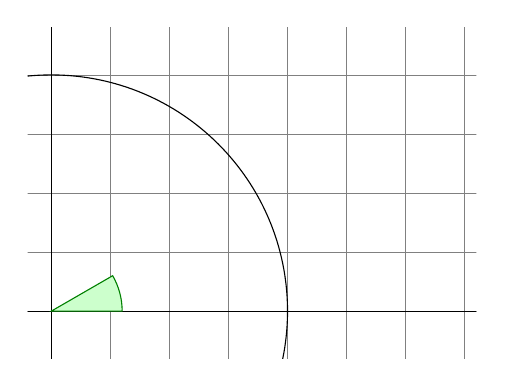
\begin{tikzpicture}[scale=3]
  \clip (-0.1,-0.2)
     rectangle (1.8,1.2);
  \draw[step=.25cm,gray,very thin]
       (-1.4,-1.4) grid (3.4,3.4);
  \draw (-1.5,0) -- (2.5,0);
  \draw (0,-1.5) -- (0,1.5);
  \draw (0,0) circle (1cm);
  \filldraw[fill=green!20!white,
            draw=green!50!black]
    (0,0) -- (3mm,0mm) 
         arc (0:30:3mm) -- cycle;
\end{tikzpicture}
\end{example}
Note the semicolon (\texttt{;}) character. It separates the individual commands.

A simple Venn diagram.
\begin{example}
\shorthandoff{:}
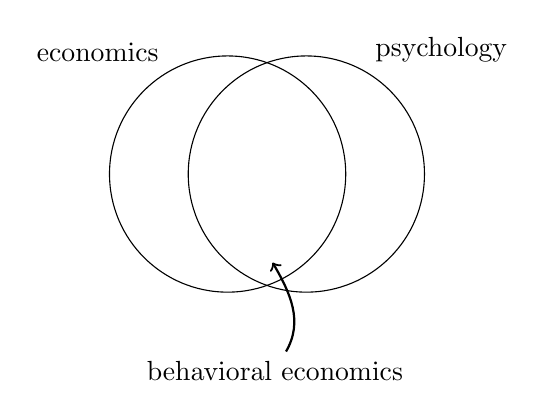
\begin{tikzpicture}
  \node[circle,draw,
        minimum size=3cm,
        label=120:{economics}]
         at (0,0) {};
  \node[circle,draw,
        minimum size=3cm,
        label=60:{psychology}]
         at (1,0) {};
  \node (i) at (0.5,-1) {};
  \node at (0.6,-2.5) 
    {behavioral economics}
    edge[->,thick,
         out=60,in=-60] (i);
\end{tikzpicture}
\end{example}
If you are using \pai{tikz} in connection with \pai{babel} some of the characters used in the
TikZ language may get modified by \pai{babel}, leading to odd errors. To counteract this, add 
the \ci{shorthandoff} command to your code.

Note the foreach loops in the next example.
\begin{example}
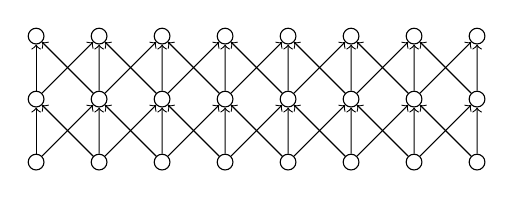
\begin{tikzpicture}[scale=0.8]
  \tikzstyle{v}=[circle, minimum size=2mm,inner sep=0pt,draw]
  \foreach \i in {1,...,8}
    \foreach \j in {1,...,3}
      \node[v] 
        (G-\i-\j) at (\i,\j) {};
  \foreach \i in {1,...,8}
    \foreach \j/\o in {1/2,2/3}
      \draw[->] 
        (G-\i-\j) -- (G-\i-\o);
  \foreach \i/\n in 
    {1/2,2/3,3/4,4/5,5/6,6/7,7/8}
    \foreach \j/\o in {1/2,2/3} {
       \draw[->] (G-\i-\j) -- (G-\n-\o);
       \draw[->] (G-\n-\j) -- (G-\i-\o);
    }
\end{tikzpicture}
\end{example}

With the \ci{usetikzlibrary}
command in the preamble you can enable a wide variety of additional
features for drawing special shapes, like this box which is slightly bent.
\begin{example}
\usetikzlibrary{%
  decorations.pathmorphing}
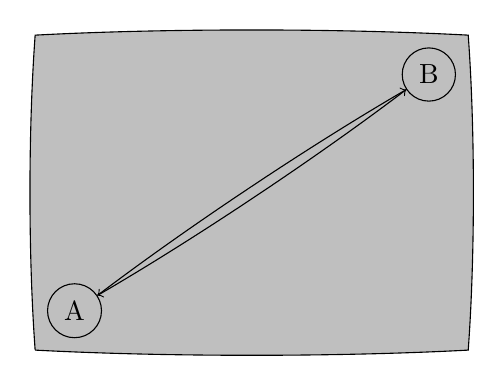
\begin{tikzpicture}[
     decoration={bent,aspect=.3}]
 \draw [decorate,fill=lightgray]
        (0,0) rectangle (5.5,4);
 \node[circle,draw] 
        (A) at (.5,.5) {A};
 \node[circle,draw] 
        (B) at (5,3.5) {B};
 \draw[->,decorate] (A) -- (B);
 \draw[->,decorate] (B) -- (A);
\end{tikzpicture}
\end{example}

\begin{example}
\usetikzlibrary{positioning}
\begin{tikzpicture}[xscale=6,
     yscale=8,>=stealth]
  \tikzstyle{v}=[circle,
     minimum size=1mm,draw,thick]
  \node[v] (a) {$1$};
  \node[v] (b) [right=of a] {$2$};
  \node[v] (c) [below=of a] {$2$};
  \node[v] (d) [below=of b] {$1$};
  \draw[thick,->] 
        (a) to node {} (c);
  \draw[thick,->] 
        (a) to node {} (d);
  \draw[thick,->] 
        (b) to node {} (d);
\end{tikzpicture}
\end{example}

You can even draw syntax diagrams that look as if they came straight from a book on
Pascal programming. The code is a bit more daunting than the example above,
so I will just show you the result. If you have a look at the \pai{pdf} documentation
you will find a detailed tutorial on drawing this exact diagram.

\begin{center}
\begin{tikzpicture}[point/.style={coordinate},thick,draw=black!50,>=stealth',
                    tip/.style={->,shorten >=1pt},every join/.style={rounded corners},
                    skip loop/.style={to path={-- ++(0,#1) -| (\tikztotarget)}},
                    hv path/.style={to path={-| (\tikztotarget)}},
                    vh path/.style={to path={|- (\tikztotarget)}},
                 terminal/.style={
            rounded rectangle,
            minimum size=6mm,
            thick,draw=black!50,
            top color=white,bottom color=black!20,
            font=\ttfamily\tiny},
                nonterminal/.style={
                       rectangle,
                       minimum size=6mm,
                       thick,
                       draw=red!50!black!50,         % 50% red and 50% black,
                       top color=white,              % a shading that is white at the top...
                       bottom color=red!50!black!20, % and something else at the bottom
                       font=\itshape\tiny}]
\matrix[column sep=4mm] {
  % First row:
  & & & & & & & & & & & \node (plus) [terminal] {+};\\
  % Second row:
  \node (p1) [point] {}; &     \node (ui1)    [nonterminal] {unsigned integer}; &
  \node (p2) [point] {}; &     \node (dot)    [terminal]    {.};                &
  \node (p3) [point] {}; &     \node (digit) [terminal]     {digit};            &
  \node (p4) [point] {}; &     \node (p5)     [point] {};                       &
  \node (p6) [point] {}; &     \node (e)      [terminal]    {E};                &
  \node (p7) [point] {}; &                                                      &
  \node (p8) [point] {}; &     \node (ui2)    [nonterminal] {unsigned integer}; &
  \node (p9) [point] {}; &     \node (p10)    [point]       {};\\
  % Third row:
  & & & & & & & & & & & \node (minus)[terminal] {-};\\
};
{ [start chain]
  \chainin (p1);
  \chainin (ui1)   [join=by tip];
  \chainin (p2)    [join];
  \chainin (dot)   [join=by tip];
  \chainin (p3)    [join];
  \chainin (digit) [join=by tip];
  \chainin (p4)    [join];
  { [start branch=digit loop]
    \chainin (p3) [join=by {skip loop=-6mm,tip}];
  }
  \chainin (p5)    [join,join=with p2 by {skip loop=6mm,tip}];
  \chainin (p6)    [join];
  \chainin (e)     [join=by tip];
  \chainin (p7)    [join];
  { [start branch=plus]
    \chainin (plus) [join=by {vh path,tip}];
    \chainin (p8)    [join=by {hv path,tip}];
  }
  { [start branch=minus]
    \chainin (minus) [join=by {vh path,tip}];
    \chainin (p8)    [join=by {hv path,tip}];
  }
  \chainin (p8)    [join];
  \chainin (ui2)   [join=by tip];
  \chainin (p9)    [join,join=with p6 by {skip loop=-11mm,tip}];
  \chainin (p10)   [join=by tip];
}
\end{tikzpicture}
\end{center}

And there is more, if you have to draw plots of numerical data or
functions, you should have a closer look at the  \pai{pgfplot}
package. It provides everything you need to draw plots. It can even
call the external \texttt{gnuplot} command to evaluate actual
functions you wrote into the graph.

For more inspiration make sure to visit Kjell Magne Fauske's excellent \url{http://www.texample.net/tikz/}.
it contains an ever expanding store of beautiful graphs and other \LaTeX{} code.

%%% Local Variables:
%%% TeX-master: "lshort.tex"
%%% mode: flyspell
%%% TeX-PDF-mode: t
%%% End:

%%%%%%%%%%%%%%%%%%%%%%%%%%%%%%%%%%%%%%%%%%%%%%%%%%%%%%%%%%%%%%%%%
% Contents: Customising LaTeX output
% $Id: F-9CC1D91A3ABFA395219F054EDAAEFF48.tex,v 1.1 2008-04-24 16:22:57 carleos Exp $
%%%%%%%%%%%%%%%%%%%%%%%%%%%%%%%%%%%%%%%%%%%%%%%%%%%%%%%%%%%%%%%%%
\chapter{Personalizaci�n de \LaTeX}

\begin{intro}
Los documentos producidos mediante las �rdenes que ha aprendido hasta
este punto parecer�n aceptables a una amplia audiencia.  Aunque no
tienen un aspecto extraordinario, obedecen todas las reglas
establecidas de composici�n correcta, lo que los har� f�ciles de leer
y pl�cidos a la vista.

Sin embargo, hay situaciones donde 
 \LaTeX{} no proporciona una orden o entorno que cubra sus
 necesidades, o la salida producida por algunas �rdenes existentes
 puede no satisfacer sus expectativas.

En este cap�tulo, se dar�n algunas pistas para ense�ar a
\LaTeX{} nuevos trucos y hacerle producir salidas con diferente
aspecto del producido por omisi�n.
\end{intro}


\section{Nuevas �rdenes, entornos y paquetes}

Puede haber notado que todas las �rdenes que presento en este libro se
componen en una caja, y que se muestran en el �ndice al final del
libro.  En lugar de usar directamente las �rdenes \LaTeX{} necesarias
para conseguirlo, he creado un \wi{paquete} en que defino nuevas
�rdenes y entornos con este prop�sito.  Ahora puedo escribir
simplemente:

\begin{example}
\begin{lscommand}
\ci{dum}
\end{lscommand}
\end{example}

En este ejemplo, estoy usando tanto un nuevo entorno llamado\\
\ei{lscommand}, que es responsable de dibujar la caja alrededor de la
orden, y una nueva orden llamada \ci{ci}, que compone el nombre de la
orden y hace la correspondiente entrada en el �ndice.  Puede
comprobarlo buscando la orden \ci{dum} en el �ndice al final del
libro, donde pude encontrar una entrada para \ci{dum}, apuntando a
cada p�gina donde he mencionado la orden \ci{dum}.

Si alguna vez decido que no me gusta que las �rdenes se compongan en
una caja, puedo simplemente cambiar la definici�n del entorno 
\texttt{lscommand} para crear un nuevo aspecto.  Esto es mucho m�s
f�cil que ir por todo el documento localizando todos los lugares en
que he usado comandos \LaTeX{} gen�ricos para dibujar una caja
alrededor de una palabra. 


\subsection{�rdenes nuevas}

Para a�adir sus �rdenes nuevas, use la orden
\begin{lscommand}
\ci{newcommand}\verb|{|%
       \emph{nombre}\verb|}[|\emph{n�m}\verb|]{|\emph{definici�n}\verb|}|
\end{lscommand}
%\noindent command. 
B�sicamente, lo orden requiere dos argumentos: el \emph{nombre} de la
orden que quiere crear, y la \emph{definici�n} de la orden.  El
argumento \emph{n�m} entre corchetes es opcional e indica el n�mero de
argumentos que toma la nueva orden (hasta 9 son posibles).  Si no se
indica el valor es 0, es decir, no se permiten argumentos.

Los siguientes dos ejemplos deber�an ayudarle a entender la idea.  
El primer ejemplo define una nueva orden llamada \ci{intc}.  Es la
abreviatura de ``La introducci�n no-tan-corta a \LaTeXe''.  Tal orden
podr�a ser �til si tuviera que escribir el t�tulo del libro una y otra
vez. 

\begin{example}
\newcommand{\intc}{La 
    introducci�n no-tan-corta a
    \LaTeXe}
Esto es ``\intc'' \ldots{} 
``\intc''
\end{example}

El siguiente ejemplo ilustra c�mo definir una orden nueva que toma un
argumento.
Los caracteres \verb|#1| se sustituyen por el argumento indicado.  Si
quisiera usar un segundo argumento, use \verb|#2| y as� sucesivamente.

\begin{example}
\newcommand{\txsit}[1]
 {Esta es la Introducci�n
   \emph{#1}-corta a \LaTeXe}
% en el cuerpo del documento: 
\begin{itemize}
\item \txsit{no-tan}
\item \txsit{s�per}
\end{itemize}
\end{example}

\LaTeX{} no le permitir� crear una nueva orden sobre una
ya existente.  Pero hay una orden especial en el caso de que
expl�citamente quisiera reemplazarla: \ci{renewcommand}.
Usa la misma sintaxis que la orden \verb|\newcommand|.

En ciertos casos puede querer usar la orden
\ci{providecommand}.  Funciona como \ci{newcommand} y hace que 
la orden sea definida si a�n no existe, pero no hace nada si ya 
estaba definida.

Hay algunos puntos que comentar sobre los espacios que siguen a las
�rdenes de \LaTeX{}.  Vea la p�gina  \pageref{whitespace} para m�s
informaci�n.

\subsection{Nuevos entornos}
Similar a la orden \verb|\newcommand|, hay una orden para crear
sus propios entornos.  La orden \ci{newenvironment} usa la siguiente
sintaxis:

\begin{lscommand}
\ci{newenvironment}\verb|{|%
       \emph{nombre}\verb|}[|\emph{n�m}\verb|]{|%
       \emph{antes}\verb|}{|\emph{despu�s}\verb|}|
\end{lscommand}

Tambi�n \ci{newenvironment} puede tener un argumento opcional.  El
material indicado en el argumento \emph{antes} se procesa antes de que
se procese el texto del entorno.  El material en el argumento
\emph{despu�s} se procesa cuando se encuentra la orden
\verb|\end{|\emph{nombre}\verb|}|.

El ejemplo siguiente ilustra el uso de la orden \ci{newenvironment}.
\begin{example}
\newenvironment{king}
 {\rule{1ex}{1ex}%
      \hspace{\stretch{1}}}
 {\hspace{\stretch{1}}%
      \rule{1ex}{1ex}}

\begin{king} 
Mis humildes ideas...
\end{king}
\end{example}

El argumento \emph{n�m} se usa igual que con la orden
\verb|\newcommand|. \LaTeX{} se asegura de que usted no defina un
entorno que ya existe; pero si quiere alguna vez cambiar un entorno
existente, puede usar la orden \ci{renewenvironment}.  Usa la misma
sintaxis que la orden \ci{newenvironment}.

La orden usada en este ejemplo se explicar� m�s tarde.  Para la orden
\ci{rule} v�ase la p�gina \pageref{sec:rule}, para \ci{stretch} vaya a
la p�gina \pageref{cmd:stretch}, y puede hallar m�s informaci�n sobre
\ci{hspace} en la p�gina \pageref{sec:hspace}.

\subsection{Espacio extra}

Al crear un entorno nuevo puede hallar dificultades en el manejo del
espacio adicional, que puede llegar a tener efectos fatales.  Por
ejemplo, cuando quiera crear un entorno para t�tulos que suprima su
propia sangr�a as� como la del siguiente p�rrafo.  La orden
\ci{ignorespaces} en el bloque de comienzo del entorno har� que �ste
prescinda de cualquier espacio tras ejecutar el bloque de comienzo.
El bloque final requiere un poco m�s de cuidado porque tiene lugar un
proceso especial al final del entorno.  La orden
\ci{ignorespacesafterend} har� que \LaTeX{} ejecute \ci{ignorespaces}
despu�s de que el proceso especial tenga lugar.

\begin{example}
\newenvironment{simple}%
 {\noindent}%
 {\par\noindent}

\begin{simple}
Mire el espacio\\a la izquierda.
\end{simple}
Tambi�n\\aqu�.
\end{example}

\begin{example}
\newenvironment{correct}%
 {\noindent\ignorespaces}%
 {\par\noindent%
   \ignorespacesafterend}

\begin{correct}
Sin espacio\\a la izquierda.
\end{correct}
Tambi�n\\aqu�.
\end{example}

\subsection{L�nea de �rdenes \LaTeX}

Si trabaja en un sistema operativo estilo \textsc{posix} (GNU o \textsc{unix}), quiz�s use \ci{Makefile} para compilar
sus documentos de \LaTeX{}.  Entonces podr�a ser interesante producir
diferentes versiones del mismo documento llamando a \LaTeX{} con diversos 
par�metros en la l�nea de �rdenes.  Si a�ade la siguiente estructura a su
documento:

\begin{verbatim}
\usepackage{ifthen}
\ifthenelse{\equal{\blancoynegro}{verdadero}}{
  % modo "blanco y negro"; hacer algo..
}{
  % modo "color"; hacer algo diferente..
}
\end{verbatim}

Ahora puede llamar a \LaTeX{} as�:
\begin{verbatim}
latex '\newcommand{\blancoynegro}{verdadero}\input{test.tex}'
\end{verbatim}

Primero se define la orden \verb|\blancoynegro| y despu�s se lee el \filenomo{}
real.  Poniendo \verb|\blancoynegro| a falso se producir� la
versi�n en color del documento.

\subsection{Su propio paquete}

Si define muchos nuevos entornos y �rdenes, el pre�mbulo de su
documento se har� muy largo.  En situaciones as� es buena idea crear
un paquete \LaTeX{} que contenga todas sus definiciones de �rdenes y
entornos.  Puede usar despu�s la orden \ci{usepackage} para cargar el
paquete en su documento actual
o en otros similares.

\begin{figure}[!htbp]
\begin{lined}{\textwidth}
\begin{verbatim}
% Paquete Demo de Tobias Oetiker
\ProvidesPackage{demopack}
\newcommand{\intc}{La introducci�n no-tan-corta
                   a \LaTeXe}
\newcommand{\txsit}[1]{La introducci�n \emph{#1}-corta
                       a \LaTeXe}
\newenvironment{king}{\begin{quote}}{\end{quote}}
\end{verbatim}
\end{lined}
\caption{Paquete de ejemplo.} \label{package}
\end{figure}

Escribir un paquete b�sicamente consiste en copiar el contenido del
pre�mbulo de su documento en un \filenomo{} separado con un nombre que
termine en
\texttt{.sty}.  Hay una orden especial,
\begin{lscommand}
\ci{ProvidesPackage}\verb|{|\emph{nombre paquete}\verb|}|
\end{lscommand}
\noindent para usar justo al principio de su \filenomo{} de paquete.
\verb|\ProvidesPackage| dice a  \LaTeX{} el nombre del paquete y le
permite emitir un mensaje de error notable cuando intente incluir el
paquete dos veces.  La figura~\ref{package} muestra un peque�o paquete
de ejemplo que contiene �rdenes definidas en ejemplos anteriores.

\section{\Fontsnomo{} y tama�os}

\subsection{�rdenes que cambian la \fontnomo{}}
\index{\fontnomo{}}\index{tama�o de la \fontnomo{}} \LaTeX{} escoge la
\fontnomo{} y el tama�o de \fontnomo{} apropiados bas�ndose en la
estructura l�gica del documento 
(secciones, notas al pie, ...).   En algunos casos, quiz� desee
cambiar \fontsnomo{} y tama�os a mano.  Para hacerlo, puede usar las
�rdenes listadas en los cuadros~\ref{fonts} y~\ref{sizes}.  El tama�o
real de cada \fontnomo{} es una cuesti�n de dise�o y depende de la clase
de documento y de sus opciones.  El cuadro~\ref{tab:pointsizes}
muestra los tama�os absolutos en puntos para estas �rdenes seg�n se
implementan en las clases de documentos normales.

\begin{example}
{\small Peque�a \textbf{negrita}
 del �frica tropical,}
{\Large grande y \textit{cursi}va
 eres t� ya.}
\end{example}

Una caracter�stica importante de \LaTeXe{} es que los atributos de
\fontnomo{} son independientes.  Esto significa que puede poner �rdenes
para cambiar el tama�o o incluso la \fontnomo{}, y todav�a se mantendr�n
los atributos de negrita o cursiva establecidos anteriormente.

En \emph{modo mates} puede usar las \emph{�rdenes} de cambio de
\fontnomo{} para salir temporalmente del \emph{modo mates} e introducir
texto normal.  Si quiere cambiar a otra \fontnomo{} para composici�n de
mates necesita otro conjunto especial de �rdenes; v�ase el
cuadro~\ref{mathfonts}.

\begin{table}[!bp]
\caption{\Fontsnomo{}.} \label{fonts}
\begin{lined}{12cm}
%
% Alan suggested not to tell about the other form of the command
% eg \verb|\sffamily| or \verb|\bfseries|. This seems a good thing to me.
%
\begin{tabular}{@{}rl@{\qquad}rl@{}}
\fni{textrm}\verb|{...}|        &      \textrm{\wi{rematada}}&
\fni{textsf}\verb|{...}|        &      \textsf{\wi{palo seco}}\\
\fni{texttt}\verb|{...}|        &      \texttt{de m�quina}\\[6pt]
\fni{textmd}\verb|{...}|        &      \textmd{peso medio}&
\fni{textbf}\verb|{...}|        &      \textbf{\wi{negrita}}\\[6pt]
\fni{textup}\verb|{...}|        &       \textup{\wi{recta}}&
\fni{textit}\verb|{...}|        &       \textit{\wi{cursiva}}\\
\fni{textsl}\verb|{...}|        &       \textsl{\wi{oblicua}}&
\fni{textsc}\verb|{...}|        &       \textsc{\wi{Versalitas}}\\[6pt]
\ci{emph}\verb|{...}|          &            \emph{destacada} &
\fni{textnormal}\verb|{...}|    &    \textnormal{por omisi�n}
\end{tabular}

\bigskip
\end{lined}
\end{table}


\begin{table}[!bp]
\index{font size}
\caption{Tama�os de \fontnomo{}.} \label{sizes}
\begin{lined}{12cm}
\begin{tabular}{@{}ll}
\fni{tiny}      & \tiny        \fontnomo{} min�scula \\
\fni{scriptsize}   & \scriptsize  \fontnomo{} muy peque�a\\
\fni{footnotesize} & \footnotesize  bastante peque�a \\
\fni{small}        &  \small          \fontnomo{} peque�a \\
\fni{normalsize}   &  \normalsize  \fontnomo{} normal \\
\fni{large}        &  \large       \fontnomo{} grande
\end{tabular}%
\qquad\begin{tabular}{ll@{}}
\fni{Large}        &  \Large       m�s grande \\[5pt]
\fni{LARGE}        &  \LARGE       muy grande \\[5pt]
\fni{huge}         &  \huge        enorme \\[5pt]
\fni{Huge}         &  \Huge        la m�s
\end{tabular}

\bigskip
\end{lined}
\end{table}

\begin{table}[!tbp]
\caption{Tama�os absolutos en puntos para las clases normales.}\label{tab:pointsizes}
\label{tab:sizes}
\begin{lined}{12cm}
\begin{tabular}{lrrr}
\multicolumn{1}{c}{tama�o} &
\multicolumn{1}{c}{10pt (por omisi�n) } &
           \multicolumn{1}{c}{opci�n 11pt}  &
           \multicolumn{1}{c}{opci�n 12pt}\\
\verb|\tiny|       & 5pt  & 6pt & 6pt\\
\verb|\scriptsize| & 7pt  & 8pt & 8pt\\
\verb|\footnotesize| & 8pt & 9pt & 10pt \\
\verb|\small|        & 9pt & 10pt & 11pt \\
\verb|\normalsize| & 10pt & 11pt & 12pt \\
\verb|\large|      & 12pt & 12pt & 14pt \\
\verb|\Large|      & 14pt & 14pt & 17pt \\
\verb|\LARGE|      & 17pt & 17pt & 20pt\\
\verb|\huge|       & 20pt & 20pt & 25pt\\
\verb|\Huge|       & 25pt & 25pt & 25pt\\
\end{tabular}

\bigskip
\end{lined}
\end{table}


\begin{table}[!bp]
\caption{\Fontsnomo{} para mates.} \label{mathfonts}
\begin{lined}{0.7\textwidth}
\begin{tabular}{@{}ll@{}}
\fni{mathrm}\verb|{...}|&     $\mathrm{Fundici\acute{o}n\ Rematada}$\\
\fni{mathbf}\verb|{...}|&     $\mathbf{Fundici\acute{o}n\ Negrita}$\\
\fni{mathsf}\verb|{...}|&     $\mathsf{Fundici\acute{o}n\ Palo\ Seco}$\\
\fni{mathtt}\verb|{...}|&     $\mathtt{Fundici\acute{o}n\ De\
  M\acute{a}quina}$\\
\fni{mathit}\verb|{...}|&     $\mathit{Fundici\acute{o}n\ Cursiva}$\\
\fni{mathcal}\verb|{...}|&    $\mathcal{FUNDICI\acute{O}N\ CALIGR\acute{A}FICA}$\\
\fni{mathnormal}\verb|{...}|& $\mathnormal{Fundici\acute{o}n\ Normal}$\\
\end{tabular}

%\begin{tabular}{@{}lll@{}}
%\textit{Command}&\textit{Example}&    \textit{Output}\\[6pt]
%\fni{mathcal}\verb|{...}|&    \verb|$\mathcal{B}=c$|&     $\mathcal{B}=c$\\
%\fni{mathscr}\verb|{...}|&    \verb|$\mathscr{B}=c$|&     $\mathscr{B}=c$\\
%\fni{mathrm}\verb|{...}|&     \verb|$\mathrm{K}_2$|&      $\mathrm{K}_2$\\
%\fni{mathbf}\verb|{...}|&     \verb|$\sum x=\mathbf{v}$|& $\sum x=\mathbf{v}$\\
%\fni{mathsf}\verb|{...}|&     \verb|$\mathsf{G\times R}$|&        $\mathsf{G\times R}$\\
%\fni{mathtt}\verb|{...}|&     \verb|$\mathtt{L}(b,c)$|&   $\mathtt{L}(b,c)$\\
%\fni{mathnormal}\verb|{...}|& \verb|$\mathnormal{R_{19}}\neq R_{19}$|&
%$\mathnormal{R_{19}}\neq R_{19}$\\
%\fni{mathit}\verb|{...}|&     \verb|$\mathit{ffi}\neq ffi$|& $\mathit{ffi}\neq ffi$
%\end{tabular}

\bigskip
\end{lined}
\end{table}

En relaci�n a las �rdenes de tama�o de \fontnomo{}, las \wi{llaves}
representan un papel significativo.  Se usan para construir
\emph{grupos}.  Los grupos limitan el alcance de la mayor�a de las
�rdenes de \LaTeX{}.\index{grupos}\index{agrupar}

\begin{example}
Adora los {\LARGE grandes y
{\small peque�os} placeres}. 
\end{example}
 
Las �rdenes de tama�o de \fontnomo{} tambi�n cambian el espaciado entre
renglones, pero s�lo si el p�rrafo termina dentro del �mbito de la
orden de tama�o de \fontnomo{}.  La llave de cierre \verb|}| deber�a por
  tanto no llegar demasiado pronto.  F�jese en la posici�n de la orden
  \ci{par} en los siguientes dos ejemplos.\footnote{\texttt{\bs{}par}
equivale a un rengl�n en blanco.}


\begin{example}
{\Large �No lea esto!
 No es verdad.
 �Puede creerme!\par}
\end{example}

\begin{example}
{\Large Tampoco esto es verdad.
Mas recuerde qu� mendaz soy.}\par
\end{example}

Si quiere activar una orden de cambio de tama�o para un p�rrafo entero
de texto o incluso m�s, puede usar la sintaxis de entorno para las
�rdenes de cambio de \fontnomo{}.

\begin{example}
\begin{Large} 
Esto no es verdad, pero
qu� diantres cabe esperar
en estos tiempos...\par
\end{Large}
\end{example}

\noindent Esto le ahorrar� andar contando llaves.

\subsection{Atenci�n, peligro}

Como se comenta al principio de este cap�tulo, es peligroso sembrar el
documento con �rdenes expl�citas como esas, pues funcionan contra la
idea b�sica de \LaTeX{}, que es separar la estructura de su documento del
aspecto visual.  Esto significa que si usted usa la misma orden de
cambio de \fontnomo{} en varios lugares para componer un tipo especial
de informaci�n, deber�a usar \verb|\newcommand| para definir una
``orden l�gica encubridora'' para la orden de cambio de \fontnomo{}.

\begin{example}
\newcommand{\ojo}[1]{%
 \textbf{#1}}
No \ojo{entre} en esta sala; est� 
ocupada por \ojo{m�quinas} de 
origen y prop�sito desconocidos.
\end{example}

Este enfoque tiene la ventaja de que usted puede decidir en una etapa
posterior que quiere usar alguna representaci�n visual de peligro
distinta de \verb|\textbf|, sin tener que recorrer todo el documento
identificando cada aparici�n de \verb|\textbf| y despu�s deduciendo si
ah� se us� para se�alar un peligro o por alguna otra raz�n.


\subsection{Consejo}

Para concluir este viaje al mundo de las \fontsnomo{} y sus tama�os,
acepte este humilde consejo:\nopagebreak

\begin{quote}
  \underline{\textbf{{\Huge�}Recuerde\Huge!}} \textit{Cuantas}
  \textsf{M\textbf{\LARGE �} \texttt{S}} \textsl{\fontsnomo{}} \Huge use
  \tiny en \footnotesize \textbf{un}  \small \texttt{documento},
  \large \textit{tanto} \normalsize m�s \textsc{legible} y
  \textsl{\textsf{lindo} \large s\Large e\LARGE r\huge �}.
\end{quote}

\section{Espaciado}
 
\subsection{Espacio entre renglones}

\index{espacio entre renglones} Si quiere usar mayor espacio entre
renglones, puede cambiar su valor poniendo la orden
\begin{lscommand}
\ci{linespread}\verb|{|\emph{factor}\verb|}|
\end{lscommand}
\noindent en el pre�mbulo de su documento. 
Use \verb|\linespread{1.3}| para espaciado de ``uno y medio'' y
\verb|\linespread{1.6}| para espaciado ``doble''.  Normalmente los
renglones no se separan, as� que el factor por omisi�n
es~1.\index{doble espaciado de renglones}

Tenga en cuenta que el efecto de la orden \ci{linespread} es bastante
dr�stico y no apropiado para publicar un trabajo.  As� que si tiene una
buena raz�n para cambiar el espacio entre renglones quiz� prefiera
usar la orden:
\begin{lscommand}
\verb|\setlength{\baselineskip}{1.5\baselineskip}|
\end{lscommand}

\begin{example}
{\setlength{\baselineskip}%
           {1.5\baselineskip}
Este p�rrafo est� compuesto con
el salto de l�nea base puesto a
1,5 de lo que era antes.  F�jese
en la orden par al final del
p�rrafo.\par}

Este p�rrafo tiene un prop�sito
claro: mostrar que, una vez se
cierran las llaves, todo vuelve
a la normalidad.
\end{example}

\subsection{Formato de p�rrafo}\label{parsp}

En \LaTeX{}, hay dos par�metros que influyen en el aspecto del
p�rrafo.  Poniendo una definici�n
\begin{code}
\ci{setlength}\verb|{|\ci{parindent}\verb|}{0pt}| \\
\verb|\setlength{|\ci{parskip}\verb|}{1ex plus 0.5ex minus 0.2ex}|
\end{code}
en el pre�mbulo del \filenomo{} de entrada, puede cambiar el aspecto de
los p�rrafos.  Estas dos �rdenes incrementan el espacio entre dos
p�rrafos y establecen la sangr�a de p�rrafo a cero.  

Las partes \texttt{plus} y \texttt{minus} de la longitud de arriba
dicen a 
\TeX{} que puede comprimir y expandir el salto entre p�rrafos la
cantidad indicada, si es necesario para ajustar apropiadamente los
p�rrafos en la p�gina.

En algunos pa�ses europeos los p�rrafos suelen separarse algo y no se
sangran.  Pero tenga en cuenta que esto tiene su efecto en el �ndice
general; sus renglones se espaciar�n m�s en ese caso.  Para evitarlo,
puede mover las dos �rdenes del pre�mbulo a un lugar en su documento
detr�s de la orden \verb|\tableofcontents| o no usarlo en absoluto,
porque ver� que muchos libros profesionales usan sangr�a y no espacio
para separar p�rrafos.

Si quiere sangrar un p�rrafo que no est� sangrado, puede usar
\begin{lscommand}
\ci{indent}
\end{lscommand}
\noindent al principio del p�rrafo. Obviamente,  s�lo tendr� efecto
  cuando \verb|\parindent| no valga cero. Para sangrar el primer
  p�rrafo tras cada t�tulo de secci�n, use el paquete
  \pai{indentfirst} del lote `tools'. 

Para crear un p�rrafo no sangrado, puede usar
\begin{lscommand}
\ci{noindent}
\end{lscommand}
\noindent como primera orden del p�rrafo.  Puede ser �til si empieza
un documento con texto de p�rrafo y no con una orden de secci�n.

\subsection{Espacio horizontal}

\label{sec:hspace}
\LaTeX{} determina los espacios entre palabras y oraciones
autom�ticamente.  Para a�adir espacio horizontal, use:
\index{horizontal!espacio}
\begin{lscommand}
\ci{hspace}\verb|{|\emph{longitud}\verb|}|
\end{lscommand}
Si dicho espacio debiera mantenerse incluso si cae al final o al
principio de rengl�n, use \verb|\hspace*| en lugar de \verb|\hspace|.
La
\emph{longitud} en el caso m�s simple es s�lo un n�mero m�s una
unidad.  Las unidades m�s importantes se listan en el cuadro~\ref{units}. 
\index{unidades}\index{dimensiones}

\begin{example}
�ste\hspace{1.5cm}es un espacio
de 1,5 cm. 
\end{example}
\suppressfloats
\begin{table}[tbp]
\caption{Unidades \TeX{}.} \label{units}\index{unidades}
\begin{lined}{9.5cm} 
\begin{tabular}{@{}ll@{}}
\texttt{mm} & mil�metro $\approx 1/25$~pulgada \quad \demowidth{1mm} \\
\texttt{cm} & cent�metro = 10~mm  \quad \demowidth{1cm}                     \\
\texttt{in} & pulgada $=$ 25,4~mm \quad \demowidth{1in}                    \\
\texttt{pt} & punto $\approx 1/72$~pulgada $\approx \frac{1}{3}$~mm  \quad\demowidth{1pt}\\
\texttt{em} & $\approx$ anchura de una `M' en la \fontnomo{} actual \quad \demowidth{1em}\\
\texttt{ex} & $\approx$ altura de una `x' en la \fontnomo{} actual \quad \demowidth{1ex}
\end{tabular}

\bigskip
\end{lined}
\end{table}

\label{cmd:stretch} 
La orden
\begin{lscommand}
\ci{stretch}\verb|{|\emph{n}\verb|}|
\end{lscommand} 
\noindent genera espacio especial, que se expande hasta llenar todo el
espacio sobrante en un rengl�n.  Si dos �rdenes 
\verb|\hspace{\stretch{|\emph{n}\verb|}}| tienen lugar en el mismo
rengl�n, los espacios crecen proporcionalmente a sus argumentos.

\begin{example}
x\hspace{\stretch{1}}
x\hspace{\stretch{3}}x
\end{example}

Al sar espacio horizontal junto con texto, puede tener sentido hacer
que el espacio ajuste su tama�o en relaci�n con el tama�o de la
\fontnomo{} actual.  Esto puede hacerse usando las unidades relativas a
la \fontnomo{} \texttt{em} y \texttt{ex}:

\begin{example}
{\Large{}gran\hspace{1em}y}\\
{\tiny{}peque�a\hspace{1em}y}
\end{example}
 
\subsection{Espacio vertical}
\LaTeX{} determina
autom�ticamente el espacio entre p�rrafos, secciones, subsecciones, etc. 
Si es necesario, puede a�adirse espacio vertical adicional
\emph{entre dos p�rrafos} con la orden:
\begin{lscommand}
\ci{vspace}\verb|{|\emph{longitud}\verb|}|
\end{lscommand}

Esta orden deber�a usarse normalmente entre dos renglones vac�os.  Si
el espacio debe preservarse en lo alto o en lo bajo de la p�gina, use
la versi�n  de la orden con asterisco, \verb|\vspace*|, en lugar de \verb|\vspace|.
\index{vertical!espacio}

La orden \verb|\stretch|, acompa�ada de \verb|\pagebreak|, puede
usarse para escribir texto en el �ltimo rengl�n de una p�gina, o para
centrar texto verticalmente en una p�gina.
\begin{code}
\begin{verbatim}
Algo de texto...

\vspace{\stretch{1}}
Esto va en la �ltima l�nea de la p�gina. \pagebreak
\end{verbatim}
\end{code}

Espacio adicional entre dos l�neas del 
\emph{mismo} p�rrafo o dentro de una tabla se indica con la orden
\begin{lscommand}
\ci{\bs}\verb|[|\emph{longitud}\verb|]|
\end{lscommand}
\noindent 

Con  \ci{bigskip} y \ci{smallskip} puede saltar una cantidad
predefinida de espacio vertical sin tener que preocuparse de n�meros
exactos.


\section{Composici�n de la p�gina}

\begin{figure}[!hp]
\begin{center}
\makeatletter\@mylayout\makeatother
\end{center}
\vspace*{1.8cm}
\caption{Par�metros de composici�n de la p�gina.}
\label{fig:layout}
\cih{footskip}
\cih{headheight}
\cih{headsep}
\cih{marginparpush}
\cih{marginparsep}
\cih{marginparwidth}
\cih{oddsidemargin}
\cih{paperheight}
\cih{paperwidth}
\cih{textheight}
\cih{textwidth}
\cih{topmargin}
\end{figure}
\index{p�gina!composici�n}
\LaTeXe{} le permite indicar el \wi{tama�o del papel} en la orden \\
\verb|\documentclass|.  Despu�s calcula los \wi{m�rgenes} adecuados,
pero a veces usted no estar� contento con los valores predefinidos.
Naturalmente, puede cambiarlos. 
%no idea why this is needed here ...
\thispagestyle{fancyplain}
La figura~\ref{fig:layout} muestra todos los par�metros que pueden
cambiarse.  La figura se cre� con el paquete \pai{layout} del lote
`tools'.%
\footnote{\CTANref|macros/latex/required/tools|}

\textbf{�ESPERE!} Antes de lanzarse al frenes� de  ``Hagamos esa
p�gina estrecha un poco m�s ancha'', dedique unos segundos a pensar.
Como muchas cosas en \LaTeX, hay una buena raz�n para que el aspecto
de la p�gina sea como es.

Por supuesto, comparada con su p�gina reci�n salida de un paquete
ofim�tico (como OpenOffice Writer o  MS Word), parece horrorosamente
estrecha.  Pero eche un vistazo a su libro favorito\footnote{Me
  refiero a un libro real impreso y producido por una editorial con
  reputaci�n.} y cuente el n�mero de caracteres en una l�nea de texto
normal.  Hallar� que no hay m�s de en torno a 66 caracteres en cada
rengl�n.  Ahora haga lo mismo con su p�gina de \LaTeX{}; ver� lo mismo.  La
experiencia muestra que la lectura se vuelve dif�cil en cuanto hay m�s
caracteres por rengl�n.  Es as� porque a los ojos les resulta dif�cil
moverse desde el final de un rengl�n al principio del siguiente.  Es
la misma raz�n por la que los peri�dicos se componen en m�ltiples
columnas.
As� que si incrementa la anchura de su texto, tenga en cuenta que
est� haciendo la vida m�s dif�cil a los lectores de su documento.  
 
Si de cualquier forma quiere hacerlo, 
\LaTeX{} proporciona dos �rdenes para cambiar estos par�metros.  Se
usan normalmente en el pre�mbulo del documento.

La primera orden asigna un valor fijo a cualquiera de los par�metros:
\begin{lscommand}
\ci{setlength}\verb|{|\emph{par�metro}\verb|}{|\emph{longitud}\verb|}|
\end{lscommand}

La segunda orden a�ade longitud a cualquier par�metro:
\begin{lscommand}
\ci{addtolength}\verb|{|\emph{par�metro}\verb|}{|\emph{longitud}\verb|}|
\end{lscommand} 

Esta segunda orden es de hecho m�s �til que la orden \ci{setlength},
pues puede usted as� trabajar en relaci�n a las valores establecidos.
Para a�adir un cent�metro a la anchura total del texto, pongo las
siguientes �rdenes en el pre�mbulo del documento:
\begin{code}
\verb|\addtolength{\hoffset}{-0.5cm}|\\
\verb|\addtolength{\textwidth}{1cm}|
\end{code}

En este  contexto, quiz� quiera mirar el paquete \pai{calc}.  Le
permite usar operaciones aritm�ticas en el argumento de \ci{setlength}
y en otros lugares donde puede introducir valores num�ricos en
argumentos de funciones.

\section{M�s diversi�n con las longitudes}

Siempre que sea posible, evite usar longitudes absolutas en los
documentos \LaTeX{}.  Intente basar las cosas en la anchura o altura
de otros elementos de la p�gina.  Para la anchura de una figura puede
referirse a \verb|\textwidth| al componer la p�gina.

Las siguientes 3 �rdenes le permiten determinar la anchura, altura y
profundidad de una cadena de texto.

\begin{lscommand}
\ci{settoheight}\verb|{|\emph{variable}\verb|}{|\emph{texto}\verb|}|\\
\ci{settodepth}\verb|{|\emph{variable}\verb|}{|\emph{texto}\verb|}|\\
\ci{settowidth}\verb|{|\emph{variable}\verb|}{|\emph{texto}\verb|}|
\end{lscommand}

\noindent El ejemplo siguiente muestra una posible aplicaci�n de estas
�rdenes.

\begin{example}
\flushleft
\newenvironment{vardesc}[1]{%
  \settowidth{\parindent}{#1:\ }
  \makebox[0pt][r]{#1:\ }}{}

\begin{displaymath}
a^2+b^2=c^2
\end{displaymath}

\begin{vardesc}{Donde}$a$, 
$b$ -- son adyacentes al �ngulo
recto de un tri�ngulo rect�ngulo.

$c$ -- es la hipotenusa del
tri�ngulo, y 

$d$ -- no sale aqu�
en absoluto. 
\end{vardesc}
\end{example}

\section{Cajas}
\LaTeX{} construye sus p�ginas colocando cajas.  En principio, cada
letra es una cajita, que se pega a otras letras para formar palabras.
�stas se pegan de nuevo a otras palabras, pero con un pegamento
especial, que es tan el�stico que una serie de palabras puede
comprimirse o expandirse para rellenar exactamente un rengl�n de la
p�gina. 

Esto es una simplificaci�n de lo que realmente
ocurre, pero realmente ocurre: \TeX{} trabaja con pegamento y cajas.
Las letras no son las �nicas cosas que son cajas.  Puede poner
virtualmente cualquier cosa en una caja, incluso otras cajas.  Cada
caja ser� manejada por \LaTeX{} como si fuera una simple letra.

En los cap�tulos anteriores ya ha encontrado algunas cajas, aunque no
lo parezcan.  Los entornos \ei{tabular} e
\ci{includegraphics}, por ejemplo, producen cajas.  Esto significa que
puede usted f�cilmente colocar dos tablas o im�genes una al lado de la
otra.  Basta con asegurarse de que su anchura combinada no excede la
anchura del texto.

Puede tambi�n empaquetar un p�rrafo de su elecci�n en una caja con la
orden

\begin{lscommand}
\ci{parbox}\verb|[|\emph{pos}\verb|]{|\emph{anchura}\verb|}{|\emph{texto}\verb|}|
\end{lscommand}

\noindent o el entorno

\begin{lscommand}
\verb|\begin{|\ei{minipage}\verb|}[|\emph{pos}\verb|]{|\emph{anchura}\verb|}| texto 
\verb|\end{|\ei{minipage}\verb|}|
\end{lscommand}

\noindent El par�metro \texttt{pos} puede tomar una de las letras 
\texttt{c, t} o \texttt{b} para controlar la alineaci�n vertical de la
caja, relativa a la l�nea base del texto que la
rodea. \texttt{anchura} toma como argumento la longitud que indica la
anchura de la caja.  La principal diferencia entre una \ei{minipage} y
una \ci{parbox} es que usted no puede usar todas las �rdenes y
entornos dentro de una \ei{parbox}, mientras que casi todo es posible
en una \ei{minipage}.

Mientras que \ci{parbox} empaqueta un p�rrafo entero partiendo
renglones y todo, hay tambi�n una clase de �rdenes encajonadoras que
trabajan s�lo con material alineado horizontalmente.  Ya conocemos una
de ellas; se llama \ci{mbox}.  Simplemente empaqueta una serie de
cajas en otra, y puede usarse para impedir a \LaTeX{} romper dos
palabras.  Como puede  poner cajas dentro de cajas, estos
empaquetadores de cajas horizontales le dan total flexibilidad.

La orden
\begin{lscommand}
\ci{makebox}\verb|[|\emph{anchura}\verb|][|\emph{pos}\verb|]{|\emph{texto}\verb|}|
\end{lscommand}

\noindent donde \texttt{anchura} define la anchura de la caja resultante
vista desde fuera,\footnote{Esto significa que puede ser m�s peque�a
  que el material dentro de ella.  Usted puede incluso poner la
  anchura 0pt de forma que el texto de dentro de la caja se componga
  sin afectar a las cajas de alrededor.}  tiene un efecto parecido.
Adem�s de las expresiones de
longitud, puede tambi�n usar \ci{width}, \ci{height}, \ci{depth} y
\ci{totalheight} en el par�metro de anchura.  Se establecen a partir
de valores obtenidos midiendo el \emph{texto} compuesto.  El par�metro
\emph{pos} toma una letra como valor: \textbf{c}enter (centro),
flush\textbf{l}eft (izquierda),
flush\textbf{r}ight (derecha) o \textbf{s}pread (expandir el texto
hasta llenar la caja).

La orden \ci{framebox} funciona exactamente igual que \ci{makebox},
pero dibuja una caja alrededor del texto.

El ejemplo siguiente le muestra algunas cosas que podr�a hacer con las
�rdenes \ci{makebox} y \ci{framebox}.

\begin{example}
\makebox[\textwidth]{%
    c e n t r a d o}\par
\makebox[\textwidth][s]{%
    e x p a n d i d o}\par
\framebox[1.1\width]{A la medida} \par
\framebox[0.8\width][r]{Muy ancho} \par
\framebox[1cm][l]{Y otro tambi�n...} 
�Puede leer esto?
\end{example}

Ahora que controlamos lo horizontal, el siguiente paso obvio es ir por
la vertical.\footnote{El control total s�lo se obtiene controlando 
tanto lo horizontal como lo vertical...}

La orden
\begin{lscommand}
\ci{raisebox}\verb|{|\emph{sube}\verb|}[|\emph{extiende-sobre-l�nea-base}\verb|][|\emph{extiende-bajo-l�nea-base}\verb|]{|\emph{texto}\verb|}|
\end{lscommand}
\noindent le permite definir las propiedades verticales de una caja.
Puede usar \ci{width}, \ci{height}, \ci{depth} y
  \ci{totalheight} en los tres primeros par�mtros, para afectar al
  tama�o de la caja dentro del argumento \emph{texto}.


\begin{example}
\raisebox{0pt}[0pt][0pt]{\Large%
\textbf{Aaaa\raisebox{-0.3ex}{a}%
\raisebox{-0.7ex}{aa}%
\raisebox{-1.2ex}{h}%
\raisebox{-2.2ex}{h}%
\raisebox{-4.5ex}{h}}}
---grit�, pero ni siquiera el m�s
pr�ximo se dio cuenta de que 
algo terrible le hab�a sucedido...
\end{example}

\section{L�neas y puntales}
\label{sec:rule}

Hace unas p�ginas puede haber visto la orden

\begin{lscommand}
\ci{rule}\verb|[|\emph{sube}\verb|]{|\emph{anchura}\verb|}{|\emph{altura}\verb|}|
\end{lscommand}

\noindent Usada normalmente produce simplemente una caja negra.

\begin{example}
\rule{3mm}{.1pt}%
\rule[-1mm]{5mm}{1cm}%
\rule{3mm}{.1pt}%
\rule[1mm]{1cm}{5mm}%
\rule{3mm}{.1pt}
\end{example}

\noindent Esto es �til para dibujar l�neas verticales y horizontales.
La l�nea de la p�gina del t�tulo, por ejemplo, ha sido creada con una
orden \ci{rule}.

Un caso especial es una l�nea sin anchura pero con cierta altura.  En
composici�n profesional se llama \wi{puntal}.  Se usa para garantizar
que un elemento de una p�gina tiene una cierta altura m�nima.  Podr�a
usarlo en un entorno \texttt{tabular} para asegurarse de que una fila
tiene cierta altura m�nima.

\begin{example}
\begin{tabular}{|c|}
\hline
\rule{1pt}{4ex}Costeru...\\
\hline
\rule{0pt}{4ex}Puntal\\
\hline
\end{tabular}
\end{example}

\bigskip
{\flushright Fin.\par}

%

% Local Variables:
% TeX-master: "lshort2e"
% mode: latex
% mode: flyspell
% End:

\appendix
\chapter{Installing \LaTeX}
\begin{intro}
Knuth published the source to \TeX{} back in a time when nobody knew
about OpenSource and/or Free Software. The License that comes with \TeX{}
lets you do whatever you want with the source, but you can only call the
result of your work \TeX{} if the program passes a set of tests Knuth has
also provided. This has lead to a situation where we have free \TeX{}
implementations for almost every Operating System under the Sun. In this chapter
you will give some hints on what to install on Linux, Mac OS X and Windows to
get \TeX{} working.
\end{intro}

\section{What to Install}

For using LaTeX on any computer system, you need several programs.

\begin{enumerate}

\item The \TeX{}/\LaTeX{} program for processing your \LaTeX{} source files
into typeset PDF or DVI documents.

\item A text editor for editing your LaTeX source files. Some products even let
you start the latex program from within the editor.

\item A PDF/DVI viewer program for previewing and printing your
documents.

\item A program to handle \PSi{} files and images for inclusion into
your documents.

\end{enumerate}

For all platforms there are many programs that fit the requirements above.
Here we just tell about the ones we know, like and have some experience
with.

\section{\TeX{} on Mac OS X}

\subsection{Get a \TeX{} Distribution}

Just download \wi{MacTeX}. It is a
pre-compiled LaTeX distribution for OS X. \wi{MacTeX} provides a full LaTeX
installation plus a number of additional tools. Get MaxTeX from
\url{http://www.tug.org/mactex/}.

If you are already using Macports or Fink for installing Unix software under
OS X, install LaTeX using these package managers. Macport users install
LaTeX with \framebox{\texttt{port install texlive}},
Fink users use the command \framebox{\texttt{fink install texlive}}.

\subsection{Picking an Editor}

The most popular open source editor for \LaTeX{} on the mac seems to be
\TeX{}shop.  Get a copy from \url{http://www.uoregon.edu/~koch/texshop}. It
is also contained in the \wi{MacTeX} distribution.

Another fine editor is Texmaker. Apart from being a useful editor it has the
advantage of running on Windows, Mac and Unix/Linux equally well. Go to
\url{http://www.xm1math.net/texmaker} for further Information. Note there is
also a forked version of Texmaker called TexmakerX on
\url{http://texmakerx.sourceforge.net/} it promises additional functionality.

Recent \TeX Live distributions contain the \TeX{}works editor 
\url{http://texworks.org/} which is a multi-platform editor based on the \TeX{}Shop
design. Since \TeX{}works uses the Qt toolkit, it is available on any platform
supported by this toolkit (MacOS X, Windows, Linux.) 

\subsection{Treat yourself to \wi{PDFView}}

Use PDFView for viewing PDF files generated by LaTeX, it integrates tightly
with your LaTeX text editor. PDFView is an open-source application can be
downloaded from the PDFView website on\\
\url{http://pdfview.sourceforge.net/}. Download and install PDFView. Open
PDFViews preferences dialog and make sure that the \emph{automatically reload
documents} option is enabled and that PDFSync support is set to the TextMate
preset.

\section{\TeX{} on Windows}

\subsection{Getting \TeX{}}

First, get a copy of the excellent MiK\TeX\index{MiKTeX@MiK\TeX} distribution from\\
\url{http://www.miktex.org/}. It contains all the basic programs and files
required to compile \LaTeX{} documents.  The coolest feature in my eyes, is
that MiKTeX will download missing \LaTeX{} packages on the fly and install them
magically while compiling a document. Alternatively you can also use
the TeXlive distribution which exists for Windows, Unix and Mac OS to
get your base setup going \url{http://www.tug.org/texlive/}.

\subsection{A \LaTeX{} editor}

\LaTeX{} is a programming language for text documents. \wi{TeXnicCenter}
uses many concepts from the programming-world to provide a nice and
efficient \LaTeX{} writing environment in Windows. Get your copy from\\
\url{http://http://www.texniccenter.org/}. TeXnicCenter integrates nicely with
MiKTeX. Version 2.0 of TeXnicCenter will support Unicode, the recent alpha version
seems to be quite stable.

Other excellent choice is the editor provided by the LEd project available
on \url{http://www.latexeditor.org}.

See the note on Texmaker in the Mac section above for a third choice.

Recent \TeX Live distributions contain the \TeX{}works Editor
\url{http://texworks.org/}. It supports Unicode and requires at least Windows XP.

\subsection{Document Preview}

You will most likely be using Yap for DVI preview as it gets installed with
MikTeX. For PDF you may want to look at Sumatra
PDF \url{http://blog.kowalczyk.info/software/sumatrapdf/}. I mention Sumatra PDF
because it lets you jump from any position in the pdf document back into
corresponding position in your source document.

\subsection{Working with graphics}

Working with high quality graphics in \LaTeX{} means that you have to use
\EPSi{} (eps) or PDF as your picture format. The program that helps you
deal with this is called \wi{GhostScript}. You can get it, together with its
own front-end \wi{GhostView}, from \url{http://www.cs.wisc.edu/~ghost/}.

If you deal with bitmap graphics (photos and scanned material), you may want
to have a look at the open source photoshop alternative \wi{Gimp} available
from \url{http://gimp-win.sourceforge.net/}.

\section{\TeX{} on Linux}

If you work with Linux, chances are high that \LaTeX{} is already installed
on your system, or at least available on the installation source you used to
setup. Use your package manager to install the following packages:

\begin{itemize}
\item texlive -- the base \TeX{}/\LaTeX{} setup.
\item emacs (with auctex) -- a Linux editor that integrates tightly with \LaTeX{} through the add-on AucTeX package.
\item ghostscript -- a \PSi{} preview program.
\item xpdf and acrobat -- a PDF preview program.
\item imagemagick -- a free program for converting bitmap images.
\item gimp -- a free photoshop look-a-like.
\item inkscape -- a free illustrator/corel draw look-a-like.
\end{itemize}

If you are looking for a more windows like graphical editing environment,
check out Texmaker or \TeX{}works. See the note in the Mac section above.

Most Linux distros insist on splitting up their \TeX{} environments into a
large number of optional packages, so if something is missing after your
first install, go check again.

\backmatter
%%%%%%%%%%%%%%%%%%%%%%%%%%%%%%%%%%%%%%%%%%%%%%%%%%%%%%%%%%%%%%%%%
% Contents: The Bibliography
% File: biblio.tex (lshort2e.tex)
% $Id: biblio.tex 449 2010-12-14 16:53:51Z oetiker $
%%%%%%%%%%%%%%%%%%%%%%%%%%%%%%%%%%%%%%%%%%%%%%%%%%%%%%%%%%%%%%%%%
\begin{thebibliography}{99}
\addcontentsline{toc}{chapter}{\bibname} 
\bibitem{manual} Leslie Lamport.  \newblock \emph{{\LaTeX:} A Document
    Preparation System}.  \newblock Addison-Wesley, Reading,
  Massachusetts, second edition, 1994, ISBN~0-201-52983-1.
  
\bibitem{texbook} Donald~E. Knuth.  \newblock \textit{The \TeX{}book,}
  Volume~A of \textit{Computers and Typesetting}, Addison-Wesley,
  Reading, Massachusetts, second edition, 1984, ISBN~0-201-13448-9.

\bibitem{companion} Frank Mittelbach, Michel Goossens, Johannes Braams,
  David Carlisle, Chris Rowley.  \newblock \emph{The {\LaTeX} Companion, (2nd Edition)}.  \newblock
  Addison-Wesley, Reading, Massachusetts, 2004, ISBN~0-201-36299-6.

\bibitem{graphicscompanion} Michel Goossens, Sebastian Rahtz and Frank
  Mittelbach.  \newblock \emph{The {\LaTeX} Graphics Companion}.  \newblock
  Addison-Wesley, Reading, Massachusetts, 1997, ISBN~0-201-85469-4.
 
\bibitem{local} Each \LaTeX{} installation should provide a so-called
  \emph{\LaTeX{} Local Guide}, which explains the things that are
  special to the local system.  It should be contained in a file called
  \texttt{local.tex}. Unfortunately, some lazy sysops do not provide such a
  document. In this case, go and ask your local \LaTeX{} guru for help.
 
\bibitem{usrguide} \LaTeX3 Project Team.  \newblock \emph{\LaTeXe~for
    authors}.  \newblock Comes with the \LaTeXe{} distribution as
  \texttt{usrguide.tex}.

\bibitem{clsguide} \LaTeX3 Project Team.  \newblock \emph{\LaTeXe~for
    Class and Package writers}.  \newblock Comes with the \LaTeXe{}
  distribution as \texttt{clsguide.tex}.

\bibitem{fntguide} \LaTeX3 Project Team.  \newblock \emph{\LaTeXe~Font
    selection}.  \newblock Comes with the \LaTeXe{} distribution as
  \texttt{fntguide.tex}.

\bibitem{graphics} D.~P.~Carlisle.  \newblock \emph{Packages in the
    `graphics' bundle}.  \newblock Comes with the `graphics' bundle as
  \texttt{grfguide.tex}, available from the same source your \LaTeX{}
  distribution came from.

\bibitem{verbatim} Rainer~Sch\"opf, Bernd~Raichle, Chris~Rowley.  
\newblock \emph{A New Implementation of \LaTeX's verbatim
  Environments}.
 \newblock Comes with the `tools' bundle as
  \texttt{verbatim.dtx}, available from the same source your \LaTeX{}
  distribution came from. 

\bibitem{cyrguide} Vladimir Volovich, Werner Lemberg and \LaTeX3 Project Team.                    
    \newblock \emph{Cyrillic languages support in \LaTeX}.                                        
    \newblock Comes with the \LaTeXe{} distribution as                                            
  \texttt{cyrguide.tex}.                                                                          

\bibitem{catalogue} Graham~Williams.  \newblock \emph{The TeX
    Catalogue} is a very complete listing of many \TeX{} and \LaTeX{}
    related packages.
  \newblock Available online from \CTAN|help/Catalogue/catalogue.html|
  
\bibitem{eps} Keith~Reckdahl.  \newblock \emph{Using EPS Graphics in
    \LaTeXe{} Documents}, which explains everything and much more than
  you ever wanted to know about EPS files and their use in \LaTeX{}
  documents.  \newblock Available online from
  \CTAN|info/epslatex.ps|

\bibitem{xy-pic} Kristoffer H. Rose.
  \newblock \emph{\Xy-pic User's Guide}.  \newblock
  Downloadable from CTAN with \Xy-pic distribution 
  
\bibitem{metapost} John D. Hobby.
  \newblock \emph{A User's Manual for \MP}. \newblock
  Downloadable from \url{http://cm.bell-labs.com/who/hobby/} 
  
\bibitem{unbound} Alan Hoenig.
  \newblock \emph{\TeX{} Unbound}. \newblock Oxford University Press, 1998,
    ISBN 0-19-509685-1; 0-19-509686-X (pbk.) 
  
\bibitem{ursoswald} Urs Oswald.  
    \newblock \emph{Graphics in \LaTeXe{}}, containing some Java source files for 
    generating arbitrary circles and ellipses within the \texttt{picture} environment,
    and \emph{\MP{} - A Tutorial}.
  \newblock Both downloadable from \url{http://www.ursoswald.ch}

\bibitem{pgfplot} Till Tantau.
  \newblock \emph{TikZ\&PGF Manual}.\newblock
  Download from \CTAN|graphics/pgf/base/doc/generic/pgf/pgfmanual.pdf|

% new items for XeLaTeX
\bibitem{polyglossia} Fran\c{c}ois Charette.                    
    \newblock \emph{Polyglossia: A Babel Replacement for \hologo{XeLaTeX}}.                                        
    \newblock Comes with the \TeX Live distribution as                                            
  \texttt{polyglossia.pdf}. (Type \texttt{texdoc polyglossia} on the command line.)

\bibitem{arabxetex} Fran\c{c}ois Charette.                    
    \newblock \emph{An Arab\TeX-like interface for typesetting languages
     in Arabic script with \hologo{XeLaTeX}}.                                        
    \newblock Comes with the \TeX Live distribution as                                            
  \texttt{arabxetex.pdf}. (Type \texttt{texdoc arabxetex} on the command line.)

\bibitem{fontspec} Will Robertson and Khaled Hosny.                    
    \newblock \emph{The \texttt{fontspec} package}.                                        
    \newblock Comes with the \TeX Live distribution as                                            
  \texttt{fontspec.pdf}. (Type \texttt{texdoc fontspec} on the command line.)
    
\bibitem{xgreek} Apostolos Syropoulos.                    
    \newblock \emph{The \texttt{xgreek} package}.                                        
    \newblock Comes with the \TeX Live distribution as                                            
  \texttt{xgreek.pdf}. (Type \texttt{texdoc xgreek} on the command line.)

\bibitem{bidi} Vafa Khalighi.                    
    \newblock \emph{The \texttt{bidi} package}.                                        
    \newblock Comes with the \TeX Live distribution as                                            
  \texttt{bidi.pdf}. (Type \texttt{texdoc bidi} on the command line.

\bibitem{xepersian} Vafa Khalighi.                    
    \newblock \emph{The \texttt{XePersian} package}.                                        
    \newblock Comes with the \TeX Live distribution as                                            
  \texttt{xepersian-doc.pdf}. (Type \texttt{texdoc xepersian} on the command line.

\bibitem{xecjk} Wenchang Sun.                    
    \newblock \emph{The \texttt{xeCJK} package}.                                        
    \newblock Comes with the \TeX Live distribution as                                            
  \texttt{xeCJK.pdf}. (Type \texttt{texdoc xecjk} on the command line.

\end{thebibliography}


%

% Local Variables:
% TeX-master: "lshort2e"
% mode: latex
% mode: flyspell
% End:

\refstepcounter{chapter}
\addcontentsline{toc}{chapter}{Index} 
\printindex
\end{document}





%

% Local Variables:
% TeX-master: "lshort2e"
% mode: latex
% mode: flyspell
% End:
